\documentclass{article}

% Packages
\usepackage{enumitem}   
\usepackage{amsmath}
\usepackage{amsfonts}
\usepackage{mathtools}
\usepackage{tikz}
\usepackage{tikz-3dplot}
\usepackage{tabto}
\usepackage{centernot}
\usepackage{amssymb}
\usepackage{amsthm}
\usepackage{graphicx} % For including images
\usepackage{float} 
\usepackage[backend=biber, style=numeric]{biblatex}
\usepackage{biblatex} % For bibliography management
\usepackage[pdfencoding=auto, psdextra]{hyperref}
\hypersetup{
    colorlinks,
    linktoc=all,
    linkcolor={blue},
    citecolor={blue},
    urlcolor={blue}
}
\addbibresource{references.bib}
\usetikzlibrary{decorations.pathreplacing}

% Redefined Commands
\DeclareRobustCommand{\rchi}{{\mathpalette\irchi\relax}}
\newcommand*\diff{\mathop{}\!\mathrm{d}}
\newcommand\myfunc[5]{%
  \begingroup
  \setlength\arraycolsep{0pt}
  #1\colon\begin{array}[t]{c >{{}}c<{{}} c}
             #2 & \to & #3 \\ #4 & \mapsto & #5 
          \end{array}%
  \endgroup}
\DeclareMathOperator*{\esssup}{ess\,sup}
\newcommand{\myquad}[1][1]{\hspace*{#1em}\ignorespaces}
\newcommand*\circled[1]{\tikz[baseline=(char.base)]{
            \node[shape=circle,draw,inner sep=2pt] (char) {#1};}}
\newcommand{\irchi}[2]{\raisebox{\depth}{$#1\chi$}} % inner command, used by \rchi
\newcommand{\chapquote}[3]{\begin{quotation} \textit{#1} \end{quotation} \begin{flushright} - #2\end{flushright} }
\newcommand{\cnorm}[0]{\Vert \cdot \Vert}
\newcommand{\hookuparrow}{\mathrel{\rotatebox[origin=c]{90}{$\hookrightarrow$}}}
\newcommand{\hookdownarrow}{\mathrel{\rotatebox[origin=c]{-90}{$\hookrightarrow$}}}
\newcommand{\spann}[0]{\mathrm{span}}
\newcommand{\weakstar}[0]{\stackrel{\ast}{\rightharpoonup}}
\newcommand{\scalar}[2]{\langle  {#1} , {#2} \rangle}



% Front page, title
\title{Real and Functional Analysis%

  \large Notes from a course by prof. Gianmaria Verzini\\
    Politecnico di Milano, A.Y. 2024/2025}
\author{Alessandro Cavalieri}
\date{October 2024}

\begin{document}
\maketitle
%Table of Contents
\tableofcontents

% Chapters
\section{Set Theory}
\chapquote{``A set is a Many that allows itself to be thought of as a One."}{Georg Cantor}

In questa sezione vengono presentate principalmente definizioni che forniranno la base per la trattazione dei successivi capitoli.
\subsection{Teoria di Zermelo-Frankel}
\subsection{Famiglie di insiemi}
\subsubsection{(axiom) Power set}
Sia $X$ un insieme. Denotiamo con $\mathcal P(X)$ l'insieme delle parti di $X$, definito come segue:
$$\mathcal P(X)\coloneqq \{ Y : Y\subseteq X\}$$
L'esistenza del power set è uno degli assiomi della Teoria degli Insiemi di Zermelo-Fraenkel.
\begin{figure}[H] % [H] makes sure the figure is placed exactly here
    \centering
    \includegraphics[width=0.7\textwidth]{assets/sets-5b180229ff1b780036cfb499.jpg}
    \caption{Insieme delle parti}
    \label{fig:example_image}
\end{figure}
Denotiamo con $\{E_i\}_{i\in I}$ una famiglia di insiemi indicizzata da I.\\

Una famiglia (o collezione) di sottoinsiemi di un insieme $X$ è $\{E_i\}_{i\in I}\subseteq \mathcal P(X)$
\subsubsection{(def) Union of a family of subsets}
Given a family $\{E_i\}_{i\in I}\subseteq \mathcal P(X)$,
$$\bigcup_{i\in I} E_i = \{x\in X\ : \ x\in E_i \text{ for some } i\in I\}$$
\subsubsection{(def) Intersection of a family of subsets}
Given a family $\{E_i\}_{i\in I}\subseteq \mathcal P(X)$,
$$\bigcap_{i\in I} E_i = \{x\in X\ : \ x\in E_i \text{ for every } i\in I\}$$
\subsubsection{(def) Pairwise disjoint family}
Una famiglia di insiemi $\{E_i\}_{i\in I}$ è detta disgiunta se
$$E_i\cap E_j=\emptyset \quad \forall i,j\in I:i\neq j$$
\subsubsection{(def) Convering set}
Una famiglia di insiemi $\{E_i\}_{i\in I}$ è detta copertura di $X$ se $$X\subseteq \bigcup_{i\in I}E_i$$
\subsubsection{(def) Subcovering}
Si definisce sottocopertura una sottofamiglia di una copertura di $X$ tale per cui essa stessa è ancora una copertura di $X$.
$$X\subseteq \bigcup_{i\in J}E_i\quad J\subset I$$
\subsection{Successioni di insiemi}
Le successioni (o sequenze) di insiemi sono un caso particolare di famiglia di insiemi in cui $I=\mathbb N$. Si denotano con $\{E_n\}_{n\in \mathbb N}$.
\subsubsection{(def) subsequence}
Una sottosequenza è una sequenza derivata da un'altra sequenza selezionando alcuni dei suoi elementi, mantenendo il loro ordine relativo.

Sia $\{E_n\}_{n\in \mathbb N}$ una sequenza. Una sottosequenza di $\{E_n\}_{n\in \mathbb N}$ è una sequenza della forma $\{E_{n_k}\}_{k\in \mathbb N}$
\subsubsection{(def) Monotone increasing (decreasing) sequence}
Una sequenza $ \{E_n\}_n\subseteq \mathcal P(X)$ è detta monotona crescente se:
$$E_{n}\subseteq E_{n+1} \quad \forall n \in \mathbb N$$

Analogamente, una sequenza $ \{E_n\}_n\subseteq \mathcal P(X)$ è detta monotona decrescente se:
$$E_{n}\supseteq E_{n+1} \quad \forall n \in \mathbb N$$


\subsubsection{(def) limsup e liminf di successioni di insiemi}
Considerando una sequenza $\{E_n\}_n\subseteq \mathcal P(X)$. Definiamo:
$$\limsup_n E_n = \bigcap_{k=1}^{+\infty}\Big [\bigcup_{n=k}^{+\infty} E_n\Big ]$$
$$\liminf_n E_n = \bigcup_{k=1}^{+\infty}\Big [\bigcap_{n=k}^{+\infty} E_n\Big ]$$
$$\limsup_n E_n=\liminf_n E_n=F \implies \lim_nE_n=F$$
\subsubsection{(def) Funzione caratteristica di un insieme}
Sia $E\subseteq X$, si definisce funzione caratteristica (o funzione indicatrice) la funzione $$\rchi_E(x)=\begin{cases}1\quad \text{se }x\in E\\0\quad\text{altrimenti}\end{cases}$$

\subsection{Relazioni}
Sia $X$ un insieme. Una relazione su $X$ è un sottoinsieme del prodotto cartesiano $R\subseteq X\times X$.
\subsubsection{(def) Relazione di equivalenza}
Una relazione $R$ si dice relazione di equivalenza e si indica con $\sim$ se soddisfa le seguenti proprietà:
\begin{enumerate}[label=\roman*]
    \item Riflessività $$(x,x)\in R\quad \forall x\in X$$
    \item Simmetria $$(x,y)\in R \iff (y,x)\in R$$
    \item Transitività $$\begin{cases}(x,y)\in R\\(y,z)\in R\end{cases}\implies (x,z)\in R$$
\end{enumerate}
Notazioni equivalenti: $(x,y)\in R \leftrightarrow xRy \leftrightarrow x\sim y$
\subsubsection{(def) classe di equivalenza}
Dato $a\in X$ e $\sim $ una relazione di equivalenza, definiamo:
$$[a]\coloneqq \{x\in X: x\sim a\}$$
la classe di equivalenza di $a$ su $X$.
\subsubsection{(prop) proprietà della classe di equivalenza}
\begin{enumerate}
    \item Ogni elemento di $X$ appartiene a una e una sola classe di equivalenza.
    \item Le classi di equivalenza formano una partizione di $X$, cioè suddividono $X$ in sottoinsiemi disgiunti, tali che la loro unione dà l'intero insieme $X$.
    $$X=\bigcup_{x\in X}[x]$$
\end{enumerate}
\subsubsection{(def) quotient set}
Il quotient set (insieme quoziente) è il risultato della "divisione" di un insieme $X$ in classi di equivalenza rispetto a una data relazione di equivalenza $\sim$.

L'insieme quoziente contiene quindi tutte le classi di equivalenza dell'insieme $X$ ed è una partizione di $X$.
$$\frac X R\coloneqq\{ [x]:x\in X\}$$
\subsubsection{(def) relazione d'ordine}
Una relazione d'ordine è una relazione binaria che stabilisce un confronto tra gli elementi di un insieme $X$, definendo un criterio di ordinamento.

Vi sono diversi tipi di relazioni d'ordine:
\begin{itemize}
    \item \textbf{Relazione di quasi ordine} se soddisfa le seguenti proprietà:
        \begin{enumerate}[label=\roman*]
            \item Riflessività $$xRx\quad \forall x\in X$$
            \item Transitività $$xRy , \ yRz\implies xRz$$
        \end{enumerate}
    \item \textbf{Relazione d'ordine parziale} se soddisfa le seguenti proprietà:
        \begin{enumerate}[label=\roman*]
            \item Riflessività $$xRx\quad \forall x\in X$$
            \item Antisimmetria $$xRy, yRx \implies x=y$$
            \item Transitività $$xRy , \ yRz\implies xRz$$
        \end{enumerate}
        Questo tipo di relazione permette di confrontare alcuni, ma non necessariamente tutti, gli elementi di $X$. Ci possono essere elementi non comparabili tra loro.
    \item \textbf{Relazione d'ordine totale (o lineare, o "catena")} se soddisfa le proprietà di un ordine parziale e si ha la connessione, ovvero $\forall a,b\in X$, vale o $aRb$ o $bRa$. Ovvero, ogni coppia di elementi è comparabile.
\end{itemize}
Ad esempio:
\begin{itemize}
    \item Ordine sui numeri reali: si sostituisca R con "$\le$". è un esempio di ordine totale.
    \item Sottoinsiemi di un insieme: si sostituisca R con "$\subseteq$". è un esempio di ordine parziale: es. $A=\{1\},\ B=\{2\}$, si vede che non vale l'ipotesi di connessione perché né $A\subseteq B$, nè $B\subseteq A$.
\end{itemize}

\subsection{Cardinalità degli insiemi}
\subsubsection{(def) Set equipotenti}
Dati due insiemi $X,Y$, questi si dicono equipotenti se esiste una bigezione $F:X\to Y$.
\subsubsection{(def) Cardinalità}
La cardinalità di $X$ è l'insieme di tutti gli insiemi equipotenti a $X$.
$$\vert X\vert \coloneqq \{ Y\  |\  \exists f:X\to Y \text{ bigettiva}\}$$
Ricorda che:
\begin{itemize}
    \item $f$ è iniettiva se $\forall x_1\neq x_2 \implies f(x_1)\neq f(x_2)$
    \item $f$ è suriettiva se per $f:X\to Y,\ Im(f)=Y$
    \item $f$ è bigettiva se è contemporaneamente iniettiva e suriettiva
\end{itemize}
\subsubsection{(def) Set finiti e infiniti}
Un insieme si dice:
\begin{itemize}
    \item infinito se esiste $E\subset X$ tale che $|X|=|E|$.
    \item Si dice finito se non è infinito.
\end{itemize}
\paragraph{Remark} If $X$ is finite, then it is equipotent to a set $\{1,2,\dots, k\}$ for an unique $k\in \mathbb N \ | \ k<+\infty$.
\subsubsection{(def) Set numerabile}
Un insieme $X$ si dice numerabile se $|X|\le |\mathbb N|$. Altrimenti sarà detto "non numerabile".

An infinite numerable set is said to have the $\aleph_0$ (aleph-zero) cardinality.
\paragraph{Which set is numerable?}\ \\
Of course $\mathbb N$ is numerable, it's easy to see that for every element of $\mathbb N$ corresponds the same element of $\mathbb N$. Let's consider other non-trivial examples:
\begin{itemize}
    \item $E=\{\text{even numbers of }\mathbb N\}$

    \begin{proof}
        We must prove that there exists a bijective function between $E$ and $\mathbb N$.
        We can consider the function
        $$f:\mathbb N\to E \quad\text{s.t. }f(n)=2n\quad \forall n\in \mathbb N$$
        \begin{itemize}
            \item Injection: \\
            We can prove that $f$ is injective by showing that $f(n_1)=f(n_2)\implies n_1=n_2$:
            $$f(n_1)=f(n_2)\implies 2n_1=2n_2\implies n_1=n_2$$
            \item Surjection:\\
            We can define $f^{-1}:E\to \mathbb N$ s.t. $f^{-1}(e)=\frac e2 \quad \forall e\in E$.

            To prove that $f$ is surjective, one can show that $f(f^{-1}(x))=x$. Applying the definition:
            $$f(f^{-1}(e))=2\frac e2 = e$$
            So every $e\in E$ has a preimage in $\mathbb N$.
        \end{itemize}
        Since $f$ is both injective and surjective, it is bijective.
    \end{proof}
    \item $\mathbb N^2$
    \begin{proof}
        \begin{itemize}
        We can start disposing all the couples $(a,b) \ : \ a,b\in \mathbb N^2$ in the following matrix:
        \begin{equation}
        \label{couples matrix}
        \begin{array}{cccccc}
        (0,0) & (0,1) & (0,2) & (0,3) & (0,4) & \dots \\
        (1,0) & (1,1) & (1,2) & (1,3) & (1,4) & \dots \\
        (2,0) & (2,1) & (2,2) & (2,3) & (2,4) & \dots \\
        (3,0) & (3,1) & (3,2) & (3,3) & (3,4) & \dots \\
        (4,0) & (4,1) & (4,2) & (4,3) & (4,4) & \dots \\
        \vdots & \vdots & \vdots & \vdots & \vdots & \ddots 
        \end{array}
        \end{equation}
        
        We can then enumerate all the couples starting from zero and proceding diagonally in this way:
        \begin{equation}
        \label{indeces matrix}
        \begin{array}{cccccc}
        0 & 2 & 5 & 9 & 14 & \dots \\
        1 & 4 & 8 & 13 & 19 & \dots \\
        3 & 7 & 12 & 18 & 25 & \dots \\
        6 & 11 & 17 & 24 & 32 & \dots \\
        10 & 16 & 23 & 31 & 40 & \dots \\
        \vdots & \vdots & \vdots & \vdots & \vdots & \ddots
        \end{array}
        \end{equation}
        We can now consider the \textit{Cantor's pairing function} that, for every couple $(a,b) \in \mathbb N^2$ in the matrix \ref{couples matrix}, returns its corresponding unique index ($\in \mathbb N$) from the matrix \ref{indeces matrix}:
        $$ \pi(a,b)=\frac{(a+b)(a+b+1)}{2}+b$$
        Thus, $\pi$ is a function that maps $\mathbb N^2$ into $\mathbb N$. It's inverse is given by:
        $$\begin{cases}
            a+b=w = \Big \lfloor \frac{\sqrt{8\pi+1}-1}{2}\Big\rfloor\\ b=\pi-\frac{w^2+w}{2}
        \end{cases}$$
        We can now start proving the bijection:
        \begin{itemize}
            \item Injectivity\\
            $$\pi(a_1,b_1)=\pi(a_2,b_2)\implies $$
            $$\frac{(a_1+b_1)(a_1+b_1+1)}{2}=\frac{(a_2+b_2)(a_2+b_2+1)}{2}+b_2$$
            Setting $w=a+b$,
            $$\frac{w_1(w_1+1)}{2}+b_1=\frac{w_2(w_2+1)}{2}+b_2$$
            $$\frac{w_1(w_1+1)}{2}-\frac{w_2(w_2+1)}{2}=b_2-b_1$$
            Suppose now that $w_1\neq w_2$.
            We know that $\frac{w_1(w_1+1)}{2}-\frac{w_2(w_2+1)}{2}$ is an integer different from $0$ because $w_1\neq w_2$.\\
            The difference $b_2-b_1$ is an integer that satisfies $|b_2-b_1|\leq |w_1-w_2|$ since $b\leq w$.
        \\
        Since the left term grows more rapidly than the right term, the inequality can be satisfied only if $w_1=w_2$, that also implies $b_2=b_1$ and so $a_1=a_2$
        \end{itemize}
                
        \end{itemize}
    \end{proof}
    \item $\mathbb Q$ (Rational numbers)
    \begin{proof}
        I'll first show the bijection between $\mathbb Q$ and $\mathbb N^2$, then the bijection between $\mathbb N^2$ and $\mathbb N$
    \end{proof}
\end{itemize}

\subsubsection{(thm) Cantor}
L'insieme delle parti di un insieme (il suo insieme potenza) ha sempre una cardinalità strettamente maggiore dell'insieme stesso.
$$|X|<|\mathcal P(X)|$$
Ad esempio, $\mathcal P(\mathbb N)$ ha la cardinalità del continuo.
\subsubsection{(conjecture) the continuum hypotesis}
L'ipotesi del continuo è una congettura formulata da Cantor. Essa afferma che non esiste un insieme la cui cardinalità sia strettamente compresa tra la cardinalità dei numeri naturali $\aleph_0$ e la cardinalità dei numeri reali $\mathfrak c$.
$$2^{\aleph_0}=\mathfrak c = \aleph_1$$
Nel 1940, Kurt Gödel dimostrò che l'ipotesi del continuo non può essere confutata all'interno della teoria degli insiemi di Zermelo-Fraenkel con assioma della scelta (ZF+AC), cioè è coerente con questa teoria assiomatica se essa stessa è coerente. Nel 1963, Paul Cohen dimostrò, utilizzando la tecnica del forcing, che l'ipotesi del continuo non può neanche essere dimostrata all'interno di ZF+AC. Questo significa che l'ipotesi del continuo è indipendente dagli assiomi della teoria degli insiemi: né può essere dimostrata né può essere confutata a partire da questi assiomi.
\subsubsection{(thm) Schröder-Bernstein}
$$\text{se }|X|\le |Y| \text{ e }|Y|\le |X|\implies |X|=|Y|$$
Questo teorema è utile, ad esempio, nel confronto tra insiemi infiniti, in quanto permette di stabilire che due insiemi hanno la stessa cardinalità senza dover costruire esplicitamente una biezione tra di loro.
\subsubsection{(axiom) Assioma della scelta}
Data una famiglia di insiemi non vuoti $\{X_i\}_{i\in I}$, esiste una funzione $f$ detta funzione di scelta tale che, per ogni insieme $X_k\in \{X_i\}_{i\in I}$, si ha che $f(X_k)\in X_k$.

In altre parole, per ogni collezione di insiemi non vuoti, si può scegliere un elemento da ciascuno di questi insiemi, anche senza specificare un criterio particolare di selezione.

\paragraph{Esempio semplice}
Immagina di avere un insieme infinito di scatole, ognuna contenente almeno un oggetto. L'assioma della scelta garantisce che è possibile selezionare un oggetto da ciascuna scatola, anche se non abbiamo una regola esplicita per decidere quale oggetto prendere da ogni scatola.

\paragraph{Equivalenze con altri teoremi}
L'assioma della scelta è equivalente (nel senso che se è vero l'assioma, sono veri anche questi teoremi, e viceversa) ai seguenti risultati:
\begin{itemize}
    \item Lemma di Zorn
    \item Teorema di Hausdorff: che garantisce che ogni insieme ben ordinato ha una cardinalità.
    \item Teorema di Tychonoff: che afferma che il prodotto arbitrario di spazi topologici compatti è compatto.
\end{itemize}
\paragraph{Relazione con la teoria ZF}
L'assioma della scelta non è dimostrabile all'interno della teoria degli insiemi standard di Zermelo-Fraenkel (ZF), quindi viene spesso aggiunto come un assioma supplementare, formando la teoria degli insiemi ZF+AC (Zermelo-Fraenkel con assioma della scelta). Questa versione estesa della teoria è nota come ZFC.
\subsubsection{(def) maximal element}
Sia $(S,\le)$ un insieme parzialmente ordinato. Un elemento $m\in S$ è detto elemento massimo se:
$$ \forall x\in S, \text{ se }m\le x, \text{ allora }m=x$$
\subsubsection{(def) upper bound}
Sia $A$ un insieme e $\le$una relazione d'ordine su un insieme $X\supset A$, allora un elemento $u\in X$ è detto upper bound di $A$ se:
$$\forall a \in  A,\ a\le u$$

Inoltre, se $u\le v, \forall v\ :\  v \text{ is an upperbound of }A\implies u=\sup(A)$, ovvero il minimo degli upperbounds di A.
\subsubsection{(lemma) Zorn's lemma}
Dato un insieme $P$ parzialmente ordinato, se ogni catena ha un upperbound, allora $P$ ha un elemento massimale.


\section{Measure Theory}
\subsection{Metric Spaces}
Uno spazio metrico è un insieme $X$ sul quale è definita una distanza $d$ e si indica con $(X,d)$.
\paragraph{Esempi}
\begin{itemize}
    \item $(\mathbb R^n, d_E)$ dove $d_E$ è la distanza Euclidea ($d_E(x,y)=\sqrt{\sum_{i=1}^n|x_i-y_i|^2}$) è uno spazio metrico.
\end{itemize}
\subsubsection{(def) Metric (distance)}\label{(def) Metrica (distanza)}
Sia $X$ un insieme non vuoto. Una funzione $d:X\times X\to [0,+\infty)$ è detta distanza (o metrica) su $X$ se le seguenti condizioni sono soddisfatte:
\begin{enumerate}
    \item $d(x,y)=0\iff x=y$\\
     $d(x,y)\geq 0 \quad \forall x,y\in X$
    \item $d(x,y)=d(y,x)\quad \forall x,y\in X$
    \item $d(x,y)\leq d(x,z)+d(z,y)\quad \forall x,y,z\in X$
\end{enumerate}
\paragraph{Esempi di distanze}
\begin{itemize}
    \item Norma p (la norma è anche una distanza)
    $$d_p(x,y)=\Big (\sum_{i=1}^n |x_i-y_i|^p\Big)^{\frac 1p}$$
    \item Discrete distance$$d(x,y)\coloneqq \begin{cases}0\quad x=y\\ 1 \quad x\neq y\end{cases}$$
\end{itemize}
\subsubsection{(def) Open ball}
Dato uno spazio metrico $(X,d)$, $x_0\in X$, $r>0$,
$$B_r(x_0)=B_d(x_0,r)=\{ x\in X\ :\ d(x,x_0)<r\}$$
è detta palla aperta centrata in $x_0$ e di raggio $r$.
\subsubsection{(def) Topologia}
Una topologia su un insieme $X$ è una struttura che specifica quali sottoinsiemi di $X$ devono essere considerati aperti.

Una topologia $\mathcal T$ su $X$ è una collezione di sottoinsiemi di $X$ che soddisfa le seguenti tre proprietà:
\begin{enumerate}[label=\roman*]
    \item \textbf{L'insieme vuoto e l'insieme X sono aperti}\\
    $$\emptyset \in \mathcal T \land X\in \mathcal T$$
    \item \textbf{Chiusura per unioni arbitrarie}\\
    Se $\{U_i\}_{i\in I}$ è una collezione di insiemi aperti in $\mathcal T$ (cioè $U_i\in \mathcal T$ per ogni $i\in I$), allora l'unione di tutti gli $U_i$ appartiene a $\mathcal T$:
    $$\bigcup_{i\in I}\in \mathcal T$$
    \item \textbf{Chiusura per intersezioni finite}\\
    Se $U_1,U_2,\dots, U_n$ sono insiemi aperti in $\mathcal T$, allora l'intersezione di questi insiemi è ancora un insieme aperto:
    $$U_1\cap U_2\cap \dots \cap U_n\in \mathcal T$$
\end{enumerate}
Gli insiemi contenuti in $\mathcal T$ sono chiamati insiemi aperti, e la coppia $(X,\mathcal T)$ si dice spazio topologico.

\subsubsection{(rmk) Metrized topologies}
Sullo stesso insieme possono essere introdotte diverse distanze. In alcuni casi, diverse misure portano alla stessa "struttura", ma non in generale.

Se su un insieme introduciamo una metrica, questa definisce una topologia metrizzabile. La topologia indotta da una metrica è definita dagli insiemi aperti costruiti in base alla metrica stessa (ad esempio, attraverso palle aperte centrate su un punto). Questo significa che la metrica induce una topologia, ma la topologia in sé esiste indipendentemente dalla distanza.

\subsubsection{(def) Bounded sequence}
Si consideri uno spazio metrico $(X,d)$ e una sequenza $\{x_n\}_{n\in \mathbb N}\subset X$.\\
Una sequenza $\{x_n\}_{n\in \mathbb N}$ so dice limitata se $\exists\ x_0\in X,\ M>0$ tale che:
$$d(x_n,x_0)<M\quad \forall n\in \mathbb N$$
\subsubsection{(def) Cauchy sequence}
Si consideri uno spazio metrico $(X,d)$ e una sequenza $\{x_n\}_{n\in \mathbb N}\subset X$.\\
Diciamo che $\{x_n\}_{n\in \mathbb N}$ è una sequenza di Cauchy se:
$$\forall \varepsilon >0 \ \exists \bar n_\varepsilon\in \mathbb N : \ d(x_m, x_n)<\varepsilon \quad \forall m,n>\bar n_\varepsilon$$
Le sequenze di Cauchy non sono sempre convergenti, ma sono sempre limitate.
\subsubsection{(def) Complete metric space}
Uno spazio metrico $(X,d)$ è detto completo se ogni sequenza di Cauchy $\{x_n\}_{n\in \mathbb N}$ è convergente.\\
Esempi:
\begin{itemize}
    \item $\Big(\mathbb R^n,\ d_p\Big)$ è completo $\forall p\in [1,+\infty]$
    \item $\Big(C^0([a,b]),\ d(x,y)\Big)$ con $d(x,y)=\max_{t\in [a,b]}|x(t)-y(t)|$ è completo. Con qualsiasi altra distanza, non è completo.
    
\end{itemize}

\subsection{Separabilità}
Si consideri uno spazio metrico $X$.
\subsubsection{(def) punto di accumulazione}
$x_0$ è detto punto di accumulazione per $A$ se $\forall r>0$,
$$(B_r(x_0)\cap A)\setminus \{x_0\}\neq \emptyset$$
\subsubsection{(def) insieme denso}
$A\subset X$ è denso in $X$ se $\overline{A}=X$. Con $\overline{A}=A\cup\{$punti di accumulazione di $A\}$

Ad esempio, $\mathbb Q$ è denso in $\mathbb R$.

\subsubsection{(def) insieme separabile}
$X$ è separabile se $\exists A\subset X$ numerabile e denso in $X$.


\subsection{(def) Sigma algebra}
Una famiglia $$\mathcal{M}\subset \mathcal{P(X)}$$ è detta $\sigma$-algebra se:
\begin{enumerate}[label=(\roman*)]
    \item $\emptyset \in\mathcal{M}$
    \item è chiusa rispetto al complemento \\
    preso $E\in\mathcal M $ $ \implies E^C = X\setminus E \in \mathcal M$
    \item è chiusa rispetto a unioni numerabili \\
    $\{ E_n\}_{n\in\mathbb N}\subset \mathcal M \implies \bigcup_n E_n \in \mathcal M$
\end{enumerate}

\subsubsection{(def) Borel sigma algebra}
La $\sigma$-algebra di Borel su un insieme $X$ è data dalla sigma algebra generata dalla topologia $\mathcal T$ di $X$, ovvero dalla sigma algebra generata da tutti i sottoinsiemi aperti di $X$.
$$\mathcal B(X)\coloneq\sigma_0(\mathcal T)$$
\subsubsection{(def) Borel set}
Qualsiasi sottoinsieme $E\in \mathcal B(X)$ è detto insieme di Borel.
\subsection{(def) Misura}
Una funzione $\mu : \mathcal M \to [0,+\inf]$ è una misura positiva su $\mathcal M$ se:
\begin{enumerate}[label=(\roman*)]
    \item \textbf{$\mu(\emptyset)=0$}
    \item \textbf{$\sigma$-additività}
    \\data una famiglia di insiemi $\{E_n\}_{n\in \mathbb N}\subset \mathcal M$, disgiunti $\implies \mu\Big( \bigcup_{n\in \mathbb N}E_n\Big )=\sum_{n\in\mathbb N}\mu(E_n)$
\end{enumerate}
\subsubsection{(thm) Proprietà della misura (*)}
\begin{enumerate}[label=(\roman*)]
    \item \textbf{$\mu$ è finitamente additiva} \\ 
    Presi $A,B \in \mathcal M$, tali che $A\cap B=\emptyset$, allora $\mu(A\cup B)=\mu(A)+\mu(B)$
    \item \textbf{monotonia}\\
    Presi $A,B \in \mathcal M$ tali che $B\subset A$ allora:
    $$\mu(B)\leq\mu(A)$$
    \item \textbf{escissione (excision)} \\ Preso un insieme A e un suo sottoinsieme B di di misura finita, allora la misura della differenza tra i due insiemi è ugualle alla differenza delle misure di ciascun insieme.\\
    Formalmente:\\
    Presi $A,B\in \mathcal M$ tali che $B\subset A$ e $\mu(B)<+\infty$, allora $$\mu(A\setminus B)=\mu(A)-\mu(B)$$
\end{enumerate}

\subsubsection{(thm) Continuity along monotone sequences (*)}
Data una successione di insiemi monotona (crescente o decrescente), la misura del limite della successione è pari al limite delle misure di ogni elemento della successione. \\ \\
Presa $\{ E_n\}_{n\in \mathbb N}\subset \mathcal M$ tale $\{E_n\}_n \nearrow$ $$E\coloneq \lim_n E_n =\bigcup_n E_n\implies \mu(E)=\lim_n\mu (E_n)$$ 
\\
Oppure, presa $\{ E_n\}_{n\in \mathbb N}\subset \mathcal M$ tale $\{E_n\}_n \searrow$ e assumendo $\mu(E_1)<+\infty$ $$E\coloneq \lim_n E_n =\bigcap_n E_n\implies \mu(E)=\lim_n\mu (E_n)$$ 

\subsubsection{(thm) $\sigma$-subadditivity (*)}
Presa una successione
$$\{E_n\}_{n\in\mathbb N}\subset \mathcal M$$
non necessariamente disgiunta,
$$\mu\Big (\bigcup_{n=1}^{+\infty} E_n\Big )\le \sum_{n=1}^{+\infty}\mu(E_n)$$

\subsubsection{(def) Zero measure e negligible set.}
Considerando uno spazio di misura $(X,\mathcal M,\mu)$,\\
Preso $E\in \mathcal M$, se $\mu(E)=0$ allora $E$ si dice che ha misura zero.\\
Un qualsiasi insieme $F\subset X$ (non necessariamente misurabile) si dice negligibile se $\exists E \in \mathcal M$ tale che $\mu(E)=0$, con $F\subset E$.
\subsubsection{(def) Completezza della misura o dello spazio di misura}\label{(def) completezza della misura o dello spazio di misura}
Una misura (o uno spazio di misura) si dice completa se tutti i negligible sets sono misurabili e hanno misura zero.
\subsubsection{(def) $\sigma$-finite measure}
A $\sigma$-finite measure is a measure that allows a large or even "infinite" set to be brokwn down into a countable collection of smaller sets, each with finite measure.

A measure space $(X,\mathcal M,\mu)$ is said to have a $\sigma$-finite measure $\mu$ if there exists a countable collection of measurable sets $\{E_i\}_{i=1}^\infty\subset \mathcal M$ such that:
\begin{itemize}
    \item $X=\bigcup_{i=1}^\infty E_i$
    \item $\mu(E_i)<+\infty \quad \forall i$
\end{itemize}
\paragraph{Exaple}
\begin{itemize}
    \item The counting measure $\mu_\#$ on $\mathbb Z$ is $\sigma$-finite on $\mathbb Z$, in fact $\mathbb Z=\bigcup_{n\in \mathbb Z}\{n\}$ and $\mu_\#(\{n\})=1$
    \item (anticipation): $\lambda$ (Lebesgue's measure on $\mathbb R$) is $\sigma$-finite, as $\mathbb R$ can be partitioned into intervals $[-n,n]$ with finite Lebesgue measure $\lambda([-n,n])=2n$
\end{itemize}
\section{Misura di Lebesgue}
\chapquote{``No one shall expel us from the paradise which Cantor has created for us."}{David Hilbert}

\subsection{Verso la misura di Lebesgue}
Vorremmo definire una misura $\lambda$ su $\mathbb R$ o $\mathbb R^n$ tale che, per ogni $a<b$,
\begin{enumerate}
    \item Misuri la lunghezza di un qualsiasi intervallo \\ $\lambda((a,b))=b-a$
    \item Sia invariante rispetto alla traslazione \\$\forall E, \lambda(E+x)=\lambda(E)$
\end{enumerate}
\subsubsection{(thm) Teorema di Ulam}
L'unica misura definita sul power set di $\mathbb R$ che soddisfa la condizione $\lambda(\{a\})=0\quad \forall a\in \mathbb R$ è la misura banale.
\subsubsection{(def) Outer measure}
Una misura esterna su $X$ è una funzione $$\mu^*:\mathcal P(X)\to [0,+\infty]$$ tale che:
\begin{enumerate}
    \item $\mu^*(\emptyset)=0$
    \item è monotona \\ $E\subset F\subset X \implies \mu^*(E)\le \mu^*(F)$
    \item è $\sigma$-subadditiva \\ Data $\{E_n\}_{n\in \mathbb N}\subset \mathcal P(X)$, allora $\mu^*\Big(\bigcup_{n=1}^{+\infty} E_n\Big)\le \sum_{n=1}^{+\infty}\mu^*(E_n)$
    
\end{enumerate}
Osserviamo che qualsiasi misura $\mu$ sul power set di $X$ è anche una outer measure su $X$.

\subsubsection{(prop) Costruzione di una outer measure}\label{(prop) Costruzione di una outer measure}
Per costruire una outer measure è possibile partire da una funzione su alcuni set "elementari".
Sia $\mathcal E \subset \mathcal P(X)$ e sia $f:\mathcal E \to [0,+\infty]$ una funzione.
\\
Assumendo che la famiglia $\mathcal E$ contenga l'insieme vuoto e l'insieme $X$. Assumendo inoltre che $f(\emptyset)=0$,\\
Allora, $\forall E\subset X$, possiamo definire
$$\mu^*(E)=\inf\Big\{\sum_{n=1}^{+\infty}f(A_n), \text{ dove } A_n\in \mathcal E \text{ e }E\subset \bigcup_n A_n\quad \forall n\Big \}$$
Allora $\mu^*(E)$ è una outer measure su $X$.
\subsubsection{(def) Caratheodory's condition}
Sia $\mu^*$ una outer measure sul power set $\mathcal P(X)$.
Un set $E\subset X$ si dice $\mu^*$-misurabile se $\forall A\subset X$ si ha:
$$\mu^*(A)=\mu^*(A\cap E)+\mu^*(A\cap E^C)$$
\subsubsection{(lemma) Caratheodory's equivalent condition (*)}
$E$ è $\mu^*$-misurabile
$$\iff$$
$$\forall A \subset X,\ \mu^*(A)<+\infty \implies \mu^*(A)\ge \mu^*(A\cap E)+\mu^*(A\cap E^C)$$
\subsubsection{(thm) Teorema di Carathéodory (*)}
Preso $\mu^*$ outer measure sul power set di $X$,\\
La famiglia $$\mathcal M =\{E \subset X : E \text{ è } \mu^*\text{-misurabile}\}$$
è una $\sigma$-algebra, e $\mu=\mu^*\vert_{\mathcal M}$ è una misura completa.
\paragraph{Alternative statement}
Let $\mathcal A$ be an algebra of subset of a set $X$, and let $\mu$ be a pre-measure defined on $\mathcal A$.

If $\mu$ is $\sigma$-finite ($X$ can be decomposed into a countable union of subsets with finite measure), then:
\begin{enumerate}
    \item There exists an extension of $\mu$ to a measure on the smallest $\sigma$-algebra containing $\mathcal A$, that is the $\sigma$-algebra generated by $\mathcal A$: $\sigma(\mathcal A)$.
    \item This extension is unique.
\end{enumerate}
Carathéodory's theorem guarantees that any pre-measure defined on a smaller collection of sets can be extended to a complete measure on the $\sigma$-algebra generated by those sets.
\subsection{Lebesgue's Measure}
\subsubsection{(def) Misura di Lebesgue su $\mathbb R$}\label{(def) Misura di Lebesgues R}
\begin{enumerate}
    \item Scegliamo $X=\mathbb{R}$, $\mathcal E=\{$intervalli aperti di $\mathbb R\}$ e una funzione f tale che esprima la lunghezza di un intervallo (eg. intervallo aperto $(a,b)$ con $a<b$, $f((a,b))=b-a$).
    \item costruiamo la Lebesgue's outer measure $\lambda^*$ seguendo la proposizione \ref{(prop) Costruzione di una outer measure} 
    \item applichiamo ora il Teorema di Caratheodory sfruttando la outer measure appena creata e otteniamo lo spazio $(\mathbb R, \mathcal L(\mathbb R),\lambda)$ dove $\mathcal L(\mathbb R)$ è la Lebesgue sigma algebra, mentre $\lambda$ è la misura di Lebesgue.
\end{enumerate}
\subsubsection{(def) Misura di Lebesgue su $\mathbb R^n$}
Il procedimento è analogo a quello mostrato in \ref{(def) Misura di Lebesgues R}, scegliendo però $\mathcal E=\{$ rettangoli aperti di $\mathbb R^2\}$ oppure $\{$palle aperte di $\mathbb R^3\}$, ...
\subsubsection{(prop) misura di Lebesgue su insiemi numerabili (*)}
La misura di Lebesgue applicata a un insieme alpiù numerabile è pari a zero.
Si ha infatti che:
\begin{enumerate}
    \item $a\in \mathbb R \implies \{a\}\in\mathcal L(\mathbb R) \ \text{e} \ \lambda(\{a\})=0$
    \item $E\subset \mathbb R$, alpiù numerabile. $\implies E\in \mathcal L(\mathbb R=)$ e $\lambda(E)=0$
\end{enumerate}
\subsubsection{(prop) Borel's vs Lebesgue's sigma algebras (*)}
$$\mathcal B(\mathbb R)\subset \mathcal L(\mathbb R)$$
\subsubsection{(prop) Regolarità della misura di Lebesgue}
Presi $E\subset \mathbb R$, le seguenti proprietà sono equivalenti:
\begin{enumerate}[label=(\roman*)]
    \item $E\in \mathcal L(\mathbb R)$
    \item $\forall \varepsilon>0$, $\exists A \subset \mathbb R$ aperto tale che:
    \begin{itemize}
        \item $E\subset A$
        \item $\lambda^*(A\setminus E)\le \varepsilon$
    \end{itemize}
    \item $\exists G\subset \mathbb R$ di classe $G_\delta$ tale che:
        \begin{itemize}
            \item $E\subset G$
            \item $\lambda^*(G\setminus E)=0$
        \end{itemize}
    \item $\forall \varepsilon >0$, $\exists C\subset \mathbb R$ chiuso tale che:
    \begin{itemize}
        \item $C\subset E$
        \item $\lambda^*(E\setminus C)\le \varepsilon$
    \end{itemize}
    \item $\exists F\subset \mathbb R$, di classe $F_\delta$ tale che:
    \begin{itemize}
        \item $F\subset E$
        \item $\lambda^*(E\setminus F)=0$
    \end{itemize}
\end{enumerate}
\subsection{Non measurable sets}
\subsubsection{(lemma) Lebesgue-negligible sets}
Sia $E\subseteq \mathbb R$ un insieme misurabile e limitato. Si supponga che esista un insieme infinito numerabile limitato $\Sigma \subseteq \mathbb R$ per il quale $\{\sigma +E\}_{\sigma \in \Sigma}$ è una famiglia di insiemi disgiunti.
Allora, $$\lambda(E)=0$$
\subsubsection{(thm) Vitali theorem}
Qualsiasi insieme Lebesgue misurabile $E\subseteq \mathbb R$ con $\lambda(E)>0$ contiene un sottoinsieme che non è Lebegue misurabile.
\newpage
\subsubsection{(def) Insiemi di Cantor}

L'insieme di Cantor \( C \) è un esempio di insieme frattale che si costruisce iterativamente a partire dall'intervallo chiuso \([0, 1]\).

\paragraph{Costruzione dell'insieme di Cantor}

L'insieme di Cantor può essere costruito come segue:
\begin{itemize}
    \item \textbf{Passo 0:} Si parte con l'intervallo \([0,1]\).
    
    \begin{center}
        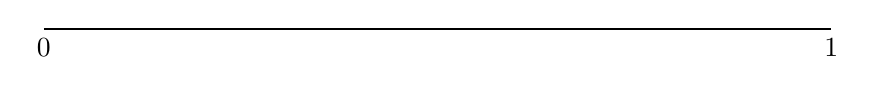
\begin{tikzpicture}
            \draw[thick] (0,0) -- (10,0);
            \node[below] at (0,0) {0};
            \node[below] at (10,0) {1};
        \end{tikzpicture}
    \end{center}

    \item \textbf{Passo 1:} Si rimuove il terzo centrale \(\left( \frac{1}{3}, \frac{2}{3} \right)\).
    
    \begin{center}
        \begin{tikzpicture}
            \draw[thick] (0,0) -- (3,0);
            \draw[thick] (7,0) -- (10,0);
            \node[below] at (0,0) {0};
            \node[below] at (3,0) {$\frac{1}{3}$};
            \node[below] at (7,0) {$\frac{2}{3}$};
            \node[below] at (10,0) {1};
        \end{tikzpicture}
    \end{center}
    
    \item \textbf{Passo 2:} Si rimuovono i terzi centrali da ciascun intervallo rimasto, \(\left( \frac{1}{9}, \frac{2}{9} \right)\) e \(\left( \frac{7}{9}, \frac{8}{9} \right)\).
    
    \begin{center}
        \begin{tikzpicture}
            \draw[thick] (0,0) -- (1,0);
            \draw[thick] (2,0) -- (3,0);
            \draw[thick] (7,0) -- (8,0);
            \draw[thick] (9,0) -- (10,0);
            
            \node[below] at (0,0) {0};
            \node[below] at (1,0) {$\frac{1}{9}$};
            \node[below] at (2,0) {$\frac{2}{9}$};
            \node[below] at (3,0) {$\frac{1}{3}$};
            \node[below] at (7,0) {$\frac{2}{3}$};
            \node[below] at (8,0) {$\frac{7}{9}$};
            \node[below] at (9,0) {$\frac{8}{9}$};
            \node[below] at (10,0) {1};
        \end{tikzpicture}
    \end{center}
    
    \item \textbf{Passi successivi:} Il processo continua indefinitamente, rimuovendo il terzo centrale da ciascun intervallo rimanente.
\end{itemize}
L'insieme che rimane alla fine di questo processo è l'insieme di Cantor.\\
Formalmente, possiamo vedere l'insieme di Canor come l'intersezione numerabile degli insiemi $C^{(i)}$ ottenuti ad ogni passo:
$$C=\bigcap_{n\in \mathbb N} C^{(n)}$$


\begin{figure}[H] % [H] makes sure the figure is placed exactly here
    \centering
    \includegraphics[width=0.4\textwidth]{assets/Three-dimensional-Cantor-set-FMM-tree-for-N-4096-t-1-and-d-H-2-For.png}
    \caption{Polvere di Cantor (Pouransari, Hadi and Darve, Eric, 2015) \cite{article}
}
    \label{fig:example_image}
\end{figure}
\subsubsection{(prop) Proprietà degli insiemi di Cantor}
\begin{enumerate}
    \item $C$ ha la cardinalità del continuo
    \item $C$ ha misura di Lebesgue pari a 0.\\$$\lambda(C)=0$$
    \item $C$ è compatto
    \item $C$ non ha punti interni
    \item $\exists E\subset C$ tale che $E\in \mathcal L(\mathbb R)$ ma $E\notin \mathcal B(\mathbb R)$
\end{enumerate}
\subsection{Funzioni misurabili e integrabili}
\subsubsection{(def) Funzione misurabile}
Siano $(X,\mathcal F)$ e $(Y,\mathcal G)$ due spazi misurabili.\\
Una funzione $f:X\to Y$ viene detta misurabile (o anche $(\mathcal {F,G})$-misurabile) se $$f^{-1}(V)\in \mathcal F\quad \forall V\in\mathcal G$$
\subsubsection{(prop) Condizione necessaria e sufficiente per la misurabilità di una funzione (*)}
Siano $(X,\mathcal F)$ e $(Y,\mathcal G)$ due spazi misurabili.\\
Basta verificare che $f$ soddisfi la definizione di misurabilità per ogni elemento di una famiglia di generatori di $\mathcal G$.\\
Sia $\mathcal S\subset \mathcal G$ tale che $\mathcal G=\sigma_0(\mathcal S)$.\\
Allora vale la seguente doppia implicazione:
$$f \text{ è misurabile}\iff f^{-1}(E)\in \mathcal F\quad  \forall E\in \mathcal S$$
\subsubsection{(def) Borel misurabilità}
Una funzione $f:X\to Y$ si dice Borel misurabile se è $(\mathcal B(X),\mathcal B(Y))$-misurabile.
\subsubsection{(def) Lebesgue misurabilità}
Una funzione $f:X\to Y$ si dice Borel misurabile se è $(\mathcal M,\mathcal B(Y))$-misurabile.\\
Dove $\mathcal M$ è un'insieme che contiene $\mathcal B(X)$, ad esempio:
\begin{itemize}
    \item $\mathcal M=\mathcal B(X)$
    \item $\mathcal M=\mathcal P(X)$
    \item $\mathcal M=\mathcal L(X)$
    \item etc...
\end{itemize}
(oss) Notiamo quindi che la Lebesgue misurabilità implica la Borel misurabilità.
\subsubsection{(prop) continuità e misurabilità di una funzione (*)}
Sia $f:X\to Y$ una funzione continua, allora è anche Borel misurabile e, di conseguenza, Lebesgue misurabile. 
\subsubsection{(prop) misurabilità della composizione di funzioni (*)}
Sia $f:X\to Y$ una funzione Lebesgue misurabile.
Sia $g:Y\to Z$ una funzione continua.
Allora
$$g\circ f:X\to Z$$ è Lebesgue misurabile.
\subsubsection{(prop) misurabilità di una funzione continua su funzioni misurabili (*) }
Date due funzioni $u,v:X\to \mathbb R\ (\text{or }\bar{\mathbb R}) $ tali che $u$ e $v$ siano Lebesgue measurabili.\\
Presa una funzione $\Phi:\mathbb R^2\to \mathbb R$ continua,\\
Allora la funzione $h:X\to \mathbb R$,$$\ h(x)=\Phi(u(x),v(x))$$ è Lebesgue misurabile.
\subsubsection{(def) almost everywhere holding property}
Sia $(X,\mathcal M, \mu)$ uno spazio di misura completo (\ref{(def) completezza della misura o dello spazio di misura}). \\
Una proprietà $P(x)$ è vera per $\mu$-almost every $x\in X$ o $\mu$-almost everywhere (a.e.) se
$$\mu(\{x\in X:P(x)\text{ is false}\})=0$$
\subsubsection{(prop) misurabilità di funzioni uguali a.e.}
\begin{enumerate}
    \item $f:X\to \bar{\mathbb R}$ tale che $f=g$ a.e. , con $g$ misurabile $\implies f$ è misurabile 
    \item Data una successione di funzioni misurabili $\{f_n\}_{n\in \mathbb N}$ tale che $f_n\to f$ a.e. $\implies f$ è misurabile
\end{enumerate}
\newpage

\section{Integrale di Lebesgue}
\chapquote{``I have to pay a certain sum, which I have collected in my pocket. I take the bills and coins out of my pocket and give them to the creditor in the order I find them until I have reached the total sum. This is the Riemann integral. But I can proceed differently. After I have taken all the money out of my pocket I order the bills and coins according to identical values and then I pay the several heaps one after the other to the creditor. This is my integral."}{Henri Lebesgue}

\subsection{Simple Functions}
\subsubsection{(def) Simple and measurable function}
Considerando uno spazio misurabile $(X,\mathcal M)$,\\
$$s:X\to \overline{\mathbb R}$$
è semplice (e misurabile) se:
\begin{itemize}
    \item $s$ è una funzione misurabile
    \item $s(X)=\{a_1,a_2,a_3,\dots,a_k\}$ è un set finito di elementi, dove $a_i\in \overline{\mathbb R}\quad \forall i = 1,\dots, k$ con $a_i\neq a_j$ per ogni $i\neq j$.
\end{itemize}
\textbf{Forma canonica}
$$s(x)=\sum_{i=1}^k a_i\cdot \rchi_{D_i}(x)$$
dove:
\begin{itemize}
    \item $D_i=\{x\in X: s(x)=a_i\}$
    \item $D_i\cap D_j=\emptyset\quad \forall i\neq j$
    \item $X=\bigcup_{i=1}^k D_i$
\end{itemize}
\begin{center}
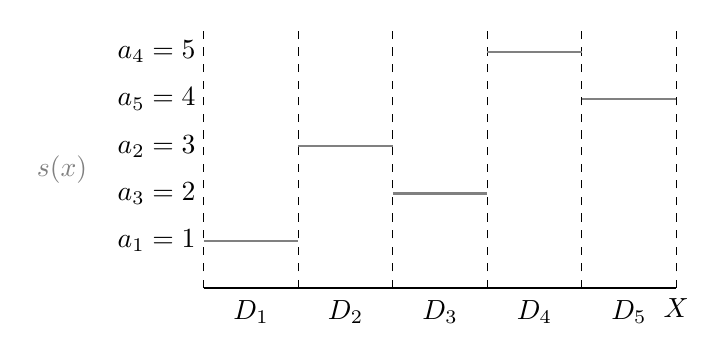
\begin{tikzpicture}[scale=0.6]
    % Define the a_i values
    \def\aone{1}
    \def\atwo{3}
    \def\athree{2}
    \def\afour{5}
    \def\afive{4}
    
    % Define the coordinates for X and D_i sets
    \draw[thick] (0,0) -- (10,0) node[below] {$X$}; % X axis
    \foreach \x in {0, 2, 4, 6, 8, 10} % Vertical lines for D_i sets
        \draw[dashed] (\x,0) -- (\x,5.5);
    
    % Label the D_i sets
    \node at (1,-0.5) {$D_1$};
    \node at (3,-0.5) {$D_2$};
    \node at (5,-0.5) {$D_3$};
    \node at (7,-0.5) {$D_4$};
    \node at (9,-0.5) {$D_5$};
    
    % Plot the values of s(x)
    \draw[thick,gray] (0,\aone) -- (2,\aone); % a_1
    \draw[thick,gray] (2,\atwo) -- (4,\atwo); % a_2
    \draw[thick,gray] (4,\athree) -- (6,\athree); % a_3
    \draw[thick,gray] (6,\afour) -- (8,\afour); % a_4
    \draw[thick,gray] (8,\afive) -- (10,\afive); % a_5
    
    % Label the a_i values
    \node at (-1,\aone) {$a_1=1$};
    \node at (-1,\atwo) {$a_2=3$};
    \node at (-1,\athree) {$a_3=2$};
    \node at (-1,\afour) {$a_4=5$};
    \node at (-1,\afive) {$a_5=4$};

    % y-axis label
    \node[thick, gray] at (-3,2.5) {$s(x)$};

    
\end{tikzpicture}
\end{center}
\subsubsection{(thm) Simple Approximation Theorem (SAT) (*)}
Presi
\begin{itemize}
    \item $(X,\mathcal M)$ spazio misurabile
    \item $f:X\to [0,+\infty]$ funzione misurabile
\end{itemize}
Allora esiste una successione di funzioni semplici misurabili che approssimano dal basso la funzione $f$.
\\ Ovvero:\\
$\exists \{s_n\}_{n\in \mathbb N}$ t.c. $s_i$ è funzione semplice e misurabile $\forall i\in \mathbb N$ e:
$$0\le s_1\le s_2\le \dots \le s_n\le \dots \le f$$ pointwise (ovvero $\forall x \in X$).\\
Si ha quindi che 
$$\lim_{n\to +\infty} s_n(x)=f(x) \quad \forall x\in X$$
Inoltre, se $f$ è bounded, la convergenza è uniforme:
$$\sup_{x\in X}\vert s_n(x)-f(x)\vert \xrightarrow[n\to +\infty]{} 0$$
\subsubsection{(def) Integrale di Lebesgue}
Consideriamo uno spazio di misura $(X,\mathcal M, \mu)$.\\
Sia $s:X\to [0,+\infty]$ una funzione semplice e misurabile:
$$s(x)=\sum_{i=1}^k a_i\cdot \rchi_{D_i}(x)$$
Con $a_i\ge 0$ e $D_i\in \mathcal M$.\\
Sia $E\in \mathcal M$.\\
L'integrale di Lebesgue di $s$ su $E$ è:
$$\int_{E}s\ \mathrm{d\mu}\coloneqq\sum_{i=1}^k a_i\cdot\mu(D_i\cap E)$$

\subsubsection{(prop) Basic properties of the Lebesgue's integral}
Siano $N,E,F\in \mathcal M$, $s_1,s_2:X\to [0,+\infty]$ delle funzioni semplici e misurabili.\\
Allora:\\
\begin{enumerate}
    \item Nullità su insiemi di misura nulla.\\$$\mu(N)=0\implies \int_Ns_1\mathrm{d}\mu=0$$
    \item Omogeneità rispetto alla moltiplicazione per una costante positiva. \\ Data $0\le c\le +\infty $, $$\int_E c\cdot s_1\mathrm{d}\mu=c\int_E s_1\mathrm{d}\mu$$
    \item Additività rispetto alla somma.
    $$\int_E(s_1+s_2)\mathrm{d}\mu=\int_Es_1\mathrm{d}\mu+\int_Es_2\mathrm{d}\mu$$
    \item Monotonicità$$s_1\le s_2\implies \int_Es_1\mathrm{d}\mu\le\int_Es_2\mathrm{d}\mu$$
    \item Monotonia sugli insiemi$$E\subset F\implies \int_Es_1\mathrm{d}\mu\le\int_Fs_1\mathrm d\mu$$ 
\end{enumerate}
\subsubsection{(prop) The integral of non negative simple measurable functions is a measure (*)}
Data $s:X\to[0,+\infty]$, semplice e misurabile,\\
Definendo $\varphi:\mathcal M\to[0,+\infty]$ tale che:
$$\varphi(E)=\int_E s\ \mathrm{d}\mu\quad\text{con } E\in \mathcal M$$
Allora $\varphi$ è una misura su $(X,\mathcal M)$.
\subsubsection{(def) Integrale di funzioni misurabili non negative}
Data una funzione misurabile $f:X\to[0,+\infty]$, $E\in\mathcal M$
$$\int_E f\ \mathrm{d}\mu\coloneqq \sup\Big\{\int_E s\ \mathrm d\mu: s \text{ semplice e misurabile, } 0\le s\le f\Big\}$$
\subsubsection{(prop) Disuguaglianza di Chebyshev (*)}
Considerando: 
\begin{itemize}
    \item uno spazio di misura completo $(X,\mathcal M,\mu)$
    \item $f:X\to[0,+\infty]$, misurabile
    \item $0<c<+\infty$ 
\end{itemize}
Allora
$$\mu\Big(\{x\in X:f(x)\ge c\}\Big)\le\frac1c\int_{\{f\ge c\}}f\ \mathrm{d}\mu \le \frac1c\int_X f\ \mathrm{d}\mu$$
\subsubsection{(lemma) Vanishing lemma (*)}
Dati:
\begin{itemize}
    \item $f:X\to[0,+\infty]$ una funzione misurabile
    \item $E\in\mathcal M$
\end{itemize}
Allora vale:
$$\int_Ef\ \mathrm{d}\mu=0\iff f(x)=0$$ per a.e. $x\in E$
\subsubsection{(lemma) Condizione di finitezza per l'integrale rispetto a una misura (*)}
Data una funzione $f:X\to [0,+\infty]$ misurabile, allora:
$$\int_X f\ \mathrm d\mu<+\infty \iff \mu\Big(\Big\{x\in X:f(x)=+\infty\Big\}\Big)=0$$
\subsection{Convergence Theorems}
\subsubsection{(thm) Monotone Convergence Theorem (Beppo Levi's)}
Given a function $f_n:X\to [0,+\infty]$ measurable $\forall n\in \mathbb N$,\\
Assume:
\begin{enumerate}[label=\roman*.]
    \item $f_n(x)\le f_{n+1}(x)$ for a.e. $x\in X$
    \item $f_n(x)\xrightarrow[n\to+\infty]{} f(x)$ for $\mu$-almost every $x\in X$
\end{enumerate}
Then:
$$\int_X f\ \mathrm d\mu=\lim_{n\to +\infty}\int_X f_n\ \mathrm d\mu$$
Il significato è che presa una successione di funzioni non negative crescente e convergente a una funzione $f$ quasi ovunque, allora l'integrale del limite è pari al limite dell'integrale della successione per $n \to +\infty$

\subsubsection{(corollary) Monotone convergence for series (*)}
Data una funzione $f_n:X\to [0,+\infty]$ misurabile $\forall n\in \mathbb N$
$$\int_X\Big(\sum_{n\in \mathbb N}f_n\Big)\mathrm d\mu=\sum_{n\in\mathbb N}\Big(\int_X f_n \ \mathrm d\mu\Big )$$
\subsubsection{(prop) The integral of a non negative measurable function is a measure (*)}
Presa $\Phi : X\to [0,+\infty]$ misurabile, $E\in \mathcal M$,\\
Si definisce:
$$\nu(E)=\int_E \Phi\ \mathrm d\mu$$
Allora $\nu$ è una misura su $(X,\mathcal M)$,\\
Inoltre (data $f:X\to[0,+\infty]$ misurabile),
$$\int_X f\ \mathrm d\nu = \int_X f\Phi \ \mathrm d\mu$$
\subsubsection{(lemma) Fatou's Lemma (*)}
Considerando:
\begin{itemize}
    \item uno spazio di misura $(X,\mathcal M,\mu)$ completo
    \item $f_n:X\to [0,+\infty]$ misurabile $\forall n\in \mathbb N$
\end{itemize}
Allora:
$$\int_X\Big ( \liminf_n f_n\Big ) \mathrm d\mu\le \liminf_n\Big(\int_X f_n\ \mathrm d\mu\Big)$$
\subsubsection{(def) Funzione integrabile e insieme di funzioni integrabili L1}
$f:X\to \overline{\mathbb R}$ è integrabile su $X$ se:
\begin{itemize}
    \item è misurabile
    \item l'integrale di Lebesgue del modulo della funzione è finito e positivo$$\int_X\vert f\vert \mathrm d\mu <+\infty$$
\end{itemize}
Definiamo quindi
$$\mathcal L^1(X,\mathcal M,\mu)\coloneqq\{f:X\to \overline{\mathbb R}\ |\  f \text{ Lebesgue integrabile}\}$$ 
ovvero l'insieme delle funzioni integrabili secondo Lebesgue.
\subsubsection{(def) integrale di Lebesgue con decomposizione in parti positive e negative}
Per $f\in \mathcal L^1(X,\mathcal M,\mu)$ e $E\in \mathcal M$, definiamo:
$$\int_X f\ \mathrm{d}\mu\coloneqq \int_X f^+\mathrm d\mu-\int_X f^-\mathrm d\mu$$
$$\int_E f\mathrm d\mu \coloneqq \int_X f\rchi_E \mathrm d\mu$$
\subsubsection{(prop) implicazioni della misurabilità (*)}
\begin{enumerate}[label=\roman*]
    \item $f\in \mathcal L^1 \iff |f|\in \mathcal L^1 \iff f^+,f^-\in \mathcal L^1$
    \item triangular inequality $$0\leq \Big\vert\int_X f \mathrm d\mu\Big|\leq \int_X|f|\mathrm d\mu$$
\end{enumerate}
\subsubsection{(prop) $\mathcal L^1$ is a vector space}
\begin{enumerate}
    \item $\mathcal L^1(X,\mathcal M,\mu)$ è uno spazio vettoriale reale
    \item $\int_X \mathrm d\mu:\mathcal L^1(X,\mathcal M,\mu)\to \mathbb R$ è lineare
\end{enumerate}
\subsubsection{(thm) Full optional Vanishing lemma (*)}
Si consideri $(X,\mathcal M,\mu)$ completo, $f,g\in \mathcal L^1(X,\mathcal M,\mu)$.
Allora, $$f=g \text{ a.e. }\iff \int_X |f-g|\mathrm d\mu =0\iff \int_E(f-g)\mathrm d\mu=0\quad \forall E\in \mathcal M$$
\subsubsection{(thm) Lebesgue's Dominated Convergence Theorem}
Sia $(X,\mathcal M,\mu)$ completo.
$\{ f_n\}_{n\in \mathbb N}, \ f_n:X\to \overline{\mathbb R}$ misurabile.

Assumendo:
\begin{itemize}
    \item $f_n(x)\to f(x)$ a.e. $x\in X$
    \item $\exists g\in \mathcal L^1(x)$ tale che $|f_n(x)|\leq g(x)$ a.e. $x\in X$
\end{itemize}
Allora,
$$f\in \mathcal L^1(x) \text{ e }\lim_{n\to +\infty}\int_X|f_n-f|\mathrm d\mu=0$$
$$\lim_{n\to +\infty}\int_Xf_n\mathrm d\mu=\int_X f\mathrm d\mu$$

\subsubsection{(rmk) Dominanted convergence for a.e. bounded functions}
Se $\mu(x)<+\infty \implies$ constants are integrable. Then, if $f_n(x)|\leq M\ a.e.$,
$$\lim_n\int_X f_n=\int_X\lim_n f_n$$
Allora conviene usare semplicemente $g(x) = M$.
\subsubsection{(corollary) Dominated convergence for series}
$\{f_n\}_n\subset \mathcal L^1(X,\mathcal M,\mu)$

Se $\sum_n\int_X |f_n|\mathrm d\mu <+\infty \implies$ $$ \int_X\Big ( \sum_n f_n\Big ) \mathrm d\mu = \sum_n\Big ( \int_X f_n \mathrm d\mu\Big )$$
\subsection{Riemann's vs Lebesgue's integrals}
\subsubsection{(thm) Riemann's proper integrability implies Lebesgue's integrability}
Siano:
\begin{itemize}
    \item $I=[a,b]\subset \mathbb R$
    \item $f:I\to \mathbb R$ Riemann-integrable
\end{itemize}
Allora,
$$f\in \mathcal L^1(I,\mathcal L(I),\lambda)$$
e
$$\int_{[a,b]} f \mathrm d\lambda = \int_a^b f(x) \mathrm dx$$
\subsubsection{(thm) Riemann's $\int_\alpha^\beta|f|\mathrm dx$ (generalized) convergence implications}
Siano $I=(\alpha, \beta)$, $-\infty\leq \alpha <\beta \leq +\infty$\\
Se $|f|$ è Riemann-integrabile in senso generalizzato, allora
\begin{enumerate}
    \item $f \in \mathcal L^1$
    \item $\int_{(\alpha, \beta)} f\mathrm d\lambda = \int_\alpha^\beta f(x)\mathrm dx$
\end{enumerate}
\subsubsection{(rmk) What if $\int_\alpha^\beta|f|\mathrm dx$ (generalized) diverges?}
Se l'integrale di Riemann generalizzato di $|f|$ diverge $\implies \int_{(\alpha,\beta)}|f|\mathrm d\lambda =+\infty$\\
Ma $\int_{(\alpha,\beta)} f\mathrm d\lambda$ non è definito (a meno che $f = \pm |f|$) e $\int_{(\alpha,\beta)} f\mathrm d\lambda $ non è correlato con $\int_\alpha^\beta f(x)\mathrm dx$.\\
\textbf{Example} $f:(0,+\infty)\to \mathbb R$, $f(x)=\frac{\sin x}x$

\section{Spaces of integrable functions}
\subsection{$L^1$ space}
\subsubsection{Da $\mathcal L^1$ a $L^1$}
Consideriamo uno spazio $(X,\mathcal M,\mu)$ completo. \\
Vediamo che:
$$\mathcal L^1(X,\mathcal M,\mu)\coloneqq\{f:X\to \overline{\mathbb R}\ |\  f \text{ Lebesgue integrabile}\}$$
è uno spazio vettoriale. Infatti:
\begin{itemize}
    \item Se $f,g\in \mathcal L^1(E),\ \alpha, \beta \in \mathbb R$\\
     $$\int_E (\alpha f+\beta g)=\alpha \int_E f + \beta \int_E g$$
     \begin{itemize}
         \item $\int_E f\in \mathbb R$
         \item $\int_E g \in \mathbb R$
     \end{itemize}
     $\implies \int_E (\alpha f+\beta g)\in \mathbb R$
\end{itemize}
\paragraph{Ma è uno spazio metrico?}
Uno spazio metrico consente di definire e analizzare la convergenza delle funzioni, inoltre, uno spazio metrico può essere completo (ogni successione di Cauchy converge a un limite all'interno dello spazio). La proprietà di completezza risulta fondamentale in diverse applicazioni che seguiranno, come per le equazioni alle derivate parziali e nella teoria delle distribuzioni.
\paragraph{Ricerca di una distanza in $\mathcal L^1$}

Date due funzioni $f,g\in \mathcal L^1(X,\mathcal M,\mu)$, possiamo definire una distanza $$d_1:\mathcal L^1\times \mathcal L^1\to [0,+\infty), \quad d_1(f,g)=\int_X|f-g|\mathrm \ d\mu$$
(Utilizziamo la norma 1 solo perché lo spazio che stiamo considerando è $\mathcal L^1$, avremmo potuto usare qualsiasi norma, l'indice dello spazio sta a indicare quella utilizzata)\\
Proviamo quindi a verificare che $d_1$ sia effettivamente una distanza, richiamando la definizione (\ref{(def) Metrica (distanza)}):
\begin{enumerate}
    \item $\int_X|f-g|\mathrm \ d\mu=0\iff f=g$\myquad[15] fallisce\\
     $\int_X|f-g|\mathrm \ d\mu\geq 0 \quad \forall f,g\in \mathcal L^1$\myquad[15] ok
    \item $\int_X|f-g|\mathrm \ d\mu=d\int_X|g-f|\mathrm \ d\mu\quad \forall f,g\in \mathcal L^1$\myquad[9] ok
    \item $\int_X|f-g|\mathrm \ d\mu\leq \int_X|f-h|\mathrm \ d\mu+\int_X|h-g|\mathrm \ d\mu\quad \forall f,g,h\in \mathcal L^1$ \quad\  ok
\end{enumerate}
La prima condizione fallisce perché:
\begin{itemize}
    \item $\int_X |f-g|=0\implies f=g$\quad è falso
    \item $\int_X |f-g|=0\impliedby f=g$\quad è vero
\end{itemize}
Osserviamo che è invece vero che $$\int_X |f-g|=0\implies f=g \quad \textbf{a.e.}$$
L'idea a questo punto è quella di modificare lo spazio $\mathcal L^1$, introducendo una classe di equivalenza:
$$u\sim v\iff u(x)=v(x) \text{ for a.e. } x\in X$$
\subsubsection{(def) $L^1$ definition}
Definiamo $L^1$ come:
$$L^1(X,\mathcal M,\mu)\coloneqq \frac{\mathcal L^1(X,\mathcal M,\mu)}\sim =\{[u]\ :\ u\in \mathcal L^1(x)\}$$
Osserviamo che $(L^1, d_1)$ è uno spazio metrico.
\subsection{$L^\infty$ space}
\subsubsection{(def) Essentially bounded functions}
Una funzione si dice essenzialmente limitata se esiste un valore $M$ oltre il quale $f(x)$ può superare $M$ solo su un insieme di misura nulla.

$f:X\to \overline{\mathbb R}$ measurable, it is essentially bounded if $\exists M>0$ s.t. $$\mu(\{x\in X\ :\ |f(x)|>M\})=0$$
In alternativa, $f$ è essentially bounded se $\exists M>0$ tale che $|f(x)|<M $ a.e.
\subsubsection{(def) Essential Supremum ($\esssup$)}
Se $f $ è essentially bounded, l'essential supremum è:
$$\esssup_Xf\coloneqq \inf \left\{ M \in \mathbb{R} : \mu(\{ x \in X : f(x) > M \}) = 0 \right\}$$
Ovvero è il più piccolo numero $M$ tale che la funzione $f(x)$ sia minore o uguale a $M$ su quasi tutto l'insieme $X$, ignorando insiemi di misura nulla.

In altre parole, è il supremo dei valori che la funzione assume quasi ovunque, trascurando eventuali picchi su insiemi trascurabili dal punto di vista della misura.
\subsubsection{(def) $L^\infty$ definition}
$$\mathcal L^\infty(X,\mathcal M,\mu)=\{ f:X\to \overline{\mathbb R}, \text{ essentially bounded}\}$$
$$L^\infty(X,\mathcal M,\mu)=\frac{\mathcal L^\infty(X,\mathcal M,\mu)}\sim$$
Osserviamo che $L^\infty$ è uno spazio vettoriale ed è uno spazio metrico con $d_\infty(f,g)=\esssup_X|u-v|$

\subsection{Tipologie di convergenze}
Vogliamo stabilire se $f_n:X\to \overline{\mathbb R}$, misurabile $\forall n\in \mathbb N$ converge a $f$ per $n\to +\infty$.
\subsubsection{(def) Pointwise convergence}
$$f_n(x)\to f(x)\quad \forall x\in X$$
\subsubsection{(def) Uniform convergence}
$$\sup_X |f_n-f|\to 0$$
\subsubsection{(def) a.e. convergence}
$$f_n(x)\to f(x) \quad \text{for a.e. }x\in X$$
\subsubsection{(def) $L^\infty$-convergence}
$$\esssup_X|f_n-f|\to 0$$
\subsubsection{(def) $L^1$-convergence}
$$\int_X|f_n-f|\mathrm d\mu\to 0$$
\subsubsection{(def) convergence in measure}
$$\forall \alpha>0\quad \mu(\{ x:|f_n-f|\geq \alpha\})\to 0$$
\subsection{Relations between convergences}
\begin{figure}[h]
    \centering
    \includegraphics[width=0.9\linewidth]{assets/convergences_image.png}
    \caption{Convergences relations schema}
    \label{fig:enter-label}
\end{figure}
\begin{itemize}
    \item pointwise convergence $\implies$ a.e. convergence
    \item uniform convergence $\implies$ pointwise convergence
    \item uniform convergence $\implies$ $L^\infty$ convergence
\end{itemize}
\subsubsection{(thm) a.e convergence vs convergence in measure}
Let $\mu(X)<+\infty,\ \{f_n\}_n,\ f$ misurabili e a.e. finite in $X$ ($\vert f\vert<+\infty $ a.e. in $X$ e $\vert f_n\vert<+\infty $ a.e. in $X\quad \forall n$).
$$f_n\to f\text{ a.e. in }X\implies f_n\to f\text{ in measure}$$
\subsubsection{(rkm) Typewriter sequence}
We can see that convergence in measure does not imply a.e. convergence.

\subsubsection{(thm) Convergence in measure implies subsequence a.e. convergence}
Given:
\begin{itemize}
    \item $f_n,\ f$ measurable, a.e. finite
\end{itemize}
If $f_n\to f$ in measure, then $\exists \{f_{n_k}\}_{k\in \mathbb N}$ t.c. $f_{n_k}\to f$ a.e. as $k\to+\infty$\\\\
($\{f_{n_k}\}_{k\in \mathbb N}$ è una sottosequenza di $\{f_n\}_n$)

\subsubsection{(thm) $L^1$ convergence vs convergence in measure (*)}
$f_n,\ f\in L^1(X,\mathcal M,\mu)$ \\
$$f_n\to f\text{ in }L^1,\text{ allora }f_n\to f\text{ in measure}$$
\subsubsection{$L^1$ vs a.e. convergence}
In generale, non sono correlati, ma:
\begin{itemize}
    \item Dominated convergence
    $$\begin{cases}f_n\xrightarrow[]{a.e.} f\\ \exists g\in L^1\quad s.t.\quad |f_n|\leq g \quad a.e.\end{cases}\implies f_n\xrightarrow[]{L^1} f$$
    \item Reverse dominated convergence
    $$f_n\xrightarrow[]{L^1}f \implies \exists \text{ subseq }\{ f_{n_k}\}_k\ :\  \begin{cases}
        f_{n_k}\xrightarrow[]{a.e.}f\\
        \exists g\in L^1\ :\ |f_{n_k}|\leq g\quad a.e.
    \end{cases}$$
\end{itemize}

\section{Teoremi fondamentali del calcolo integrale}
\subsubsection{(recall) Teorema fondamentale del calcolo integrale (Riemann)}
\circled{1}
Se $f\in C([a,b])$, e se definiamo una funzione $F(x)$ come l'integrale definito di $f$ da $a$ a $x$, ovvero:
$$F(x)=\int_a^x f(t)\mathrm dt$$
allora $F(x)\in C^1((a,b))$ e la sua derivata è uguale a $f(x)$:
$$F'(x)=f(x)$$
\circled{2}
Inoltre, se $F$ è una primitiva di $f$ su $[a,b]$, allora
$$\int_a^b f(x)\ \mathrm dx=F(b)-F(a)$$\label{(FFC)}
Ci chiediamo ora cosa succede se $f$ è soltanto $L^1$
\subsection{(thm) 1° Teorema fondamentale del calcolo integrale (*)}
Presi $f\in L^1([a,b]),\ F(x)=\int_a^xf(t)\ \mathrm dt$ allora:
\begin{enumerate}
    \item $F$ è differenziabile in a.e. $x\in [a,b]$
    \item $F'(x)=f(x)$ per a.e. $x\in [a,b]$
\end{enumerate}
\subsubsection{(def) Punto di Lebesgue di $f$}
$f\in \mathcal L^1([a,b]),\ x \in [a,b]$ è un punto di Lebesgue per $f$ se
$$\lim_{h\to 0}\frac 1h \int_x^{x+h}|f(t)-f(x)|\ \mathrm dt=0$$
(se $x=a$, allora $h\to 0^+$, se $x=b$, allora $h\to 0^-$)
\subsubsection{(thm) Lebesgue}
$f\in \mathcal L^1([a,b])\implies $ a.e. $x\in [a,b]$ is a Lebesgue point.
\subsection{Continuity of functions}
\subsubsection{(def) Absolutely Continuous (AC) functions}
Una funzione assolutamente continua ha tutte le proprietà di una funzione continua, ma con qualcosa in più: se scegliamo un gruppo di piccoli intervalli su cui la funzione è definita, la somma dei cambiamenti della funzione su ciascuno di questi intervalli sarà piccola, a patto che la somma delle lunghezze degli intervalli sia piccola.

In altre parole, per una funzione assolutamente continua, possiamo controllare quanto cambia il suo valore “globalmente” spezzando l’intervallo in tante piccole parti: se le parti sono piccole abbastanza, anche i cambiamenti della funzione saranno piccoli.
\paragraph{Formal definition}
$f:I\to \mathbb R$ è una funzione assolutamente continua $f\in AC(I)$ se $\forall \varepsilon>0,\ \exists \delta$ t.c. $\forall n\in \mathbb N$, $\forall$ families of disjoint subintervals of $I$, $\lambda\Big (\bigcup_{i=1}^n(a_i,b_i)\Big )<\delta$
$$\implies \sum_{i=1}^n|f(b_i)-f(a_i)|<\varepsilon$$
\paragraph{Author's remarks}
\begin{itemize}
    \item La composizione di due funzioni assolutamente continue è ancora assolutamente continua, a condizione che una delle funzioni sia limitata.
    \begin{proof}\ 
    
    Take
    \begin{itemize}
        \item $f:[a,b]\to \mathbb R\in AC([a,b])$
        \item $g:\mathbb R\to \mathbb R$, assolutamente continua su ogni intervallo chiuso e limitato
    \end{itemize}
    
    
    \end{proof}
\end{itemize}
\subsubsection{(def) Uniformly Continuous (UC) functions}
$f$ è uniformemente continua se $\forall \varepsilon>0\quad \exists \delta $ t.c., $\forall a_1,b_1\in I$,
$$|a_1-b_1|<\delta \implies |f(a_1)-f(b_1)|<\varepsilon$$
($\delta$ è indipendente da $a_1,b_1$)
$$UC(I)\supset AC(I)$$
\subsubsection{(def) Lipschitz Continuous functions}
If $\exists L>0$ t.c. $\forall x,y\in I$, $|f(x)-f(y)|\leq L|x-y|$
\paragraph{remarks}
\begin{itemize}
    \item The set of Lipschits-continuous functions is strictly contained in the set of AC functions.$$Lip(I)\subset AC(I)$$    
    \item La composizione di funzioni lipschitziane è ancora una funzione lipschitziana.
    \begin{proof}
    Consideriamo due funzioni $f,g\in Lip(I)$,\\
    Per definizione di funzione Lipschitz-continua,
    $\forall\ x,y\in I$:
    \begin{enumerate}
        \item $|f(x)-f(y)|\leq L_1|x-y|$
        \item $|g(x)-g(y)|\leq L_2|x-y|$
    \end{enumerate}
    Di conseguenza,
    $$|f(g(x))-f(g(y)|\leq L_1|g(x)-g(y)|\leq L_1L_2|x-y|$$
    $$L=L_1\cdot L_2$$
    $$\implies f\circ g=f(g(t))\in Lip(I)$$
    
    \end{proof}
\end{itemize}

\subsubsection{(rmk) anticipazione}
Vedremo che
$$Lip(I)\subsetneq  AC(I)\subsetneq  UC(I)$$
Vedremo che:
\begin{itemize}
    \item $g'\in C\iff g\in C^1$
    \item $g'\in L^1\iff g\in AC$
\end{itemize}
\subsection{(thm) 2° Teorema fondamentale del calcolo integrale (*)}
Sia $g:[a,b]\to \mathbb R$. The following propositions are equivalent:
\begin{enumerate}[label=\roman*]
    \item $g$ è assolutamente continua in $[a,b]$ $$g\in AC([a,b])$$
    \item 
    \begin{itemize}
        \item $g$ è differenziabile a.e. in $[a,b]$
        \item $g'\in L^1([a,b])$
        \item $g(x)-g(y)=\int_y^xg'(t)\mathrm dt\quad \forall x,y\in[a,b]$
    \end{itemize}    
\end{enumerate}
\paragraph{Corollary}
$$f\in L^1([a,b])\implies F\in AC([a,b])$$
\subsubsection{(thm) Absolute continuity of the integral (*)}
Let $f\in L^1(X,\mathcal M,\mu)$. Allora $\forall \varepsilon>0\quad \exists \delta>0$ tale che:
$$\begin{cases}
    E\in \mathcal M\\\mu(E)<\delta
\end{cases}\implies \int_E |f| \mathrm d \mu<\varepsilon$$
\subsubsection{(examples) AC not implies Lip continuity}
\textbf{Esempio 1}
Consider $f(x)=\sqrt x $ in $[0,1]$
$$\sqrt x = \int _0^x \frac 1{2\sqrt t }\mathrm dt\quad x\in [0,1]$$
e $g\in AC([0,1])$ (Indeed, $g'\in L^1(0,1)$) 
but $\sqrt{x}\notin $\ Lip\\
\subsubsection{(example) UC does not imply AC}
Considera $$g(x)=\begin{cases}x \sin\frac 1x\quad 0<x\leq 1\\0\quad\quad\quad\quad x=0\end{cases}$$
è continua in $[0,1]\implies g\in UC([0,1])$
But it is not AC.\\
Indeed,
$$ g'(x)=\sin \Big(\frac 1x\Big)-\frac 1x \cos\Big(\frac 1x\Big)\quad 0<x\leq 1$$
\begin{itemize}
    \item $\sin (\frac 1x)\in L^1((0,1))$\\ (si provi applicando il Dominate Convergence Theorem con g=1)
    \item $-\frac 1x \cos(\frac 1x) \notin L^1((0,1))$
\end{itemize}

\subsection{AC functions and weak derivatives}
Lavoriamo in $X=[a,b]\subset \mathbb R$ (diventa molto diverso in $\mathbb R^n$).
\subsubsection{(recall) Compactly supported ($\varphi \in C_0^\infty([a,b])$)}
\begin{itemize}
    \item $\varphi \in C^\infty$
    \item $\exists [c,d]\subset (a,b)$ t.c. $\varphi=0 $ in $ (a,b)\setminus [c,d]$
\end{itemize}
\subsubsection{(prop) intergration by parts in AC}
Take $u\in [a,b]\to \mathbb R$\\
$$u\in AC([a,b])\\\iff$$
\begin{itemize}
    \item $u \in C([a,b])$
    \item u è differenziabile a.e.
    \item $u'\in L^1([a,b])$
    \item $$\int_a^b u'\varphi \mathrm d x = -\int_a^b u\varphi'\mathrm d x\quad \forall \varphi \in C_0^\infty([a,b])$$
\end{itemize}

\subsubsection{(def) $W^{1,1}(a,b)$ Weak derivative}
Let $u\in L^1(a,b)$. \\
Diciamo che $$u \in W^{1,1}(a,b) \iff \exists w\in L^1(a,b) \text{ t.c. } \int_a^b u\varphi '\mathrm dx=-\int_a^b w\varphi \mathrm d x \quad \forall \varphi \in C_0^\infty $$

Such a $w$ is called weak derivative of $u$ in $(a,b)$, denoted $u'$
\subsubsection{(rmk) Remarks on weak derivatives}
\paragraph{rmk 0)}
\begin{itemize}
    \item $C([a,b])\iff L^1(a,b)$
    \item $C^1([a,b])\iff W^{1,1}(a,b)$
\end{itemize}
\paragraph{rmk 1)}
Both $u$ and $w=u'$ are equivalence classes
\paragraph{rmk 2)}
If such a $w$ exists, it is unique.
$$\int_a^b u \varphi ' = -\int_a^b w_1\varphi $$
$$\int_a^b u \varphi ' = -\int_a^b w_2\varphi $$
$\forall \varphi \in C_0^\infty ([a,b])$
$$\implies\int_a^b(w_1-w_2)\varphi =0\quad \forall \varphi \in C_0^\infty$$
$$\implies w_1-w_2=0\quad a.e. \text{ in} \ [a,b]$$
\paragraph{rmk 3)}
In principle, the pointwise and weak derivatives are different objects, and the notation $u'$ may be misleading.\\
But we know that if we take absolute continuous functions, they coincide.
\paragraph{rmk 4)}
The definition of weak derivative can be extended in the senses of measures, of distributions.

Take $$H(x)=\begin{cases} 0\quad x<0\\ 1\quad x>0\end{cases}$$
$$-\int_{-1}^1 H(x)\varphi '(x)\mathrm d x = -\int_0^1 \varphi'(x)\mathrm d x = -\varphi(1)+\varphi(0)$$
$$\varphi(1)=0$$

$$\varphi(0)=\int_{[-1,1]} \varphi \mathrm\ d\delta_0$$
This suggests that $H^1$ è pari a 0 almost everywhere (pointwise), ma è pari a $\delta_0$ (dirac) weakly
\subsubsection{(thm) AC and $W^{1,1}$ relation (*)}
$$u\in  AC([a,b])\iff u \in W^{1,1}([a,b])$$

\section{Derivatives of measures}
Consider $(X,\mathcal M,\mu)$ complete measure space.\\
We know that, given $\Phi :X\to [0,+\infty]$ measurable, the function
$$\nu_\Phi(E) \coloneqq \int_E \Phi \ \mathrm d\mu=\int_E \mathrm d\nu_\Phi$$
is a measure on $(X,\mathcal M)$.
\subsubsection{(def) Radon-Nikodin derivative (density for $\nu$ w.r.t. $\mu$)}
Consider $\mu, \nu$ measures on $(X,\mathcal M)$. If 
$$\exists\ \Phi \text{ s.t. } \nu(E)=\int_E \Phi\ \mathrm d\mu\quad \forall E\in \mathcal M$$
Then $\Phi$ is the Radon-Nikodym derivative of $\nu$ w.r.t. $\mu$:
$$\Phi = \frac{\mathrm d\nu}{\mathrm d\mu}$$
$\Phi:X\to[0,+\infty]$ acts as density for $\nu$ w.r.t. $\mu$, if fact, it expresses $\nu$ in terms of $\mu$ through the integral.
\subsubsection{(def) Absolute Continuous (AC) Measures}
Given $\mu, \nu$ measures on $(X,\mathcal M)$.\\
Then $\nu$ è assolutamente continua w.r.t. $\mu$ (notazione: $\nu << \mu$) se, 
$$\forall E \in \mathcal M,\ \mu(E)=0\implies \nu(E)=0$$
\subsubsection{(lemma) Absolute Continuity Lemma via Density Function 
 (*)}
$$\exists\ \Phi \text{ s.t. }\nu(E)=\int_E \Phi\ \mathrm d\mu\quad \forall E\in \mathcal M\implies \nu<<\mu$$
So the existance of the Radon-Nikodym derivative implies the absolute continuity of $\nu$ w.r.t. $\mu$.
\begin{proof}
 This holds because if $\nu(E)=\int_E\Phi\ \mathrm d\mu$ for all measurable sets $E$, then:
\begin{itemize}
    \item Whenever $\mu(E)=0$, the integral $\int_E \Phi \ \mathrm d\mu$ must also be zero because there is "no mass" in $E$ w.r.t. $\mu$. Consequently, $\nu(E)=0$ as well.
    \item This means that $\nu(E)=0$ whenever $\mu(E)=0$, which is precisely the definition of absolute continuity of $\nu$ w.r.t. $\mu$.
\end{itemize}   
\end{proof}


\subsubsection{(thm) Radon-Nikodym Theorem}
Consider:
\begin{itemize}
    \item $(X,\mathcal M)$ measurable space,
    \item $\mu, \nu$ measures,
    \item $\mu$ is $\sigma -$finite
\end{itemize}
Then:
$$\nu<<\mu\iff \exists\frac{\mathrm d \nu}{\mathrm d\mu}$$
\paragraph{Corollary} \ \\
$\nu$ measure on $(\mathbb R^n,\mathcal L(\mathbb R^n))$ and $\nu<<\lambda\implies$
$$\exists\ \Phi : \nu(E)=\int_E \Phi\ \mathrm d\lambda \quad \forall E\in \mathcal L(\mathbb R^n)$$
(Indeed, $\lambda $ is $\sigma-$finite)

\section{Functional Analysis Introduction - Banach Spaces}
\chapquote{``A mathematician is a person who can find analogies between theorems; a better mathematician is one who can see analogies between proofs and the best mathematician can notice analogies between theories."}{Stefan Banach}

\begin{center}
    "infinite dimension linear algebra"
\end{center}

Take $X$ vector space.
$$\text{dim}(X)=N<+\infty \implies X\simeq \mathbb R^n$$

Typical examples of $X:\text{dim} (X)=+\infty$ are "function spaces".

\paragraph{Typical applications} Differential Equations. All them from an abstract point of view, can be seen as problem in functional spaces.

\paragraph{Example}
$$-\Delta : C^2(\Omega ) \to C(\Omega)$$
Then $-\Delta u = f$ is a linear problem in $\infty$-dimension, as well as $A\bar x = \bar b$ is a linear problem in finite dimension.
\subsection{Basic definitions}
\subsubsection{(def) Norm on X}
A norm on X is a function:
$$\Vert \cdot\Vert :X\to \mathbb R$$
such that:
\begin{enumerate}
    \item $\Vert x\Vert \geq 0\quad \forall x\in X,\ \Vert x\Vert =0\iff x=0$
    \item $\Vert \alpha x \Vert = |\alpha|\cdot \Vert x\Vert\quad \forall \alpha \in \mathbb R, x\in X$\
    \item $\Vert x+y \Vert \leq \Vert x\Vert + \Vert y\Vert \quad x,y\in X$\tab (Triangular inequality)
\end{enumerate}
\subsubsection{(def) Normed space}
$X$ is called normed (vector) space if:
\begin{itemize}
    \item $X$ has a vector space structure
    \item We can do linear combinations of the vectors in out space:\\
    Given $v,w\in X,\ \alpha,\beta\in \mathbb R\implies$
    $$\alpha v+\beta w\in X$$
    \item has a norm $\cnorm$ defined on it
\end{itemize}
The normed vector space is denoted as $(X,\cnorm)$.
\subsubsection{(prop) "normed" implies "metric" space}
Take $(X,\Vert \cdot \Vert )$ normed, we can choose $$d(x,y)=\Vert x-y\Vert$$
Then $d$ is a distance on $X\implies (X,d)$ is a metric space.

Questo vuol dire che ogni spazio normato è anche uno spazio metrico.
\subsubsection{(rmk) Topologia normica}
Definire una norma su uno spazio vettoriale induce una distanza, che a sua volta induce una topologia sullo spazio.

La distanza $d$ induce una topologia su $X$, chiamata topologia indotta dalla norma o topologia normica. In questa topologia, un insieme $Y\subset X$ è aperto se, per ogni punto $x_0\in Y$, esiste un $r>0$ tale che la palla aperta di raggio $r$ centrata in $x_0$,
$$B_r(x_0)=\{x\in Y:d(x,x_0)<r\}$$
è contenuta in $Y$.
\subsubsection{(prop) caratterizzazione sequenziale della continuità per funzioni tra spazi normati}
 $f:X\to Y$ ($X,Y$ spazi normati),
    $$f\text{ is continuous at }x \iff \forall \{x_n\}_n:x_n\to x \text{ in } X \text{ it holds } f(x_n)\to f(x) \text{ in } Y$$
Questa proprietà permette di verificare la continuità di $f$ tramite la convergenza delle successioni piuttosto che tramite la definizione $\varepsilon\text-\delta$
\paragraph{Definizione $\varepsilon$-$\delta$ di continuità}
 $f:X\to Y$ ($X,Y$ spazi metrici), afferma che $f$ è continua in un punto $x\in X$ se:
 $$\forall \varepsilon, \ \exists\delta >0 \text{ t.c. }d_X(x,x_0)<\delta \implies d_Y(f(x),f(x_0))<\varepsilon \quad \forall x_0\in X$$

\subsubsection{(def) Convergenza forte (convergenza nella norma)}
Consideriamo $X$ normed space.\\
Una successione $\{x_n\}_{n\in \mathbb N}\subset X$ in uno spazio normato $X$ converge a $x\in X$ se la distanza (misurata nella norma) tra $x_n$ e $x$ tende a zero al tendere di $n$ all'infinito.
$$\Vert x_n-x\Vert\xrightarrow[n\to+\infty]{}0$$
\subsubsection{Exercises}
Show that:
\begin{enumerate}
    \item $$\Big \vert \Vert x\Vert -\Vert y\Vert \Big \vert \leq \Vert x-y\Vert $$
    \item $$\Vert \cdot \Vert :X\to \mathbb R$$ is continuous in $X$
\end{enumerate}
\subsubsection{(def) Cauchy sequence}
$\{x_n\}_n\subset X$ is a Cauchy sequence (or fundamental sequence) if 
$$\Vert x_n-x_m\Vert \to 0\quad \text{as }n,m\to +\infty$$
($\forall \varepsilon>0 \quad \exists \bar n \ : \ n,m\geq \bar n \implies \Vert x_n-x_m\Vert \leq \varepsilon$)
\paragraph{(rmk) Cauchy sequences does not always converge}
$$\{ x_n\}_n \text{ converges }\substack{\implies\\ \centernot\impliedby} \{x_n\}_n \text{ is Cauchy sequence} $$

\subsection{Equivalent and Non-equivalet norms}
\subsubsection{(def) Equivalent norm}
Take a vector space $X$, and take two norms:
\begin{itemize}
    \item $\Vert\cdot \Vert _a: X\to \mathbb R$
    \item $\Vert\cdot \Vert _b: X\to \mathbb R$
\end{itemize}
they are equivalent if $\exists\ 0<c_1\leq c_2$ such that:
$$c_1\Vert x\Vert_a\leq \Vert x\Vert_b\leq c_2 \Vert x\Vert _a$$
(in particular, they induce the same convergence, topology, ...)

In $\mathbb R^n$ every norm is equivalent to every other norm...
\subsubsection{(thm) Norms equivalence theorem}
Take a vector space $X$, $\text{dim}(X)<+\infty$.

Then all norms are equivalent.

\begin{proof}\ \\
\begin{enumerate}
    \item it is enough to check that any norm $\Vert \cdot \Vert$ is equivalent to $\cnorm$ is equivalent to $\cnorm_2$.
    \item If $\cnorm$ is any norm, $\exists c_1, c_2>0 \text{ s.t. } 0<c_1\leq \Vert x\Vert \leq c_1\quad \forall x\in X:\Vert x\Vert_2=1$
    \item $f(x)=\Vert x\Vert$, $f:\mathbb R^n\to \mathbb R$
We want to show that $f$ is continuous with respect to the Euclidean norm $\cnorm_2:$\\
$$\Vert x_n-x\Vert_2\xrightarrow[n\to +\infty]{}0\implies f(x_n-x)\to 0$$
$$\Vert x_n-x\Vert \to 0$$
\end{enumerate}
Indeed, take any vector $y\in X$ with ($e_1,\dots,e_n)$ basis of $X$
$$\Vert y\Vert=\Big\Vert\sum_{i=1}^n y_ie_i\Big\Vert$$
By the triangular inequality,
$$\Big\Vert\sum_{i=1}^n y_ie_i\Big\Vert\leq \sum_{i=1}^n\Vert y_ie_i\Vert\leq\sum_{i=1}^n|y_i|\Vert e_i\Vert$$
$$\leq \Big (\max_{i=1,\dots,n}|y_i|\Big)\cdot \sum_{i=1}^n\Vert e_i\Vert$$
Name $C=\sum_{i=1}^n\Vert e_i\Vert$
$$=C\Vert y\Vert_\infty\leq C \Vert y\Vert_2$$
Then
$$0\leq \Vert x_n-x\Vert\leq C\Vert x_1-x\Vert_2\to 0$$
Consider the problem:
$$\min_{\Vert x\Vert_2=1}f(x),\max_{\Vert x\Vert_2=1}f(x)$$
Since $f$ is continuous and $\{ x:\Vert x\Vert_2 =1$ is compact.
Thanks to Weierstrass, we know that the sup and inf exists, and so there are two point $x_m, x_M\in \partial B_1(0)$ such that:
$$\Vert x_m\Vert\leq \Vert x\Vert \leq \Vert x_M\Vert$$
Since $\Vert x_m\Vert_2=1\implies x_m\neq 0$
$$0<\Vert x_m\Vert\leq \Vert x\Vert \leq \Vert x_M\Vert$$
\end{proof}

\subsection{Banach spaces} %rivedere definizione
$(X,\Vert\cdot \Vert )$ normed vector space is a Banach space if it is complete, i.e. every Cauchy sequence converges in $X$.
\paragraph{Examples}
\begin{itemize}
    \item $(\mathbb R^n,\Vert x\Vert_p)$, with:
    $$\Vert x\Vert_p\coloneqq\begin{cases}
        \Vert x\Vert_p=\Big (\sum_{i=
    1}^N|x_i|^p\Big )^{\frac 1p}\quad 1\leq p<+\infty\\
    \Vert x\Vert_\infty=\max_i|x_i|
    \end{cases}$$

 is a Banach space (e.g. $p=2$ "Euclidean norm" which comes from a scalar product).
 \item $\Big(C([a,b]),\ \Vert u\Vert _{C([a,b])}\Big)$, with:
 $$\Vert u\Vert _{C([a,b])}=\max _{[a,b]}|u|$$ is a Banach space.
 \item $\Big (C^k([a,b]), \ \Vert u\Vert_{C^k([a,b])} \Big)\quad k\geq 1$
 , with:
 $$\Vert u\Vert_{C^k([a,b])}=\sum_{i=0}^k \Vert u^{(i)}\Vert_{C([a,b])}$$ is Banach.
\end{itemize}
By now, $L^1,L^\infty, \mathrm{Lip}([a,b]), W^{(1,1)}, AC([a,b])$ are Banach spaces with the right norm.
\paragraph{(rmk) Sequence convergence in Banach space}\ \\
Consider a normed space $(X,\Vert\cdot \Vert)$ and $\{x_n\}_n\subset X$.
We can define a series in terms of its partial sums 
 ($s_k$), and we say that the series converges to some element $y\in X$ if the sequence of partial sums $\{s_k\}_{k\in \mathbb N}$ converges to $y$ in the norm:
$$\sum_{n=1}^{+\infty} x_n=y\iff s_k=\sum_{n=1}^kx_n$$
$$\quad \quad \quad \quad \quad \quad \quad\ \  s_k\xrightarrow[k\to +\infty]{} y$$
In the context of real numbers, we have numerical series: $\{a_n\}_n\subset \mathbb R$ and we can apply the absolute convergence theorem, that guarantees the convergence of the series in $\mathbb R$
$$\sum_{n=1}^{+\infty}|a_n|<+\infty\implies \sum_{n=1}^{+\infty} a_n \text{ converges}$$
This property does not hold in general normed space $(X,\cnorm)$: $\sum_{n=1}^{+\infty}\Vert x_n\Vert <+\infty$ does not imply that $\sum_{n=1}^{+\infty}$ converges in $X$. This is due to the lack of completeness in some normed spaces or the possibility that elements in the sequence $\{x_n\}$ do not "line up" in a way that would allow their partial sums to converge to a limit in $X$.

To guarantee the convergence, we need additional structure, such as $X$ begin a Banach space (see the folloing proposition).
\subsubsection{(prop) Absolute Convergence of series in Banach spaces}
$$(X,\Vert\cdot\Vert) \text{ is Banach space}\iff \begin{cases}\forall \{x_n\}_n\subset X\\ \sum_{n=1}^\infty \Vert x_n\Vert <+\infty\end{cases}\implies \sum_{n=1}^\infty x_n \text{ converges}$$
\section{Lebesgue's spaces}
Consider $(X,\mathcal M,\mu)$ a complete measure space. $p\in [1,+\infty]$

We already defined the $L^1$ and $L^\infty$ of $X$. Analogously, we treat $1\leq p<+\infty$.
\begin{enumerate}
    \item $$\mathcal L^p(X,\mathcal M,\mu)\coloneqq \{u:X\to\overline{\mathbb R}, \text{ measurable, } \int_X |u|^p\ \mathrm d\mu<+\infty\}$$
    
    Remember that the integral is always definite since $u$ is measurable.
    \item $$u,v\in \mathcal L^p(X),\quad u\sim v\iff u(x)=v(x) \text{ for a.e. } x\in X$$
    \item $$L^p(X,\mathcal M,\mu)=\frac{\mathcal L^p(X,\mathcal M,\mu)}\sim$$
    \item $$\Vert u\Vert_{L^p(X)}=\Vert u\Vert_p=\begin{cases}\Big (\int_X |u|^p\ \mathrm d\mu \Big )^{\frac{1}{p}}\quad 1\leq p<+\infty\\ \esssup_X|u|\quad \quad \quad p=+\infty\end{cases}$$
    (and $d_p(f,g)=\Vert f-g\Vert_p$)
\end{enumerate}
\paragraph{Examples}
\begin{enumerate}
    \item Think $X$ as $\mathbb R^n$ with $n\geq 1$,\\
    Let's define omega as a subset of $X$:
    $$\Omega\subset \mathbb R^n$$
$$\Omega \in \mathcal L(\mathbb R^n)$$
So we have:
$$\mathcal M=\mathcal L(X),\ \mu=\lambda \ \ (\Omega =(a,b))$$
\item Take now $(X,\mathcal M,\mu)=(\mathbb N, \mathcal P(\mathbb N), \mu_\#)$\\ \ \\
This means that:
$$\ell^p\coloneqq L^p(\mathbb N, \mathcal P(\mathbb N), \mu_\#)$$
$$\ell^p\coloneqq \begin{cases}
    \Big\{x=(x_k)_{k\in\mathbb N}\ : \ \sum_{k\in \mathbb N}|x_k|^p<+\infty\Big\}\quad 1\leq p<+\infty\\
    \Big\{ x=(x_k)_{k\in \mathbb N}: \sup_{\mathbb N}|x_k|<+\infty\Big\}\quad \quad\ \  p=+\infty
\end{cases}$$
With norm 
$$\Vert x\Vert_{\ell^p}=\begin{cases}
    \Big (\sum_{k\in \mathbb N}|x_k|^p\Big)^{\frac 1p} \quad 1\leq p<+\infty\\
    \sup_{\mathbb N}|x_k| \quad \quad \quad \quad p=+\infty
\end{cases}$$

\end{enumerate}

\paragraph{Plan} Show that $L^p(X),\ 1\leq p\leq +\infty$ are Banach space.
We have to show that:
\begin{enumerate}
    \item $L^p(X)$ is a vector space
    \item $(L^p(X),\cnorm_p)$ is a normed vector space
    \item $(L^p(X),\cnorm_p)$ is a complete normed vector space (Banach space)
\end{enumerate}
To prove each step, we will need to introduce few theorems, lemmas and propositions.
\subsection{$L^p(X)$ is a vector space}
\subsubsection{(lemma) Power Mean Inequality}
$$p\in [1,+\infty), \ a,b\in \mathbb R, \ a,b\geq 0 \implies (a+b)^p\leq 2^{p-1}(a^p+b^p)$$
Proof: exercise (hint: consider cases $a=0$ and $a\neq 0, \ t=\frac ba$)
\subsubsection{(proof) $L^p(X)$ is a vector space}
Assume $1\leq p< +\infty$ ($+\infty$ has different proof procedure, do it as an exercise).
\\ \ \\
Take $u,v\in X$, $\alpha\in\mathbb R$, we have to show that:
\begin{enumerate}
    \item $\alpha u\in L^p(X)$
    \item $u+v\in L^p(X)$
\end{enumerate}
\begin{proof}\ 
\begin{enumerate}
    \item $$0\leq \int_X|\alpha u|^p\mathrm d\mu=|\alpha|^p\int_X |u|^p\mathrm d\mu <+\infty$$
(if $u$ is measurable $\implies |u|$ is measurable non negative and $0\leq \int_X|u|^p\mathrm d\mu\leq +\infty$ is well defined).
\item $$\int_X|u+v|^p\mathrm d\mu\leq \int_X\Big(|u|+|v|\Big)^p\mathrm d\mu\leq 2^{p-1}\int_X\Big ( |u|^p+|v|^p\Big ) \mathrm d\mu=$$
$$=2^{p-1}\Big [\int_X |u|^p\mathrm d\mu +\int_X |v|^p\mathrm d\mu\Big]$$
\end{enumerate}
\end{proof}

\subsection{$(L^p(X),\cnorm_p)$ is a normed vector space}
I have to show that $\cnorm_p$ is a norm in $L^p(X)$. Also here we'll consider cases where $1\leq p< +\infty$, the case $+\infty$ is given as exercise to the reader.
\\\ \\
We have to show:

\begin{enumerate}
    \item 
        \begin{enumerate}[label=(\alph*)]
            \item $\Vert u\Vert_p\geq 0 \quad \forall u \in L^p(X)$
            \item $\Vert u\Vert_p=0\iff u=0\ \text{in} \ L^p(X)$
        \end{enumerate}
    \item $\Vert \alpha u \Vert_p=|\alpha |\Vert u\Vert_p $
    \item Triangular inequality
\end{enumerate}
\subsubsection{(def) Conjugate exponent}
Given every $1\leq p\leq +\infty$, the conjugate exponent (sometimes denoted as $p'\in [1,+\infty]$) satisfies:
$$\frac 1p +\frac 1{p'}=1$$
\begin{itemize}
    \item $(p')'=p$
    \item $ p=1\iff p'=+\infty$
    \item $p+p'=pp'$
    \item $p'(p-1)=p$
    \item $p'=\frac p{p-1}$
\end{itemize}

\subsubsection{(lemma) Young inequality}
$1<p<+\infty$, $a,b\in \mathbb R$, $a,b\geq 0$\\
Then:
$$ab\leq \frac 1p a^p+\frac 1{p'} b^{p'}$$
\begin{proof}
Remember what a concave function is...\\
$f \text{ concave},\ 0\leq \lambda\leq 1$
$$f((1-\lambda)x+\lambda y)\geq (1-\lambda)f(x)+\lambda f(y)$$
Apply to 
\begin{itemize}
    \item $f(x)=\ln x$
    \item $x=a^p$
    \item $y=b^{p'}$
    \item $\lambda = \frac 1{p'}$
    \item $1-\lambda = \frac 1p$
\end{itemize}
$$\ln\Big(\frac 1p a^p+\frac 1{p'} b^{p'}\Big)\geq \frac 1p \ln(a^p)+\frac 1{p'}\ln(b^{p'})=\dots=\ln(ab)$$
\end{proof}
\paragraph{Consequences}
Hölder's inequality
\subsubsection{(thm) Hölder's inequality (*)}
Given:
\begin{itemize}
    \item $(X, \mathcal M,\mu)$ complete measure space.
    \item $u,v$ measurable
    \item $1\leq p,p'\leq +\infty$
    \item $\frac 1p +\frac 1{p'}=1$
\end{itemize}
Then, $$\Vert uv\Vert_1 \leq \Vert u\Vert_p\Vert v\Vert_{p'}$$
\begin{proof} \ \\
    Firstly, consider $1<p,p'<+\infty$
    \begin{itemize}
        \item If $\Vert u\Vert_p =0$ (or respectively, $\Vert v\Vert_{p'}=0$) then $u=0$ a.e. (respectively, $v=0$ a.e.)
    $$\implies uv=0 \ a.e.$$
    $$\implies \Vert uv\Vert_1 =0$$
    \item If $\Vert u\Vert_p\neq0, \ \Vert v\Vert_{p'}\neq 0$ and $\Vert u\Vert_p\cdot \Vert v\Vert_{p'}=+\infty\implies$ the inequality holds.
    \item Finally, if $0<\Vert u\Vert_p, \ \Vert v\Vert_{p'}<+\infty$\\
    We can apply Young inequality to $a=\frac{|u(x)|}{\Vert u\Vert_p}, b =\frac{|v(x)|}{\Vert v\Vert_{p'}}$:
    $$\frac{|u(x)|\cdot |v(x)|}{\Vert u\Vert_p\Vert v\Vert_{p'}}=ab\leq \frac 1p \frac{|u(x)|^p}{\Vert u\Vert_p^p}+\frac 1{p'}\frac{|v(x)|^{p'}}{\Vert v\Vert_p^{p'}}$$
    Integrating,
    $$\frac{\Vert uv\Vert_1}{\Vert u\Vert_p\Vert v\Vert_{p'}}\leq \frac{1}{p}\frac{\Vert u\Vert_p^p}{\Vert u\Vert_p^p}+\frac 1{p'}\frac{\Vert v\Vert_{p'}^{p'}}{\Vert v\Vert_{p'}^{p'}}=1$$
    \paragraph{Exercise}
    Conclude the proof with cases $p=1, p'=+\infty$
    \end{itemize}
\end{proof}
\subsubsection{(thm) Minkowski inequality (*)}
Take $(X,\mathcal M,\mu)$ a complete measure space, $1\leq p\leq +\infty$\\
Then, $\forall u,v\in L^p(X)$
$$\Vert u+v\Vert_p\leq \Vert u\Vert_p+\Vert v\Vert_p$$
\begin{proof}\ \\
    Let's start considering the case $1<p<\infty$
    $$\Vert u+v\Vert_p^p=\int_X|u+v|^p\ \mathrm d\mu =$$
    $$= \int_X |u+v|\cdot |u+v|^{p-1}\ \mathrm d\mu\leq \int_X |u|\cdot |u+v|^{p-1}\ \mathrm d\mu +\int_X|v|\cdot |u+v|^{p-1}\ \mathrm d\mu$$
    \begin{itemize}
        \item We can estimate $\int_X |u|\cdot |u+v|^{p-1}\ \mathrm d\mu $ \\ Thanks to Hölder inequality:
    $$\int_X |u|\cdot |u+v|^{p-1}\ \mathrm d\mu \leq \Big (\int_X |u|^p\ \mathrm d\mu \Big)^{\frac 1p}\Big ( \int_X |u+v|^{(p-1)p'}\mathrm d\mu\Big)^{\frac 1{p'}}$$
    Recalling $(p-1)p'=p$,
    $$\int_X |u|\cdot |u+v|^{p-1}\ \mathrm d\mu \leq \Vert u \Vert_p\Vert u+v\Vert_p^{p/p'}=\Vert u\Vert_p\Vert u+v\Vert_p^{p-1}$$
    \item Analogously, we can estimate $\int_X|v|\cdot |u+v|^{p-1}\ \mathrm d\mu$, obtaining:
    $$\int_X|v|\cdot |u+v|^{p-1}\ \mathrm d\mu\leq \Vert v\Vert_p\Vert u+v\Vert_p^{p-1}$$
    \end{itemize}
    Reassembling all the terms in the inequality,
    $$\Vert u+v\Vert_p^p\leq \Vert u\Vert_p\Vert u+v\Vert_p^{p-1}+\Vert v\Vert_p\Vert u+v\Vert_p^{p-1}$$
    Eventually, dividing by $\Vert v\Vert_p\Vert u+v\Vert_p^{p-1}$, we obtain the Minkowski inequality.

    \paragraph{Exercise} Proofs for cases $p=1$ and $p=+\infty$ are given as an exercise to the reader
    
\end{proof}
\subsubsection{(proof) $(L^p(X),\cnorm_p)$ is a normed vector space}
\begin{proof}\ 
\begin{enumerate}
    \item 
        \begin{enumerate}[label=(\alph*)]
            \item $\Vert u\Vert_p\geq 0 \quad \forall u \in L^p(X)$\\
            $\to$ Since $\Vert u\Vert_p=\Big (\int_X|u(x)|^p\ \mathrm dx\Big )^{\frac 1p}$ and the absolute value of $u(x)$ is always positive $\forall x\in X$, we can say that $\Vert u\Vert _p$ is always positive $\forall u \in L^p(X)$
            \item $\Vert u\Vert_p=0\iff u=0\ \text{in} \ L^p(X)$\\
            $\to$ Trivial
        \end{enumerate}
    \item $\Vert \alpha u \Vert_p=|\alpha |\Vert u\Vert_p $\\
    $\to$ We have: $$\Vert \alpha u\Vert_p=\Big (\int_X|\alpha u(x)|^p\ \mathrm dx\Big )^{\frac 1p}$$
    $$\Vert \alpha u\Vert_p=\Big (\int_X|\alpha|^p|u(x)|^p\ \mathrm dx\Big )^{\frac 1p}$$
    $$\Vert \alpha u\Vert_p=|\alpha|\Big (\int_X|u(x)|^p\ \mathrm dx\Big )^{\frac 1p}$$
    $$\Vert \alpha u\Vert_p=|\alpha |\Vert u\Vert_p $$
    \item Triangular inequality $\to$ Minkowski inequality
\end{enumerate}
\end{proof}

\subsection{Completeness of $L^p(X,\mathcal M,\mu)$}
\subsubsection{(thm) Riesz-Fischer}
Consider $(X,\mathcal{M},\mu)$ a complete measure space, with $1\leq p\leq +\infty$.\\
Then, $L^p(X,\mathcal M,\mu)$ is a Banach space.
\begin{proof}\ \\
    We already proved that $L^p$ is a normed vector space, the only missing property is completeness. We will use the characterization of Banach spaces in terms of absolutely converging series.\\
    $L^p(X)$ is Banach $\iff \forall \{f_n\}_n\subseteq L^p(X)$
    $$\sum_{n=1}^{+\infty}\Vert f_n\Vert_p<+\infty\implies \sum_{n=1}^{+\infty} f_n \text{ converges in }L^p(X)$$
    Introduce $g_k(x)=\sum_{n=1}^k|f_n(x)|$ (measurable)\\
            $$\forall x\in X, g_k(x)\nearrow$$
$$\implies g(x)=\lim_{k\to +\infty}g_k(x)=\sum_{n=1}^{+\infty}|f_n(x)|\leq +\infty$$
    Then, using Minkowsky inequality: 
    $$\Vert g_k\Vert_{L^p}=\Big \Vert\sum_{n=1}^k|f_n(x)| \Big\Vert\leq \sum_{n=1}^k\Vert f_n\Vert_p\leq\sum_{n=1}^{+\infty}\Vert f_n\Vert_p=M<+\infty$$
    That is, $g_k\in L^p(X)$\\
    Then, 
    $$\int_X|g|^p\mathrm d\mu=\int_X|\lim_k g_k|^p\mathrm d\mu$$
    By the Monotone Convergence Theorem:
    $$\lim_k\int_X|g_k|^p\mathrm d\mu=\lim_k\Vert g_k\Vert_p^p\leq M^p<+\infty$$
    Then $g\in L^p(X)\implies g(x)<+\infty$ for a.e. $x$
    $$\sum_{n=1}^{+\infty} |f_n(x)|<+\infty\text{ for a.e. }x$$
    $$\implies \sum_{n=1}^{+\infty}f_n(x)\text{ converges for a.e. }x$$
    $$s(x)=\sum_{n=1}^{+\infty}f_n(x)\text{ is well defined (a.e.) and }s_k(x)\to s(x) \text{ for a.e. }x\in X$$
    To conclude, we apply the Dominated Convergence Theorem.
    \begin{itemize}
        \item $|s_k(x)-s(x)|^p\to 0\quad a.e.$
        \item $|s_k-s|^p=\Big |\sum_{n=1}^kf_n-\sum_{n=1}^{+\infty}f_n\Big |^p = \Big(\Big |\sum_{n=k+1}^{+\infty}f_n\Big|\Big)^p\leq\Big (\sum_{n=k+1}^{+\infty}|f_n|\Big )^p\leq (g)^p\in L^1$
    \end{itemize}    
    Resuming:
    $$\begin{cases}
        |s_k-s|^p\to0\text{ a.e.}\\
        |s_k-s|^p\leq g^p\in L^1(X)
    \end{cases}\substack{D.C.T.\\ \implies} \int_X |s_k-s|^p\mathrm d\mu\to 0$$
 that is, convergence in $L^p$
    
\end{proof}
\subsection{Inclusion of $L^p$ spaces}
\subsubsection{(thm) Embedding Theorem for $L^q$ into $L^p$ ($\mu(X)<+\infty$)}
Take a measurable space $(X,\mathcal M,\mu)$, with:
\begin{itemize}
    \item $\mu(X)<+\infty$
    \item $1\leq p\leq q\leq +\infty$
\end{itemize}
Then $$L^q(X)\subset L^p(X)$$
This result is based on the fact that when the measure of the space $X$ is finite, integrability for a larger exponent $q$ implies integrability for any smaller exponent $p$. \\
More precisely, $\exists\ C>0 \ : \Vert u\Vert_p \leq C\Vert u\Vert_q$
\subsubsection{(thm) Interpolation Inequality (*)}
If $1\leq p<q\leq +\infty$
$$L^r(X)\subset L^p(X)\cap L^q(X)\quad \forall p\leq r\leq q$$
\begin{proof}\ 
\begin{enumerate}
    \item Let $f\in L^p(X)$ and $q<+\infty$\\
Then, $$\int_X |f|^p\mathrm d\mu=\int_X |f|^p\cdot 1\ \mathrm d\mu \leq \Big (\int_X |f|^q\mathrm d\mu\Big )^{\frac pq}\Big (\int_X 1\ \mathrm d\mu\Big)^{\frac{q-p}{p}}$$
$\frac pq\in (0,1)$ so we can apply the Hölder's inequality with $\frac qp\implies \frac pq + \frac{q-p}{q}=1$\\
That's equal to $\mu(X)^{\frac qp}\Vert f\Vert_q^p$
$$\implies \Vert f\Vert_p\leq \mu(X)^{q-p}\Vert f\Vert_q$$
Let $f\in L^\infty(X)$,
$$\Big ( \int |f|^p\mathrm d\mu\Big )^{\frac{1}{p}}\leq \Vert f\Vert_\infty \Big (\int_X1\mathrm d\mu\Big)^{\frac 1p}=\Vert f\Vert_\infty \mu(X)^{\frac 1p}$$
In conclusion 
$$\Vert f\Vert_p\leq \mu(X)^p\Vert f\Vert_\infty$$
\item Suppose $q = +\infty$\\
If $r\in (p,q) $
$$\exists \ t\in (0,1)\text{ s.t. }\quad r=tp+(1-t)q $$
Hence
$$\Vert f\Vert_r^r =\int_X|f(x)|^r\mathrm d\mu =\int_X|f(x)|^{tp}\Vert f(x)\Vert^{(1-t)q}\mathrm d\mu$$
$$\leq \Big (\int_X|f|^p\mathrm d \mu\Big )^t\Big (\int_X |f|^q\mathrm d\mu\Big )^{1-t}=\Vert f\Vert_p^{tp}\Vert f\Vert_q^{(1-t)q}$$
Applying Hölder's inequality,
$$\Vert f\Vert_r\leq \Vert f\Vert_p^{\frac{tp}{r}}\Vert f\Vert_q^{\frac{(1-t)q}{r}}$$
\item Suppose $q=+\infty$, let $r>p$
$$\Vert f\Vert_r^r =\int_X|f(x)|^r\mathrm d\mu =\int_X |f|^{r-p}|f|^p\leq \Vert f\Vert_\infty^{r-p}\int_X|f(x)|^p\mathrm d\mu=\Vert f\Vert_p^p$$
$$\implies \Vert f\Vert_r\leq \Vert f\Vert_\infty^{\frac{r-p}{r}}\Vert f\Vert^{\frac pr}$$

\end{enumerate}


\end{proof}
\subsection{Back to general theory of Banach spaces}
We know that the following are Banach:
\begin{itemize}
    \item $(\mathbb R^n,\text{ any norm})$
    \item $(L^p(X),\cnorm_p)$
    \item $(L^\infty(X),\cnorm_\infty)$
    \item $(C(X),\cnorm_\infty)$
\end{itemize}
Differences between finite/infinite dimensional spaces
\begin{center}
    \begin{table}[h]
        \begin{tabular}{lll}
        \hline
                         & finite ($\dim(X)<+\infty$)         & infinite ($\dim(X)=+\infty$) \\ \hline
        Completeness     & always                            & not always                  \\
        Equivalent norms & all                               & not all                     \\
        Compactness      & compact $\iff$ closed and bounded & no                          \\
        Density          &                                   &                            \\\hline
        \end{tabular}
\end{table}
\end{center}

\subsubsection{Example}
$X=C([-1,1])$ with norm $\Vert u\Vert_1=\int_{-1}^1|u(x)|\mathrm dx$
$$u_n(x)=\begin{cases}
    0\quad x\leq0\\nx\quad 0\leq x\leq \frac 1n\\1\quad x\geq \frac 1n
\end{cases}$$
$u_n\in X\quad \forall n\geq 1$\\
Show that $\{u_n\}$ is a Cauchy sequence with respect to $\cnorm_1$ ($m>n$)
$$0\leq \Vert u_n-u_m\Vert_1=$$
$$=\int_{-1}^1|u_n(x)-u_m(x)|\mathrm dx=\int_{-1}^00\mathrm dx+\int_0^{\frac 1m}(mx-nx)\mathrm dx+\int_{\frac 1m}^{\frac 1n}(1-nx)\mathrm dx+\int_{\frac 1n}^1(1-1)\mathrm dx= $$
$$= \dots = \frac{m-n}{2m^2}+\frac{(1-\frac nm)^2}{2n}\leq \frac 1{2m}+\frac 1{2n}\xrightarrow[m,n\to 0]{}0$$
On the other hand:
$$\Vert u_n-u_m\Vert_\infty=\max_{-1\leq x\leq 1}|u_n(X)-u_m(x)|=1-\frac nm\centernot\to0\text{ as }n,m\to +\infty$$
Moreover $\{u_n\}\subset L^1([-1,1])$
\paragraph{Exercise}
Show that $u_n\to \mathcal H$ (Heaviside)
\paragraph{Consequences}
\begin{enumerate}
    \item $\cnorm_1$ and $\cnorm_\infty$ are not equivalent in $C([-1,1])$
    \item $(C([-1,1]),\cnorm_1)$ is not a Banach space ($\mathcal H\notin C([-1,1])$
    \item $X=L^1([-1,1])$\\ $V=C([-1,1])$\\$V\subset X$ is a vector subspace
    $$\begin{cases}
        \{u_n\}_n\subset V\\ u_n\to \mathcal H \text{ in } X
    \end{cases} \text{ but }\mathcal H\notin V$$
    that is, $V$ is not closed.
    "find the element of $V$ which best approximates $\mathcal H$ in $X$". $dist(\mathcal H,V)=0$, but there is no point at minimal distance.
\end{enumerate}
\subsubsection{(rmk) Closed subsets/subspaces}
Considering $(X,d)$ a metric space,
\begin{itemize}
    \item $C\subset X$ is closed $\iff$ $\partial C\subset C$ ($\overline C=C$)
\end{itemize}
    from the sequential point of view:
    \begin{itemize}
        \item $C\subset X$ is closed $\iff$
    $$\begin{cases}
        \{ x_n\}_n\subset C\\ x_n\to y\in X
    \end{cases}\implies y\in C$$
    \end{itemize}
    
\paragraph{Properties of closed subspaces}
\begin{enumerate}
    \item Completeness: In a Banach space, every closed subspace is itself a Banach space with the induced norm.
\end{enumerate}
\section{Compactness}
$E\subset X$ is compact if from any open covering $\{ A_i\}_{i\in I}$ ($A_i$ open $\forall i\in I$, $E\subset \bigcup_{i\in I}A_i$) we can extract a finite subcovering.\\
Typically, we can take $E$, fix $r>0$, consider $\{ B_r(x)\}_{x\in E}$. Then $$E\subset \bigcup_{x\in E}B_r(x)$$
If $E$ is compact, $\exists x_1,x_2,\dots, x_k\in E$ s.t. $$E\subset \bigcup_{i=1}^k B_r(x_i)$$
\subsubsection{(def) Sequentially compact}
$E$ is sequentially compact if $\forall \{x_n\}_{n\in \mathbb N}\subset E$,
$$\exists \{ x_{n_k}\} \text{ convergent in }E$$
\subsubsection{(def) Relatively compact set}
$E\subset X$ is relatively compact if $\overline E$ is compact
\subsection{Finite dimension}
\subsubsection{(thm) Heine-Borel}
Consider $(X,\cnorm )$ a normed vector space. If $\dim (X)<+\infty$,
$$E \text{ compact }\iff E \text{ closed and bounded}$$
\paragraph{Remark}
If $\dim(X)=+\infty$,
$$E\text{ compact}\substack{\implies\\ \centernot\impliedby} E\text{ closed and bounded}$$
\subsection{Infinite dimension}
\subsubsection{(thm) Riesz}
Take any normed vector space $(X,\cnorm)$, \\
take the ball of radius 1 and centered in origin $$\overline{B_1(0)}\text{ is compact }\iff \dim(X)<+\infty$$
\begin{proof}\ \\
$\impliedby$: see analysis 1,2 + equivalent norms\\
$\implies$: assume that $\overline{B_1(0)}=\{ x\in X: \Vert x\Vert \leq 1\}$ is compact.\\
Consider $\{B_{\frac 12}(x)\}_{x\in \overline{B_1(0)}}$\\
($B_{\frac 12}(x)=\{y\in X:\Vert x-y\Vert <\frac 12\}$)\\
Then $$\overline{B_1(0)}\subset \bigcup_{x\in \overline{B_1(0)}}B_{\frac 12}(x)$$
By compactness, $\exists\ x_1,x_2,\dots,x_k\in \overline{B_1(0)}$ s.t.
$$\overline{B_1(0)}\subset \bigcup_{i=1}^kB_{\frac 12}(x_i)\subset \bigcup_{i=1}^k\overline{B_{\frac 12}(x_i)}$$
This means that:
    $$\forall x\in \overline{B_1(0)}\quad \exists\ i\in \{1,\dots,k\},\quad \exists \ z:\Vert z\Vert \leq \frac 12\quad \text{ s.t. }x=x_i+z$$
Define $V=span\{x_1,\dots,x_n\}$ \\
Then $V\subset X$ is a vector subspace and $dim(V)\leq k<+\infty$\\
Then we can rewrite:
$$\forall x\in \overline{B_1(0)}\quad \exists\ v\in V,\quad \exists \ z\in X:\Vert z\Vert \leq \frac 12\quad \text{ s.t. }x=v+z$$
Take $y\in X(y\neq0)\implies \frac{y}{\Vert y\Vert}\in \overline{B_1(0)}$ and $\exists v\in V, \ z:\Vert z\Vert \leq \frac 12$ s.t. 
$$\frac y{\Vert y\Vert}=v+z$$
i.e.
$$y=v\Vert y\Vert+z\Vert y\Vert $$
Defining $v'\coloneqq v\Vert y\Vert$, $z'\coloneqq z\Vert y\Vert$,
$$y=v'+z'$$
where $v'\in V, \ \Vert z'\Vert \leq \frac{\Vert y\Vert}{2}$\\
Take any $x\in X$, apply the last result to $y=x$.
$$x=v_1+z_1$$
where $v_1\in V, \ \Vert z_1\Vert \leq \frac{\Vert x\Vert}2$.\\
apply again, to $y=z_1$\\
$$x=v_1+v'+z'$$
$v'\in V$, $\Vert z'\Vert \leq \frac{z_1}2\leq \frac{\Vert x\Vert}4$\\
$v_2 = v_1+v'$, $z'=z_2$\\
$$x =v_2+z_2$$
$$v_2\in V, \ \Vert z_2\Vert \leq \frac 14 \Vert x\Vert$$
By induction, ...
$$x=v_n+z_n$$
where $v_n\in V, \ \Vert z_n\Vert \leq \frac 1{2^n}\Vert x\Vert$\\
Then:
$$z_n\xrightarrow[n\to+\infty]{}0$$
$$v_n=x-z_n\xrightarrow[n\to+\infty]{}x$$
$$\begin{cases}
    \{v_n\}\subset V\\v_n\to x\in X
\end{cases}\implies x\in V$$
$$dim(V)<+\infty\implies V\text{ is closed}$$
I have shown that $$\forall x\in X\implies x\in V$$
i.e. $X=V$ and $dim (X)\leq k<+\infty$
\end{proof}
\subsection{Compactness in $C([a,b])$}
We always consider $(C([a,b]),\cnorm_\infty)$ which is a Banach space.
$$\Vert u\Vert_\infty =\max_{x\in [a,b]}|u(x)|$$
(one may deal with $C(Q)$ with $Q\subset \mathbb R^n$ closed and bounded).
\subsubsection{(def) Uniform Equicontinuity of a sequence}
Take $\{u_n\}_{n\in \mathbb N}\subset C([a,b])$ is uniformly equicontinuous if $$\forall \varepsilon>0,\ \exists\ \delta >0 \text{ s.t. }|x-y|<\delta$$ 
$$\implies |u_n(x)-u_n(y)|<\varepsilon\quad \forall x,y\in [a,b], \ \forall n\in \mathbb N$$
This means that every functions $u_n$ in the sequence behaves similarly in terms of continuitym with the same $\delta$ working for all functions in the sequence, not just for a specific function.

\paragraph{remarks}
\begin{itemize}
    \item In the pointwise continuity definition of $u$ in $x_0$, we have:
    $$ \delta = \delta(u,x_0,\varepsilon)$$
    \item In the uniform continuity definition of $u$, we have:
    $$ \delta = \delta(u,\varepsilon)$$
    \item In the uniform equicontinuity of $\{u\}_n$ we have:
    $$\delta = \delta(\varepsilon)$$
\end{itemize}
This progression from pointwise continuity to uniform continuity reflects increasing uniformity in the way continuity is controlled across different functions and points.
\subsubsection{(thm) Ascoli-Arzelà}
Take $\{u_n\}_{n\in \mathbb N}\subset C([a,b])$.\\
Assume:
\begin{itemize}
    \item $\{u_n\}_{n\in \mathbb N}$ is unif. bounded
    $$\Vert u_n\Vert_\infty\leq M\quad\forall n$$
    \item $\{u_n\}_{n\in \mathbb N}$ unif. equicontinuous
\end{itemize}
Then:\\
$\exists$ a subsequence $\{u_{n_k}\}_{k\in \mathbb N}$ and $u\in C([a,b])$ s.t. $u_{n_k}\xrightarrow[k\to+\infty]{}u$
\paragraph{Example} $\{u_n\}\subset C^1([a,b])\subset C([a,b])$.\\
Assume that
\begin{enumerate}
    \item $\Vert u_n\Vert_\infty \leq M\quad \forall n$
    \item $\Vert u'_n\Vert_\infty\leq L\quad \forall n$
\end{enumerate}
(for some constants $M,L\geq 0$)\\
Then the theorem applies. Indeed:
\begin{enumerate}
    \item $\implies$ i) in Ascoli-Arzelà thm.
\end{enumerate}
To check equicontinuity: $\forall x,y\in[a,b], \quad x\neq y$
$$|u_n(x)-u_n(y)|=|u'_n(\xi)\cdot (x-y)|$$
(by Lagrange mean value theorem, $\xi$ in the smaller interval)
$$|u_n(x)-u_n(y)|\leq|u'_n(\xi)|\cdot|x-y|\leq \Vert u'_n\Vert_\infty\cdot|x-y|\leq L|x-y|\quad ,\forall n$$
$\implies$ Equicontinuity: $\forall \varepsilon $ take $\delta =\frac \varepsilon L$
Roughly:
$$\text{"boundedness in }C^1\implies \text{ compactness in }C^0\text{"} $$
\paragraph{rmk}
The same is true for Lipschitz continuous functions with uniformly bounded Lipschitz constant
\paragraph{rmk}
there are similar theorems in $L^p, \dots W^{1,p}$
$$\text{"boundedness in }W^{1,p}\implies \text{ compactness in }L^p\text{"} $$
\subsection{Density, Separability}
$(X,d)$ metric space.
\subsubsection{(def) dense space}
$D\subset X$ is dense if $\overline{D}=X$ ($\forall x\in X\quad \exists \{y_n\}_n\subset D : \ y_n\to x\text{ in }X$)
\subsubsection{(def) separable space}
$X$ is separable if $\exists D\subset X$, $D$ countable and dense.
\paragraph{rmk} tipically, one uses dense subsets because "continuous properties, true on $D$, are true in $X$".\\
When $D$ is separable, you have few elements to check the property.
\paragraph{Example}
$\mathbb R,\ \mathbb R^n,\ \Omega \subset \mathbb R^n$ are all separable: $\overline{\mathbb Q}=\mathbb R$ and $\mathbb Q$ is countable.
\subsubsection{(thm) Separability of functional spaces ($C,\ L^p, L^\infty$)} %thm??? maybe a remark...
\begin{itemize}
    \item $(C([a,b]), \cnorm_\infty)$ is separable
    \item $(L^p(\mathbb R), \cnorm_p)$ is separable if $1\leq p<+\infty$
    \item $(L^\infty(\mathbb R),\cnorm_\infty)$ is not separable
\end{itemize}
\subsubsection{(thm) Stone-Weierstrass}
"Polynomials" are dense in $C([a,b])$
(and polynomials with coefficients in $\mathbb Q$ are countable and dense)
\paragraph{Alternative statement (Wikipedia)}
Also known as "Weierstrass approximation theorem", states that every continuous function defined on a closed interval $[a,b]$ can be uniformly approximated as closely as desired by a polynomial function.
\paragraph{Explaination}
The functions belonging to $C([a,b])$ take real values in the interval $[a,b]$ and are equipped with the sup norm ($\cnorm_\infty$ norm): $$\Vert f-g\Vert =\sup_{x\in [a,b]}|f(x)-g(x)|$$
this norm measures the maximum difference between two functions over the interval $[a,b]$. 

Saying that polynomials are dense in $C([a,b])$ means that for any continuous function $f\in C([a,b])$ and any given $\varepsilon>0$, there exists a polynomial $p(x)$ s.t. $$\Vert f-p\Vert <\varepsilon$$.
\subsection{Dense subspaces of $L^p(\mathbb R)$}
\paragraph{Recall}
$s$ is (measurable and) simple function \\$s:\mathbb R\to\mathbb R$ s.t.
$$s=\sum_{i=1}^ka_i\rchi_{E_i}$$
where
\begin{itemize}
    \item $a_i\in \mathbb R$ (distinct)
    \item $E_i\in \mathcal L(\mathbb R)$ (disjoint)
    \item $\bigcup E_i=\mathbb R$
\end{itemize}
We know that $s$ simple $\implies$ $s \in L^\infty(\mathbb R)$
\paragraph{Question}
Does $s\in L^p(\mathbb R)$ (with $1\leq p<+\infty$)?
\paragraph{Answer}
$$s\in L^p(\mathbb R)\iff \lambda\Big (\{x:s(x)\neq0\}\Big)<+\infty$$
$\tilde{\mathcal S}(\mathbb  R)\coloneqq\lambda\Big (\{x:s(x)\neq0\}\Big)$
\subsubsection{(thm) $\tilde S(\mathbb R)$ is dense in $L^p(\mathbb R)$}
$\tilde{\mathcal S}(\mathbb R)$ is dense in $L^p(\mathbb R)\quad \forall \ 1\leq p<+\infty$

\subsubsection{(def) support}
\begin{itemize}
    \item $u:\mathbb R\to \mathbb R$. The support of $u$ is $$supp(u)=\overline{\{x\in \mathbb R : \ u(x)\neq 0}$$
    \item $C_c(\mathbb R)=\{ u\in C(\mathbb R): \ supp(u)$ is compact$\}$
    \item $C_c^\infty(\mathbb R)=C_0^\infty(\mathbb R)=\mathcal D(\mathbb R)$
\end{itemize}
\subsubsection{(thm) $C_c^\infty$ density in $L^p(\mathbb R)$}
$C_c^\infty(\mathbb R)$ is dense in $L^p(\mathbb R)$ $\forall\ 1\leq p<+\infty$\\
By consequence, also $C_c(\mathbb R)$ is dense, etc.
\subsubsection{(rmk) $C_c(\mathbb R)$ is not dense in $L^\infty(\mathbb R)$}
$C_c(\mathbb R)\subset L^\infty(\mathbb R)$ is not dense (i.e. the space of continuous function with compact support in $\mathbb R$ is not dense in the space of essentially bounded functions).

Saying that $C_c(\mathbb R)$ is dense in $L^\infty(\mathbb R)$ would mean that any function in $L^\infty(\mathbb R)$ could be approximated arbitrarily closely (in the $\cnorm_\infty$ norm) by functions from $C_c(\mathbb R)$.


Take
$$\mathcal H(x) =\begin{cases}
    1\quad x\geq0\\0\quad x<0
\end{cases}$$
We observe that $\mathcal H(x)$ is clearly a function $\in L^\infty(\mathbb R)$ since it can be bounded with $\Vert\mathcal H\Vert_\infty=1$.\\
Suppose now to pick a function $g\in C_c(\mathbb R)$ s.t. $\Vert \mathcal H-g\Vert_\infty \leq \frac 13$ (i.e. $| \mathcal H-g| \leq \frac 13$ a.e. $x\in \mathbb R$)

$$\mathcal H(x)-\frac{1}{3}\leq g\leq \mathcal H(x)+\frac 13\quad , \forall x\in \mathbb R$$
\begin{figure}[h]
    \centering
    \includegraphics[width=0.9\linewidth]{assets/heaviside_cartoon.png}
    \caption{Graph of $\mathcal H(x)$ and $g(x)$}
    \label{fig:enter-label}
\end{figure}

We immidiately notice that $g$ can't be a continuous function in $x=0$, since the left-hand and the right-hand limits doesn't agree.\\
$\implies \ g$ $\mathcal H(x)$ can't be approximated arbitrarily closely in $\cnorm_\infty$-norm by any $g\in C_c(\mathbb R)$. Thus, $C_c(\mathbb R)$ is not dense in $L^\infty(\mathbb R)$.

\subsubsection{(lemma) Non-separable Banach spaces}
Take any $X$ Banach space (assumption may be restricted, we use Banach for simplicity)\\
Assume that $\{A_i\}_{i\in I}$ is s.t.
\begin{itemize}
    \item $\forall i\in I,\ A_i\subset X$ open, non empty
    \item $A_i\cap A_j=\emptyset\quad \forall i\neq j$
    \item $I$ is more than countable
\end{itemize}
Then $X$ is not separable
\begin{proof}
    By contradiction, assume $X$ separable, and so there is a countable dense subset $\{x_n\}$ of $X$:
    $$\exists\ \{x_n\}_{n\in \mathbb N}\subset X\text{ s.t. } X=\overline{\bigcup_{n\in \mathbb N}\{x_n\}}$$
    
    $\forall A_i \ ,\exists\ x_{n(i)}\in A_i$
    \begin{enumerate}
        \item $A_i$ not empty $\implies \exists\ z_i\in A_i$
        \item $\{x_n\}$ dense $\implies x_{n_k}\to z_i$
        \item $A_i$ open $\implies$ the sequence enters $A_i$
    \end{enumerate}
    Since $A_i\cap A_j=\emptyset \quad \forall i\neq j$
    then $x_{n(i)}\neq x_{n(j)}$ i.e. $n(i)\neq n(j)$\\
    We have a map
    $$I\in i \xrightarrow[\quad\quad]{}n(i)\in \mathbb N$$ is injective
    $\implies I$ is at most countable, contradiction
\end{proof}
\subsubsection{(thm) $L^\infty(\mathbb R)$ is not separable}
\begin{proof}
    We use the above lemma.\\
    $\forall \alpha\in \mathbb R^+=(0,+\infty)$\\
    $\alpha_1\quad -\alpha_1\quad \alpha_2\quad -\alpha_2$
    take $$g_\alpha (x)=\rchi_{[-\alpha, \alpha]}(x)=\begin{cases}
        1\quad |x|\leq \alpha \\
        0\quad |x|>\alpha
    \end{cases}$$
$$\alpha_1\neq \alpha_2 \implies \Vert g_{\alpha_1}-g_{\alpha_2}\Vert_\infty=1$$

\begin{figure}[H]
    \centering
    \includegraphics[width=0.5\linewidth]{assets/g_alpha1&2.png}
    \caption{$\Vert g_{\alpha_1}-g_{\alpha_2}\Vert_{\infty}=1$ (orange segment)}
    \label{fig:enter-label}
\end{figure}
$\implies B_{1/2}(g_{\alpha_1})\cap B_{1/2}(g_{\alpha_2})=\emptyset $
\begin{figure}[H]
    \centering
    \includegraphics[width=0.3\linewidth]{assets/12balls_in_g_alpha.png}
    \label{fig:enter-label}
\end{figure}
$\forall f\in L^\infty(\mathbb R)$,\\
$$1=\Vert g_{\alpha_1}-g_{\alpha_2}\Vert_\infty\leq \Vert g_{\alpha_1}-f\Vert_\infty +\Vert f-g_{\alpha_2}\Vert_\infty$$ one of them is $>\frac 12$
Then we can apply the lemma using $\{B_{\frac12}(g_\alpha)\}_{\alpha\in (0,+\infty)}$ since it is:
\begin{itemize}
    \item Open
    \item Non-empty
    \item Disjoint
    \item $(0,+\infty)$ is more than countable
\end{itemize}
\end{proof}

\section{Linear Operators}
Consider $(X,\cnorm_X), (Y,\cnorm_Y)$ normed spaces (or just take Banach). \\
$T:X\to Y$ is a \textbf{linear} operator (or linear map) if
\begin{itemize}
    \item $T(\alpha u +\beta v)=\alpha T(u)+\beta T(v)\quad \forall u,v\in X\quad \forall \alpha,\beta \in \mathbb R$
\end{itemize}
If $Y=\mathbb R$, we usually call the linear operators as "\textbf{linear functionals}".
\paragraph{Notation}
$T$ linear, $T(u)=Tu$
\paragraph{Example}
Let's consider $X=\mathbb R^n,\ Y=\mathbb R^m$ and
$$T:\mathbb R^n\to \mathbb R^m \text{ linear}$$
With such spaces, the operator is just a matrix $A\in \mathbb R^{m\times n}$, which means that:
$$T \vec{u}=A \vec{u}$$
In infinite-dimensional spaces (like function spaces), linear operators cannot be usually represented by matrices directly, but similar ideas hold.
\paragraph{Remark}
$$T\text{ linear}\implies T(0)=0$$
\subsubsection{(def) Bounded linear operator}
$T:X\to Y$ linear is bounded if
$$\exists M>0 \text{ s.t. }\Vert Tu\Vert _Y\leq M\Vert u\Vert _X\quad ,\forall u\in X$$
\paragraph{Recall}
\begin{itemize}
    \item $T$ is Lipschitz continuous  $\iff\exists L>0$ s.t. $\Vert Tu-Tv\Vert_Y\leq L\Vert u-v\Vert _X$
    \item $T$ is continuous at $u_0\in X \iff \forall u_n\to u_0\implies T u_n\to T u_0$
\end{itemize}
\paragraph{Remark}
In finite dimensions, any linear map $T:\mathbb R^n\to\mathbb R^m$, $m,n<+\infty$ is both continuous and bounded ($\Vert A\vec x\Vert_2\leq \Vert A\Vert _2\Vert \vec x\Vert _2$).
\paragraph{Fact} if $X,Y$ are $\infty$-dimensional,
\begin{itemize}
    \item linearity $\centernot\implies $ continuity
    \item linearity $\centernot \implies $ boundedness
\end{itemize}
When $X$ and $Y$ are infinite-dimensional, we can’t generally assume that a linear map between them will be continuous or bounded. The existence of such maps is often a non-constructive result provided by the Axiom of Choice, meaning that while we know these maps exist, we can’t necessarily construct explicit examples.
\subsubsection{(thm) Bounded Linear Operator Theorem}
$T:X\to Y$ linear. The following propositions are equivalent:
\begin{enumerate}
    \item $T$ is bounded
    \item $T$ is Lipschitz continuous
    \item $T$ is continuous at any $x_0\in X$
    \item $T$ is continuous at $0$
\end{enumerate}
\begin{proof}\
    \begin{itemize}
        \item  1)$\implies$2) \\$T \text{ bounded}\iff \Vert Tx\Vert _Y\leq M\Vert x\Vert _X\quad \forall x\in X$\\ take $x=u-v$
        $$\Vert T(u-v)\Vert_Y\leq M\Vert u-v\Vert _X$$
        $$\Vert Tu-Tv\Vert_Y\leq M\Vert u-v\Vert _X$$
        that is Lipschitz continuity (by taking $L=M$).
        \item 2)$\implies$3) \\
        We have to check if our operator is continuous, so we ask ourselves: "Does $x_n\to x_0$ imply $Tx_n\to Tx_0$?"\\
        From the definition of norm and Lipschitz continuity of an operator, we can deduce the following inequality:
        $$0\leq\Vert Tx_n-T x_0\Vert_Y \leq L\Vert x_n-x_0\Vert_X$$
        Now we notice that if $x_n\to x_0$ then $L\Vert x_n-x_0\Vert_X\to 0$, and so, from the inequality above, $\Vert Tx_n-T x_0\Vert_Y=0 \implies Tx_n\to Tx_0$.
        \item 3)$\implies$4) $\to $ trivial.
        \item 4)$\implies$1)\\
        By contradiction, assume that $T$ is not bounded (for any constant, we have a vector that give us the opposite inequality):
        $$\forall n\in \mathbb N\quad \exists\ x_n\in X\ : \ \Vert Tx_n\Vert_Y\geq n\Vert x_n\Vert _X \quad (\circledast_1)$$
        Let $$z_n= \frac 1n\frac{x_n}{\Vert x_n\Vert_X}$$
        Then 
        $$\Vert z_n\Vert _X=\frac 1n\xrightarrow[n\to+\infty]{} 0\implies Tz_n \xrightarrow[n\to+\infty]{}T_0=0 \text{ in }Y$$
        But $$(\circledast_1)\implies \Vert Tz_n\Vert_Y=\Big\Vert T\Big(\frac 1n \frac{x_n}{\Vert x_n\Vert_X}\Big)\Big\Vert_Y=\frac{1}{n\Vert x_n\Vert_X}\Vert T x_n\Vert_Y\geq 1 \not \to 0$$
        contradiction
        
    \end{itemize}
\end{proof}
\subsubsection{(def) Space of Bounded Linear Operators / Dual Space}
$$\mathcal L(X,Y)\coloneqq \Big\{ T:X\to Y \text{ s.t. } T \text{ is linear and continuous}\Big\}$$
\paragraph{Notation}
\begin{itemize}
    \item If $Y=X$, one writes $\mathcal L(X)$
    \item If $Y=\mathbb R$ then $\mathcal L(X,\mathbb R)=$"dual of $X$"=$X^*=X'$
\end{itemize}
\paragraph{Remark}
\begin{itemize}
    \item $\mathcal L(X,Y)$ is a vector space: $T,L\in \mathcal L(X,Y)$
    $$(\alpha T+\beta L)(x)\coloneqq \alpha Tx+\beta Lx$$
    $(\alpha T+\beta L)\in\mathcal L(X,Y)$
    \item We define a norm on $\mathcal L(X,Y)$ (operator norm)
    $$\Vert T\Vert_{\mathcal L(X,Y)}=\sup_{\Vert x\Vert \leq 1}\Vert Tx\Vert _Y$$
    (Check that this is a norm)
\end{itemize}
\subsubsection{(prop) Operator norm}
$$\Vert T\Vert_{\mathcal L(X,Y)}=\sup_{\Vert x\Vert =1}\Vert Tx\Vert_Y=\sup_{x\neq 0}\frac{\Vert Tx\Vert _Y}{\Vert x\Vert _X}=$$
$$=\inf\Big\{M>0:\Vert Tx\Vert_Y\leq M\Vert x\Vert _Y\quad \forall x\in X\Big\}$$
"The smallest possible constant $M$ is the operator norm"
\begin{proof}\ 
\begin{itemize}
    \item Let's prove $$\sup_{\Vert x\Vert \leq 1}\Vert Tx\Vert _Y=\sup_{\Vert x\Vert =1}\Vert Tx\Vert_Y$$
    \begin{itemize}
        \item To see that the first term is $\geq$ than the second is easy.
        \item Let's focus on the other inequality ($\leq$):
            $$\forall x\neq 0,\quad \Vert Tx\Vert_Y=\Vert x\Vert_X\cdot \Big\Vert T\Big(\frac{x}{\Vert x\Vert_X}\Big )\Big\Vert_Y$$
            We observe that $\Vert x\Vert_X\leq 1$ and renaming $\frac x{\Vert x\Vert _X}=z$, we obtain:
            $$\Vert Tx\Vert_Y\leq \Vert Tz\Vert_Y\quad \text{with }\Vert z\Vert=1$$
            $$\implies \sup_{\Vert x\Vert \leq 1}\Vert Tx\Vert _Y\leq\sup_{\Vert x\Vert =1}\Vert Tx\Vert_Y$$
    \end{itemize}
    \item Now we prove that all the others formulations are equal.
    $$\forall x\neq 0 \quad \Vert Tx\Vert _Y\leq M\Vert x\Vert_X\iff M\geq \frac{\Vert Tx\Vert _Y}{\Vert x\Vert_X}\quad \forall x$$
    $$\iff M\geq \Big\Vert T\Big(\frac{x}{\Vert x\Vert_X}\Big)\Big\Vert_Y\quad \forall x$$
    ($\frac x{\Vert x\Vert_X}=z$)
    $$\iff M\geq \Vert Tz\Vert _Y\quad \forall z,\ \Vert z\Vert_X=1$$
    So 
    $$\sup_{x\neq 0}\frac{\Vert Tx\Vert _Y}{\Vert x\Vert _X}=\inf\Big\{M>0:\Vert Tx\Vert_Y\leq M\Vert x\Vert _Y\quad \forall x\in X\Big\}$$
    and $$\inf (M)\geq \sup\Vert Tz\Vert_Y$$
\end{itemize}
    
\end{proof}
\subsubsection{(thm) Completeness of $\mathcal L(X,Y)$}
If
\begin{itemize}
    \item $X$ is a normed space;
    \item $Y$ is Banach
\end{itemize}
Then
$$(\mathcal L(X,Y),\cnorm_{\mathcal L(X,Y)}) \text{ is Banach}$$

\subsubsection{(def) Kernel}
The kernel of a linear operator $T:X\to Y$ denoted as:
$$Ker(T)=\{ x\in X:Tx=0\}\subset X$$
is the set of all vectors in the domain $X$ that are mapped to the zero vector in $Y$ by the operator $T$.

The kernel is always a subspace of $X$. It "captures" the failure of $T$ to be injective.
\subsubsection{(def) Range}
The range of a linear operator $T:X\to Y$ denoted as:
$$R(T)=\{ y\in Y:\exists\ x\in X \text{ s.t.}\ Tx=y\}\subset Y$$
is the set of all vectors in the codomain $Y$ that can be expressed as $T(x)$ for some $x\in X$.

Thre range represents the "output" space that $T$ can reach when applied to the elements of $X$.
\subsubsection{(def) Injective, Surjective, Bijective operators}
\begin{itemize}
    \item $T\text{ injective (1-1)} \iff Ker(T)=\emptyset$
    \item $T\text{ surjective (onto)} \iff R(T)=Y$
    \item $T\text{ bijective} \iff T\text{ injective (1-1) and surjective (onto)} $
\end{itemize}
$$T\text{ bijective} \implies T^{-1}\text{ is well defined} $$
\subsubsection{(rmk) }
Take $X,Y$ Banach spaces, $T:X\to Y$ linear operator.
\begin{itemize}
    \item $Ker(T)\subset X$
    \item $R(T)\subset Y$
\end{itemize}
If $T\in \mathcal L(X,Y)$, then we can easily say something about the above subspaces.\\
If $T$ is continuous, the Kernel is always a closed subspace.
On the other hand, $R(T)$ may be closed or not.
\subsubsection{(def) Isomorphism}
$X,Y$ are isomorphic if there exists a map $T\in \mathcal L(X,Y)$, which is continuous and bijective and the inverse map $T^{-1}\in \mathcal L(Y,X)$ is also continuous.
\paragraph{Notation} $X\cong Y$
\subsubsection{(def) Isometry}
Let's consider a linar operator $T\in \mathcal L(X,Y)$. We say that it is an isometry if $$\Vert Tx\Vert _Y=\Vert x\Vert_X \quad \forall x\in X$$
\subsubsection{(def) Continuous embedding}
\paragraph{Particular case}
Imagine that X,Y are not Banach, but just $X\subset Y$ vector subspace (for example $C([0,1])\subset L^1([0,1])$). They have different norms, how the different norms interact between them? 

Consider the map $J:X\to Y$ (named "inclusion", or "immersion"). This map is linear, and if it is also continuous ($J\in \mathcal L(X,Y)$), this means that $$\Vert x\Vert_Y\leq M\Vert x\Vert_X\quad \forall x\in X$$
We then have that convergence in the subspace implies convergence in the "bigger space".\\
In this case we say that $J$ is an embedding.
\paragraph{Notation} $X\hookrightarrow Y$ "continuously embedded".
\paragraph{General case}
Considering $X,Y$ Banach, and $T\in \mathcal L(X,Y)$ s.t. $T$ is injective,
and $T^{-1}\in \mathcal L(R(T),X)$.\\
Then we say that $T$ is an embedding, $X\hookrightarrow Y$ (actually, $X\cong R(T), R(T)\hookrightarrow Y$). 
\paragraph{Example}\ \\
We have already proved (Hölder's inequality)\\
$(X,\mathcal M,\mu)$ measure space, $\mu(X)<+\infty$, $1\leq p<q\leq +\infty$. Then:
$$L^p(X)\hookrightarrow L^q(X)$$
\subsubsection{(thm) Banach-Steinhaus Theorem (unif
bdd principle)}
Consider $X,Y$ Banach, $\mathcal F\subset \mathcal L(X,Y)$.\\
Suppose that $\mathcal F$ is \textbf{pointwise bounded}, this means that $$\forall x\in X\quad \exists M_x >0 $$
$$\Vert Tx\Vert_Y\leq M_x\quad \forall T\in \mathcal F$$
($M_x$ is a constant depending on (indexed by) the point $x$)\\
Then $\mathcal F$ is \textbf{uniformly bounded}. That means that:
$$\exists M>0 \ :\ \Vert T\Vert_{\mathcal L(X,Y)}\leq M \quad \forall T\in \mathcal F$$
    The proof is based on the Baire's topological Lemma.
    \paragraph{Baire's Lemma}\ \\
    Suppose:
    \begin{itemize}
        \item $X$ to be a complete metric space
        \item $\{C_n\}_{n\in \mathbb N}$ a family of closed subsets s.t.
        $$X=\bigcup_{n\in \mathbb N}C_n$$
    \end{itemize}
    Then at least one of the $C_n$ ha a non empty interior, that means that
    $\exists\ n_0\text{ s.t. } C_{n_0} \text{ contains a non-trivial closed ball}$, more formally:
    $$\exists\ x_0\in C_{n_0}, \ r>0\quad \text{s.t.}\quad \overline{B_r(x_0)}\subset C_{n_0}$$
\begin{proof} (Uniformly boundedness principle)\\
$\forall n\in \mathbb N$ define:
$$C_n=\{x\in X\ :\ \Vert Tx\Vert_Y\leq n, \ \forall T\in \mathcal F\}$$
We want to apply the Baire's lemma to $\{C_n\}_n$.\\
First of all, we claim that $C_n$ is closed: indeed, take
$$\begin{cases}
    \{ x_k\}_{k\in \mathbb N}\subset C_n\\ x_k\to \bar x\in X
\end{cases}$$
We have to show that $\bar x\in C_n$:
\begin{itemize}
    \item Since $\{ x_k\}_{k\in \mathbb N}\subset C_n$, we have that $\Vert Tx_k\Vert_Y\leq n\quad \forall k\in \mathbb N,\ \forall T\in \mathcal F$
    \item Since $T$ is continuous, $\Vert Tx_k\Vert_Y\xrightarrow[k\to+\infty]{} \Vert T\bar x\Vert\leq n\quad \forall T\in \mathcal F$
\end{itemize}
And so $\bar x\in C_n$. This implies that
$$\bigcup_{n\in \mathbb N} C_n=X$$
indeed, take any $x\in X$, the pointwise boundedness implies that $\Vert Tx\Vert_Y\leq M_x,\quad \forall T\in \mathcal F$
$$\implies x\in C_n\quad \forall n\geq M_x$$
\\
Now Baire implies that $\exists\  n_0\in \mathbb N, \ r>0, x_0\in X$ s.t.
$$\overline{B_r(x_0)}\subset C_{n_0}$$
Remember that:
\begin{itemize}
    \item $y\in \overline{B_r(x_0)} \iff y=x_0+rz$ where $\Vert z\Vert_X\leq 1$
    \item $y\in C_{n_0}\iff \Vert Ty\Vert_T\leq n_0\quad \forall T\in \mathcal F$
\end{itemize}
Then $$\Vert T(x_0+rz)\Vert_Y\leq n_0\quad \forall T\in \mathcal F, \ \forall \Vert z\Vert_X \leq 1$$
and
$$\Vert T(x_0+rz)\Vert_Y=\Vert Tx_0+rTz\Vert_Y\geq r\Vert Tz\Vert_Y-\Vert Tx_0\Vert_Y$$
And so $$r\Vert Tz\Vert_Y\leq n_0+\Vert Tx_0\Vert_Y\leq n_0+M_{x_0}\quad \forall T\in \mathcal F,\ \forall \Vert z\Vert_X \leq 1$$
$$\Vert Tz\Vert_Y\leq \frac{n_0+M_{x_0}}{r}=M\quad \quad \quad\quad\quad\quad\forall T\in \mathcal F,\ \forall \Vert z\Vert_X \leq 1$$
Taking the $\sup_{\Vert z\Vert_X\leq 1}$
$$\Vert T\Vert_{\mathcal L(X,Y)}\leq M\quad \forall T\in \mathcal F$$
\end{proof}

\paragraph{Corollary} \ \\
Considering two Banach spaces $X,Y$, and a family of bounded linear operators $\{ T_n\}_{n\in \mathbb N} \subset \mathcal L(X,Y)$.\\
Assume that $\forall x\in X$, the sequence $ \{ T_nx\}_n\subset Y$ is a converging sequence in $Y$\\
Let $T(x)\coloneqq \lim_{n\to+\infty}T_nx$\\
Then $$T\in \mathcal L(X,Y)$$
\begin{proof}\ 
    \begin{enumerate}
        \item  \textbf{$T$ is linear}.$$\forall n\quad T_n(\alpha x+\beta y)=\alpha T_nx+\beta T_ny$$
    for $n\to+\infty$
        $$\quad T(\alpha x+\beta y)=\alpha Tx+\beta Ty$$
\item \textbf{$T$ is bounded}. \\Since $\{ T_nx\}$ converges $\forall x$, then it is bounded in $Y$.
$$\Vert T_nx\Vert_Y\leq M_x$$
(UBP)$\implies \Vert T_n\Vert_{\mathcal L(X,Y)}\leq M\quad \forall n$
$$\Vert T_n\Vert_Y\leq M\quad \forall n,\ \forall \Vert z\Vert_X\leq 1$$
$$\to\Vert T\Vert_Y\leq M\quad\forall \Vert z\Vert_X\leq 1$$
$$\implies \Vert T\Vert_{\mathcal L(X,Y)}\leq M$$
    \end{enumerate}
    
\end{proof}
\subsection{Open mapping \& Closed Graph Theorems}
\subsubsection{(def) Open map}
$T:X\to Y$ is an open map if $$\forall A\subset X\text{ open}\implies T(A)\subset Y\text{ open}$$
\paragraph{Remark}
$T:X\to Y$ is continuous if $$\forall A\subset Y\text{ open}\implies T^{-1}(A)\subset X\text{ open}$$
\paragraph{Example}
$f:\mathbb R\to\mathbb R$, $f(x)=0\quad \forall x\in \mathbb R$ is not open.
$$f((a,b))=\{0\}\quad \forall (a,b)\subset \mathbb R$$
\subsubsection{(thm) Open mapping theorem}
Take $X,Y$ Banach spaces, and $T\in \mathcal L(X,Y)$,
$$T\text{ surjective}\implies T\text{ open}$$
\begin{proof}
    omitted.
\end{proof}
\paragraph{Corollary \#1}
Consider $X,Y$ Banach and $T\in \mathcal L(X,Y)$ bijective.
$$\implies T^{-1}\in \mathcal L(Y,X)\quad \ (\text{and} \ X\cong Y)$$
\begin{proof}\ 
    \begin{itemize}
        \item $T^{-1}$ linear: trivial.
        \item $T^{-1}$ continuous $\iff \begin{cases}
            \forall A\subset Y \text{ open}\\\implies (T^{-1})^{-1}(A)\subset X\text{ open}
        \end{cases}\iff T\text{ is surjective}$
    \end{itemize}
\end{proof}
\paragraph{Corollary \#1 bis}
$T\in \mathcal L(X,Y)$, injective $\implies T$ embedding $X\hookrightarrow Y$
\paragraph{Corollary \#2}
Consider $(X,\cnorm_a),\ (X,\cnorm_b)$ Banach.\\
Assume that $\exists\ c_1>0$ s.t. $\Vert x\Vert_b\leq c_1\Vert x\Vert_a\quad \forall x\in X$
\\
Then the two norms are equivalent (
$\exists\ c_2>0$ s.t. $\Vert x\Vert_a\leq c_2\Vert x\Vert_b\quad \forall x\in X$)
\begin{proof}
    Apply corollary \#1 to $J:(X,\cnorm_a)\to( X,\cnorm_b)$
\end{proof}
\subsubsection{(def) Closed map}
$T:X\to Y$ is closed if the graph of $T$ is closed in the cartesian product $X\times Y$.
$$\begin{cases}
    x_n\to x\text{ in}\ X\\ Tx_n\to y\text{ in }Y
\end{cases}\implies y=Tx$$
\subsubsection{(thm) Closed Graph Theorem}
If $X,Y$ are Banach spaces and $T:X\to Y$ is a linear operator,
$$T\text{ is closed} \iff T\in \mathcal L(X,Y)\quad (T\text{ is bounded / continuous)}$$
\begin{proof}
    Omitted (do as an exercise, apply corollary \#2 with $\Vert x\Vert_a=\Vert x\Vert_X+\Vert Tx\Vert_Y$, $\Vert x\Vert_b=\Vert x\Vert_X$)
\end{proof}


\section{Dual Spaces}

Consider $X$ normed space, $Y=\mathbb R$
$$X^*=\mathcal L(X,\mathbb R)$$
is a Banach, with:
$$\Vert L\Vert _{X^*}=\Vert L\Vert_*=\sup_{\Vert x\Vert \leq 1}|Lx|$$
\paragraph{Example}
$$X=L^p(\Omega,\mathcal M,\mu)\quad 1\leq p\leq +\infty$$
Take:
\begin{itemize}
    \item $p'$ conjugate exponent: $\frac 1p+\frac 1{p'}=1$
    \item $u\in L^{p'}(\Omega, \mathcal M,\mu)$
\end{itemize}
Define:
$$L_u\in (L^p(\Omega))^*$$
$$L_uv=\int_\Omega uv\ \mathrm d\mu\quad \forall v\in L^p(\Omega)$$
Show that:
\begin{enumerate}
    \item $L_u$ is well defined
    \item $L_u$ is linear
    \item $L_u$ is continuous (bounded)
    \item $\Vert L_u\Vert _*=?$
\end{enumerate}
\textbf{Everything will follow from the Hölder's inequality} $$|L_uv|=\Big|\int_\Omega uv\ \mathrm d\mu \Big|\leq \Vert u\Vert_{p'} \cdot \Vert v\Vert_p $$
\begin{enumerate}
    \item $u\in L^{p'},\ v\in L^p\implies |L_uv|<+\infty\implies L_uv\in \mathbb R \quad \forall v$
    \item $L_u(\alpha_1v_1+\alpha_2v_2)=\int_\Omega u (\alpha_1v_1+\alpha_2v_2)\mathrm d\mu=\alpha_1 \int_\Omega uv_1\mathrm d\mu+\alpha_2\int_\Omega uv_2\mathrm d\mu=\alpha_1L_uv_1+\alpha_2L_uv_2$
    \item From Hölder's inequality $\implies |L_uv|\leq M\Vert v\Vert_p$, where $M=\Vert u\Vert _{p'} \implies \Vert L_u\Vert _*\leq \Vert u\Vert _{p'}$
    \item assume $1<p<+\infty$
    $$\Vert L_u\Vert_{(L^p)^*}=\sup_{v\neq 0} \frac{|L_uv|}{\Vert v\Vert _p}\begin{cases}
        \leq \sup_{v\neq 0} \frac{\Vert u\Vert _{p'}\Vert v\Vert _p}{\Vert v\Vert _p}=\Vert u\Vert _{p'}\\
        \geq \frac{|L_u\bar v|}{\Vert \bar v\Vert_p} \quad \forall \bar v\neq 0
    \end{cases}$$
    Choose $\bar v$ in such a way that $u\bar v=|u|^{p'}$
    $$\bar v = |u|^{\frac{p'}p}\cdot \mathrm{sign}(u)$$
    Then $\bar v\in L^p\impliedby u \in L^{p'}$\\
    and $$\Vert L_u\Vert_{(L^p)^*}\geq \frac{|L_u\bar v |}{\Vert \bar v\Vert_p}= \frac{\int_\Omega u\bar v\mathrm\ d\mu}{\Big (\int_\Omega |\bar v|^p\mathrm\  d\mu\Big )^{\frac 1p}}=\frac{\int |u|^{p'}\mathrm d\mu}{\Big (\int_\Omega |u|^{p'}\mathrm d\mu \Big )^{\frac 1p}}$$
    $$ = \frac{\Vert u\Vert_{p'}^{p'}}{\Vert u\Vert _{p'}^{\frac {p'}p}}=\Vert u\Vert _{p'}^{p'-\frac{p'}p}=\Vert u\Vert_{p'}$$
    (Note that $p'\Big (1-\frac 1p\Big )=p'\cdot \frac 1{p'}=1$)
    
\end{enumerate}

\textbf{Resuming}:
$$ 1<p<+\infty \implies \Vert L_u\Vert_{(L^p)^*}=\Vert u\Vert _{L^{p'}}$$
\paragraph{Question (and answer)}
Are all the elements of $(L^p)^*$ of type $L_u$, for some $u\in L^{p'}$? Yes, $1<p<+\infty$ (will be seen in the following)-
\paragraph{Remark}
The case $p=1,\ p'=+\infty,\ p=+\infty,\ p'=1$ are more delicate.\\In any case $L_u\in (L^p)^*$.
$$p=+\infty\implies \Vert L_u\Vert_{(L^\infty)^*}=\Vert u \Vert_{L^1}$$
$$p=1,\ X\text{ is }\sigma\text{-finite}\implies \Vert L_u\Vert_{(L^1)^*}=\Vert u\Vert_{L^\infty}$$
To provide the answers above, we need:
\begin{itemize}
    \item Hahn-Banach theorems
    \item Reflexive spaces
\end{itemize}
\subsection{Hahn-Banach Theorems and consequences}
\subsubsection{(thm) Hahn-Banach continuous extencion theorem}
Let $X$ be a normed space,
\begin{itemize}
    \item $Y\subset X$ subspace
    \item $L_0\in Y^*$
\end{itemize}
Then there exists $\tilde L_0\in X^*$ such that:
$$\begin{cases}
    \tilde L_0y=L_0y\quad \forall y\in Y\\
    \Vert \tilde L_0\Vert_{X^*}=\Vert L_0\Vert _{Y^*}
\end{cases}$$
\begin{proof}
    Omitted. Based on the axiom of choice.
\end{proof}
\paragraph{Corollary \#1}\ \\
$X$ normed space, $x_0\in X\setminus \{0\}$.\\
Then $\exists L\in X^* $ s.t. 
$$\begin{cases}
    \Vert L\Vert_{X^*}=1\\
    Lx_0=\Vert x_0\Vert _X
\end{cases}$$
\begin{proof}
    Take $Y=\mathrm{span}\{x_0\}=\{tx_0:t\in \mathbb R\}$. Since $Y$ is a one-dimensional subspace of $X$, the dual space $Y^*$ consists of all linear functionals on $Y$. 
    
    Define $L_0(tx_0)=t\Vert x_0\Vert_X$

    
\textbf{    is $L_0\in Y^*$?}    
\begin{enumerate}
        \item $L_0$ is a functional on $Y$
        \item $L_0$ is linear (check it!)
        \item $L_0$ is continuous (since in $\dim(Y)<+\infty$, all linear maps on $Y$ are continuous)
        \item The norm of $L_0$ in $Y^*$ is given by:
        $$\Vert L_0\Vert_Y=\sup_{\substack{y\in Y\\ y\neq 0}}\frac{|L_0y|}{\Vert y\Vert_Y}=\sup_{t \neq 0}\frac{|L_0(tx_0)|}{\Vert tx_0\Vert_X}$$
        By the definition of $L_0$, we have $L_0(tx_0)=t\Vert x_0\Vert_X$, and the norm $\Vert tx_0\Vert_X=|t|\Vert x_0\Vert_X$. Substituting into the expression:
        $$\sup_{t \neq 0}\frac{|L_0(tx_0)|}{\Vert tx_0\Vert_X}=\sup_{t\neq 0} \frac{|t|\Vert x_0\Vert}{|t|\Vert x_0\Vert}=1$$
        
    \end{enumerate}
    (HB)$\implies \tilde L_0x_0=L_0x_0=1\cdot \Vert x_0\Vert $\\
    Choose $L=\tilde L_0$
\end{proof}
\paragraph{Corollary \#2 (Bounded Linear Functionals separate points)}\ \\
$\forall x,y\in X$ normed space,
$$x\neq y\implies \exists\ L\in X^*:Lx\neq Ly$$
($Lx=Ly\quad \forall L\in X^*\implies x=y$)
\begin{proof}
    Take $x\neq y$ and apply Corollary \#1 to $x_0=x-y\neq 0$.\\
    $\exists L: Lx-Ly=L(x-y)=\Vert x-y\Vert \neq 0$ i.e. $Lx\neq Ly$
\end{proof}
\paragraph{Corollary \#3 (Bounded Linear Functionals separate closed subspaces and points)}
$X$ is normed, $Y\subsetneq X$ closed subspace and 
$x_0\in X\setminus Y$. Then $\exists L\in X^*$ s.t. $$\begin{cases}
    L_y=0 \quad \forall y \in Y\\ L_{x_0}\neq 0
\end{cases}$$
\paragraph{Remark ($\oplus$ notation)}
Consider $V,W\subset X$ subspaces, $V\cap W=\{ 0\}$. Then $V\oplus W=\{ v+w:v\in V, w\in W\}$
\begin{proof} (Corollary \#3)\\
    Take $Z=\spann\{x_0,Y\}=\spann\{ x_0\} \oplus Y = \{ z\in X:z=tx_0+y,\ t\in \mathbb R, \ y\in Y\}$\\
    Since $x_0\notin Y$ for every $z\in Z$, then $t,y$ are uniquely defined:
    $$t_1x_0+y_1=t_2x_0+y_2$$
    $$(t_1-t_2)x_0=y_2-y_1=0$$
    The first term belongs to $\spann\{x_0\}$, the second term belongs to $Y$.
    $$\implies t_1=t_2,\ y_1=y_2$$
    $$L_0:Z\to \mathbb R$$
    $$L_0( tx_0+y)= t\in \mathbb R$$
    We have to show that $L_0\in Z^*$
    \begin{enumerate}
        \item $L_0$ is linear
        \item $L_0$ is continuous (use the Closed Graph Theorem)
        $$\begin{cases}
            z_n\to \bar z\\ t_n\to \bar t
        \end{cases}\implies \bar z= \bar t x_0+\bar y$$
        
    \end{enumerate}
    $$ L(z_n)\to \bar t$$
    and $$\begin{cases}
        L_0x_0=L_0(1\cdot x_0+0)=1\\ L_0 y=L_0(0\cdot x_0+y)=0\quad \forall y\in Y
    \end{cases}$$
    and finally extend it to $L=\tilde L_0$ using Hahn-Banach.
\end{proof}

\section{Reflective spaces}
$X$ banach, $X^*=\mathcal L(X,\mathbb R)$ banach too
\paragraph{Notation} $L\in X^*, \ x\in X$
$$Lx=L(x)=\langle L,x\rangle_X$$

\subsubsection{(def) bidual of $X$}
the bidual of $X$ is the dual of $X^*$
$$X^{**}=(X^*)^*=\mathcal L(X^*,\mathbb R)$$
What are the relations between $X$ and $X^{**}$
Fixing a point (a vector) in the starting space $X$m then we can construct an element $\Lambda_x\in X^{**}$ as $$\Lambda_x(L)=Lx$$
More formally, $\Lambda_x=\tau(x)$
$$\tau:X\xrightarrow[\ \ \ \ \ \ \ \ \ \ ]{}X^{**}$$
$$\ _{X^{**}}\langle\Lambda_x,L\rangle_{X^*}=\ _{x^{*}}\langle L,x\rangle_{X}$$
$\tau$ is called "canonical map" or "evaluation map".
\subsubsection{prop}
$\forall x\in X, \Lambda_x\in X^{**}$ and 
$$\Vert \Lambda_x\Vert _{**}=\Vert x\Vert $$
(in other words, $\tau$ is an isometry between $X$ and $X^{**}$).
\begin{proof}\ 
    \begin{enumerate}
        \item $\Lambda_x$ is linear: $\ _{**}\langle \Lambda_x,L\rangle _*=\ _{X^*}\langle L,x\rangle_X$ so it follows from the linearity of $\langle\cdot,\cdot\rangle$.
        $$\Lambda_x(\alpha L_1+\beta L_2)=\ _{X^*}\langle \alpha L_1+\beta L_2,x\rangle_X=$$
        $$=\alpha \langle L_1,x\rangle +\beta \langle L_2,x\rangle=\alpha \Lambda_xL_1+\beta \Lambda_xL_2$$
        \item $\Lambda_x$ is bounded: implied by "isometry"
        $$\Vert \Lambda_x\Vert_{**}=\sup_{L\neq 0}\frac{|\Lambda_xL|}{\Vert L\Vert_*}=\frac{|Lx|}{\Vert L\Vert _*}$$
        now I can look for a bound from above and a bound from below. If I'm sharp, I will find the exact value of the norm.
        \begin{enumerate}
            \item $$\sup_{L\neq 0}\frac{|Lx|}{\Vert L\Vert_*}\leq \sup_{L\neq 0}\frac{\Vert L\Vert_*\cdot \Vert x\Vert}{\Vert L\Vert_*}=\Vert x\Vert$$
            \item $$\sup_{L\neq 0}\frac{|Lx|}{\Vert L\Vert_*}\geq \frac{|\bar Lx|}{\Vert \bar L \Vert_*}$$
            From Corollary \#1 of Hahn-Banach, if $x\neq 0$, $\exists \tilde L_= \ :\ \tilde L_0x=\Vert x\Vert $ s.t. $\Vert \tilde L_0\Vert =1$
            So we can chose $\bar L=\tilde L_0$
            $$\frac{|\bar Lx|}{\Vert \bar L \Vert_*}=\frac{|\tilde L_0x|}{1}$$
        \end{enumerate}
        
        
    \end{enumerate}
\end{proof}
\subsubsection{(thm)}
$$\tau:X\xrightarrow[\ \ \ \  \ ]{}X^{**}$$
is:
\begin{itemize}
    \item linear, continuous
    \item isometry
    \item injective
    \item $R(\tau)\subset X^{**}$ closed
    \item a continuous embedding
\end{itemize}
\paragraph{Lemma (nice properties of linear isometries)}
Take:
\begin{itemize}
    \item $X,Y$ to be Banach spaces;
    \item $T:X\xrightarrow[\quad\quad]{}Y$ a linear operator s.t. $\Vert Tx\Vert_Y=\Vert x\Vert_X,\quad \forall x\in X$
\end{itemize}
Then:
\begin{itemize}
    \item $T$ is continuous
    \item $T$ is injective
    \item $R(T)\subset Y$ is closed
    \item $T:X\xrightarrow[\quad]{}R(T)$ is an isomorphism
\end{itemize}
\begin{proof}
    To prove the theorem we use the lemma above.
    \begin{enumerate}
        \item     Since $T$ linear $\implies T$ continuous $\iff T$ bounded,\\
    $$\Vert Tx\Vert_Y\leq M\Vert x\Vert_X\quad \forall x$$
    is isometry $\implies \Vert Tx\Vert_Y=\Vert x\Vert$, so we can just choose $M=1$ and prove the inequality.
    \item $x,y\in X$ s.t. $Tx=Ty$, $T(x-y)=0$, $$\Vert x-y\Vert =\Vert T(x-y)\Vert _Y=\Vert 0\Vert_Y=0$$
    $$\implies x=y \text{ (injectivity)}$$
    \item To show that $R(T)$ is closed I have to show that 
    $$\begin{cases}\{y_n\}_n\subset R(T)\\ y_n\to \bar y\in Y\end{cases}\implies \bar y\in R(T)$$
    Use $y_n=Tx_n\implies y_n-y_m=T(x_n-x_m)\implies\Vert y_n-y_m\Vert_Y=\Vert x_n-x_m\Vert_X$\\
    We observe that $\{y_n\}$ is a Cauchy sequence, so (from the line above) $\{x_n\}$ is a Cauchy sequence. Since $X$ is banach, $x_n\to \bar x$ and so $y_n=Tx_n$
    \item Since $T\in \mathcal L(X,R(T))$ and $R(T)$ is closed $\implies $ Banach.
    $T$ is bijective between $X$ and $R(T)$. $\implies T^{-1}$ continuous by a corollary of the open mapping theorem.
    \end{enumerate}

    
\end{proof}
\begin{proof}
    (of the thoerem)
    By the lemma, it is enough to check that
    \begin{itemize}
        \item $T$ is linear. $\tau(\alpha x_1+\beta x_2)=\langle \dots,\dots\rangle = \dots$ trivial, check it.
        \item $\Vert \tau (x)\Vert_{**}=\Vert x\Vert $.\\
        This has been already proved in the prop. $\Vert \tau (x)\Vert_{**}=\Vert \Lambda_x\Vert _{**}$
    \end{itemize}
\end{proof}
\paragraph{Remark}
This means that we can think that $X$ is a closed subspace of $X^{**}$ (i.e. $X\cong \tau(X)$ and $\tau (X)\subset X^{**}$ is a closed subspace).
$\cong$ means that thay are isomorphic: $\tau :X\xrightarrow[\quad\quad]{}\tau (X)$ and $\tau^{-1} :\tau(X)\xrightarrow[\quad\quad]{}X$ are linear and continuous).
$\tau$ may be surjective, in which case $X\cong X^{**}$, or $\tau(X)$ is a proper (closed) subspace of $X^{**}$

\subsubsection{(def) Reflexive space}
A space is reflective if $\tau$ is surjective.
\subsubsection{Resuming}
$X$ is reflexive $\iff \\tau$ is surjective. $\iff \forall \phi \in X^{**} \exists!$  
\subsection{Properties}
\subsubsection{(thm) 1}
$X$ Banach\\
$X$ reflexive, $Y\subset X$ closed subspace. Then $Y$ is reflexive too.
\subsubsection{(thm) 2}
$X$ reflexive $\iff X^*$ reflexive
\subsubsection{(thm) 3}
$X^*$ separable $\implies X$ sparable.\\
If $X$ is reflexive and separable $\implies X^*$ reflexive and separable
\subsection{Convex spaces}
(suggested article: Mikey Reilly, What Is Uniform Convexity)\\
To check reflexivity it is convenient to introduce the notion of uniformly convex spaces
\subsubsection{(def) Uniformly convex space}
A Banach space $X$ is said to be uniformly convex (or uniformly rotund) if $\forall \varepsilon >0 \quad \exists \ \delta >0$ s.t.
$$\begin{cases}
    x,y\in X\\
    \Vert x\Vert \leq 1, \ \Vert y\Vert \leq 1\\
    \Vert x-y\Vert >\varepsilon
\end{cases}\implies \Big \Vert \frac{x+y}{2}\Big \Vert <1-\delta$$
This is a "quantitative version" of the strict convexity of $\overline{B_1(0)}$.\\
In $\mathbb R^2$, is $\overline{ B_1(0)}$ strictly convex? It depends on the norm, for instance, with the Euclidean norm it is convex (see the image below)
\begin{figure}[H]
        \centering
        \includegraphics[width=0.4\linewidth]{assets/convex_space_R2.png}
        \caption{$\mathbb R^2$ with $\cnorm_2$ is convex}
        \label{fig:enter-label}
    \end{figure}
    
With the norm 1, $\mathbb R^2$ is not strictly convex.
\begin{figure}[H]
        \centering
        \includegraphics[width=0.4\linewidth]{assets/p-norms_unit_circle_R^2.png}
        \caption{unit circle with p-norms due to Quartl on Wikipedia page “Lp space”}
        \label{fig:enter-label}
    \end{figure}
One can see that in $(\mathbb R^n,\cnorm_p)$ the property is true $\iff 1<p<+\infty$, and fails for $p=1,+\infty$. In fact, from the image above it's easy to see that with 1-norm, the unit ball $B_1$ would be a polytope, and so $\Vert x-y\Vert_1 = \Vert \frac {x+y}2\Vert_1$. The space would be convex, but not strictly convex.

\subsubsection{(thm) Millman-Pettis}
$X$ Banach, uniformly convex $\implies X$ reflexive (i.e. $X^{**}=X$).
\begin{proof}
    omitted. (very difficult)
\end{proof}
\subsubsection{(prop) $L^p(X)$ is uniformly convex}
Take any complete measue space $(X,\mathcal M,\mu)$ and $1<p<+\infty$,\\
then $L^p(X)$ is uniformly convex
\begin{proof}
    Omitted. (based on Clarkson inequalities)
\end{proof}
\subsubsection{(corollary)}
$L^p(X)$ is reflexive for $1<p<+\infty$
\paragraph{Remark}
$L^1(X),\ L^\infty(X)$ 
\subsection{Dual space of $L^p$}
\subsubsection{(thm) Riesz's representation theorem for $(L^p)^*$}
$(X,\mathcal M,\mu)$ complete, $1<p<+\infty$, $\frac 1p+\frac 1{p'}=1$\\
Then $\forall L\in \Big (L^p(X)\Big )^*\quad \exists ! u\in L^{p'}(X)$ s.t. $$Lv =\int_X uv\ \mathrm d \mu, \quad \forall v \in L^p(X)$$
Moreover, $\Vert L\Vert_{(L^p)^*} =\Vert u\Vert _{L^{p'}(X)}$\\
$L_u$ defined as $L_uv=\int_X uv\ \mathrm d\mu$ is an element of $(L^p)^*$ and $\Vert L_u\Vert_{(L^p)^*}=\VErt u\Vert _{L^{p'}}$
Moreover, $T:L^{p'}\xrightarrow[\quad]{}(L^p)^*$ we obtain that $T$ is an isometric isomorphism.
\begin{proof}
    By the properites of isometries and the "example of last time", the only thing left to prove is that $T$ is surjective. This can be done using Hahn-Banach corollaries.
    
\end{proof} 
\subsubsection{(thm) Riesz \#2}
If $p=1$, $(X,\mathcal M,\mu)\quad \sigma$-finite\\
then the $T:L^\infty\to (L^1)'$ is an isomorph isometry.
Finally, $p=+\infty $
$$L^1\hookrightarrow(L^\infty)^*$$
\paragraph{Remark}
The dual of $L^\infty$ is not $L^1$.
\paragraph{Example}
$\forall u\in L^1$, $L_u\in (L^\infty)^*$ but $(L^\infty)^*$ contains elements which do not come from $L^1$.\\
Take $L^\infty([-1,1])$ and consider the space of continuous functions $C([-1,1])$
$$C([-1,1])\subset L^\infty([-1,1])$$
Take $L_0\ : \ C([-1,1])\to \mathbb R$ Just take v from $C([-1,1])$ and evaluate $v(0)$.\\
Check that $L_0$ is linear and $|L_0v|=|v(0)|\leq \Vert v\Vert _\infty$, so that $L_0\in (C([-1,1]))^*$.\\
By Hahn-Banach (with $X=L^\infty, \ Y=C, \ L_0=L_0$) $\implies \exists \tilde L_0$ extension of $L_0$ to $L^\infty$:
$$\begin{cases}
    \tilde L_0\in (L^\infty ([-1,1]))^*\\
    \tilde L_0v=L_0v\quad \forall v\in C([-1,1])\\
    \Vert \tilde L_0\Vert _{(L^\infty)^*}=\Vert L_0\Vert_{(C)^*}\leq 1
\end{cases}$$
\paragraph{Claim} $\nexists u\in L^1([-1,1])$ s.t. $\tilde L_0w=\int_{-1}^1 uw\ \mathrm d\lambda\quad \forall w \in L^\infty$.\\
\begin{proof}
    To show it, by contradiction, assume $\exists u \in L^1$ s.t. $\int_{-1}^1 uw\ \mathrm d \lambda =\tilde L_0 w\quad \forall w \in L^\infty$.\\
Take $$w_n=\begin{cases}
    1-n|x|\quad \text{for }|x|<\frac 1n\\0\quad \quad \text{else}
\end{cases}$$
%insert graph
Show that 
\begin{itemize}
    \item $w_n(0)\to 0$ a.e.
    \item $|w_n(x)|\leq 1$ a.e.
    \item $(w_nu)(x)\to 0$ a.e.
    \item $|w_n(x)u(x)|\leq |u(x)|\in L^1$
\end{itemize}
By dominated convergence,
$$\int_{-1}^1 u w_n\ \mathrm d\lambda \xrightarrow[n\to +\infty]{} 0$$
But the integral is equal to $\tilde L_0 w_n$
$$\tilde L_0 w_n = L_0w_n=w_n(0)=1$$
That is a contradiction
\end{proof}
\paragraph{Resuming}
We have analyzed the properties of $L^p$ spaces: completeness, separability, reflexivity, dual
\[
\begin{array}{|c|c|c|c|c|}
\hline
\textbf{Space} & \textbf{Completeness} & \textbf{Separability} & \textbf{Reflexivity} & \textbf{Dual Space} \\ \hline
L^p, \ 1<p<+\infty & \text{Yes} & \text{Yes} & \text{Yes} & L^{p'}, \ \frac{1}{p}+\frac{1}{p'}=1 \\ \hline
L^1 & \text{Yes} & \text{Yes} & \text{No} & L^\infty \\ \hline
L^\infty & \text{Yes} & \text{No} & \text{No} & \supset L^1 \\ \hline
\end{array}
\]

\subsection{Convergene of sequences}
If we want to solve $Lx=x$, we can iterate $x^{(k+1)}=Lx^{(k)}$\\
$L:\mathbb R^n\to \mathbb R^n,\quad \{x^{(k)}\}$ bounded $\implies x^{(k_j)}\to \bar x$\\
$L$ continuous $\implies \bar x=L\bar x$.\\
If $\dim(X)=+\infty$, boundedness $\centernot\implies$ compactness.\\
To recover compactness, we can either ask more assumptions on the operator (this leads to compact operators) or ask less requirements on the notion of convergence (this leads to the weak convergence approach).
\subsection{Weak Convergence}
\subsubsection{(def) }
Consider $X$ Banach,  $\{ x_n\}_{n\in \mathbb N}\subset X,\quad x\in X$.
We say that $x_n$ weakly converges to $x$,
$$x_n\rightharpoonup x\text{ (weakly) in }X \text{ (for }n\to+\infty)$$
if $\forall L\in X^*$,
$$Lx_n\xrightarrow[\quad]{}Lx\quad(\text{ in }\mathbb R)$$
\paragraph{Remark}
If $x_n\xrightarrow[\quad ]{}x$ strongly, $f:X\to Y$ continuous,
$$\implies f(x_n)\xrightarrow[\quad]{}f(x)$$
Since $L\in X^*\implies L$ continuous,
$$\implies Lx_n\xrightarrow[\quad]{}Lx$$
\textbf{So if $\{x_n\}_n$ converges strongly, then $\{x_n\}_n$ converges weakly}
Actually, in $\mathbb R^n$,
$$\text{strong convergence} \iff \text{weak convergence}$$
In a general space $X \quad x_n\to x \substack{\implies \\ \centernot\impliedby}x_n\rightharpoonup x$
\paragraph{Remark}
$1\leq p<+\infty$
$u_n\rightharpoonup u$ in $L^p(X)$ $\iff$ $L_{u_n}\to L_u\quad \forall L\in (L^p(X))^*$
(with $L\in (L^p(X))^* = L_w\quad ,w\in L^{p'}(X)$)
$$\iff\int_Xwu_n\ \mathrm d\mu\to \int_Xwu\quad \forall w\in L^{p'}(X)$$
(Usually one say "testing the sequence on $w$")
\paragraph{Typical error} Weak convergence in $L^p$ is NOT related to a.e. convergence. But see next prop
\subsubsection{(prop) Weak and a.e. conv. implies strong a.e. conv.}
If $u_n\rightharpoonup u$ and $u_n\to u$ a.e. $\implies u_n=u$ a.e.
\subsubsection{Basic properties}
\begin{enumerate}
    \item \textbf{Prop 1}: If it exists, the weak limit is unique
    \begin{proof}
        $$\{x_n\}_n\subset X \implies \substack{x_n\rightharpoonup y\\ x_n\rightharpoonup z}\text{ weakly in} X$$
        $\implies Ly=Lz\quad \forall L\in X$\\
        $\implies y=z \quad$ by a corollary of Hahn-Banach.
    \end{proof}
    \item \textbf{Prop 2}: If $x_n\rightharpoonup x$ weakly in $X$, then $\{x_n\}_n$ is bounded.
    \begin{proof}
    Use Banach-Steinhaus in $X^*$.\\
    Take $\tau (x_n)\in X^{**}$ ($\tau$ canonical map)
    $\forall L\in X^*$,
    $$\\ _{**}\langle\tau (x_n), L\rangle_*\to \ _{**}\langle \tau (x),L\rangle_*$$
    $$\implies \{_{**}\langle\tau (x_n), L\rangle_*\}_n\subset \mathbb R\text{ converges}\implies \text{ it is bounded}$$
    $$\implies \forall L\in X^*\quad \exists M_L>0 \text{ s.t.} \ |_{**}\langle \tau (x_n),L\rangle_*|<M_L\quad \forall n$$
    $$\implies \exists M \text{ s.t.} \ \Vert \tau (x_n)\Vert_{X^{**}}\leq M$$
    $\Vert \tau (x_n)\Vert_{X^{**}}=\Vert x_n\Vert_X$
    
        
    \end{proof}
    \item \textbf{Prop 3}: $x_n\rightharpoonup x$ weakly in $X$, then 
    $$\Vert x\Vert \leq \liminf_{n\to +\infty} \Vert x_n\Vert$$
    \begin{proof}
        By a corollary of Hahn-Banach, if $x\neq 0$,
        $$\exists L\in X^* \ :\ \begin{cases}
            L\bar x=\Vert \bar x\Vert \\
            \Vert L\Vert_*=1
        \end{cases}$$
        Then $$\Vert \bar x\Vert =L\bar x=\lim_n Lx_n = \liminf_{n} Lx_n\leq \liminf_n \Vert L\Vert_*\cdot \Vert x_n\Vert $$
        (we used $Lx_n\leq |Lx_n|\leq \Vert L\Vert_*\Vert x_n\Vert$)
        we observe that $\Vert L\Vert_*=1$
    \end{proof}
    \paragraph{Remark}
    \begin{figure}[h]
        \centering
        \includegraphics[width=0.5\linewidth]{assets/WEAK.png}
        \caption{Example of weak functions}
        \label{fig:enter-label}
    \end{figure}
    \item \textbf{Prop 4}: $x_n\rightharpoonup x$ weakly in $X$, $L_n\to L$ strongly in $X^*$\\
    Then: 
    $$L_nx_n\to Lx\text{ in }\mathbb R$$
    The same if $x_n\to x$ strongly in  $X$ and $L_n \rightharpoonup L$ weakly in $X^*$\\
    (if both sequences converges weakly, nothing can be inferred).
    \begin{proof}
        Assume $x_n\rightharpoonup x$, $L_n\to L$\\
        $$0\leq|L_nx_n-Lx|=|L_nx_n-Lx_n+Lx_n-Lx|$$
        $$\leq |L_nx_n-Lx_n|+|Lx_n-Lx|$$
        Observe that $|Lx_n-Lx|\to 0$ since $x_n\rightharpoonup x$
        $$\leq \Vert L_n-L\Vert_*\Vert x_n\Vert $$
        But $\Vert L_n-L\Vert_*\to 0$ and $\Vert x_n\Vert$ is bounded by prop 3.\\
        Try to work out the other case by yourself.
    \end{proof}
    \item \textbf{Prop 5}: Take a $X$ Banach space and $V\subset X^*$ dense, $\{x_n\}_n\subset X$ bounded.\\
    Then, if $Lx_n\to Lx\quad \forall L\in V$, then
    $$Lx_n\to Lx\quad \forall L\in X^* \quad (\text{i.e.}\ x_n\rightharpoonup x)$$
    \begin{proof}
        Omitted (similar to the one in prop 4: $V$ dense $\iff$ $\forall L\in X^* \ \exists \{L_n\}_n\subset V$ s.t. $\Vert L_n-L\Vert_*\to 0$)
    \end{proof}
    \paragraph{Example}
    Recall that $1< p<+\infty$, then $u_n\rightharpoonup u$ in $L^p(\Omega)$
    $$\int_{\Omega}u_n v\ \mathrm d\mu\to \int_{\Omega}uv\ \mathrm d\mu \quad \forall v\in L^{p'}(\Omega)$$
    By property 5, it is enough to ask that $\{u_n\}_n\subset L^p(\Omega)$ is bounded and $$\int_\Omega u_uv\ \mathrm d\mu\to \int_\Omega uv\ \mathrm d\mu \quad \forall v \in C_c(\Omega)$$ 
    (or $\forall v\in \text{simple functions}$)
    \item \textbf{Prop 6}: $X,Y$ Banach, $T\in \mathcal L(X,Y)$,
    $$\{x_n\}_n\subset X, \quad x_n\rightharpoonup x \text{ weakly in }X\implies Tx_n\rightharpoonup Tx\text{ weakly in }Y$$
    ($T\in \mathcal L(X,Y)$ is "weakly-weakly continuous")
    
    
\end{enumerate}

%add graph

\subsubsection{(def) Weak$-*$ convergence}
Take $X$ Banach and $X^*$ Banach,
$$\{L_n\}_{n\in \mathbb N}\subset X^*, \ L\in X^*$$
We say that $L_n$ weakly$-*$ converges to $L$
$$L_n\stackrel{\ast}{\rightharpoonup}L$$
if $\forall x\in X$,
$$L_nx\xrightarrow[n\to +\infty]{} Lx$$
\paragraph{Remark}
\begin{itemize}
    \item $L_n\rightharpoonup L$ weakly in $X^*$ if $\phi L_n\to \phi L\quad \forall \phi \in X^{**}$
    \item $L_n\stackrel{\ast}{\rightharpoonup} L$ weakly$-*$ in $X^*$ if $\tau (x)L_n\to \tau (x)L\quad \forall x\in X$
\end{itemize}

\subsection{2/12/2024}
\subsubsection{(rmk)}
In general, weak convergence implies weak-$*$ convergence. But the converse may fail.

\subsubsection{Properties (of weak-$*$ convergence)}
\begin{enumerate}
    \item If $L_n\weakstar L$, then the limit is unique
    \item If $Ln\weakstar L$, then $\{L_n\}_n$ is bounded in $X^*$ nad $\Vert L\Vert_*\leq \liminf_n \Vert L_n\Vert_*$
    \item $$\begin{cases}
        L_n\weakstar L \quad \text{in }X^*\\
        x_n\xrightarrow[\quad]{}x \quad \text{in }X
    \end{cases}\implies L_nx_N\to Lx\quad \text{in }\mathbb R$$
\end{enumerate}
\subsubsection{(rmk)}
The notions of (topological) dual, weak convergence, weak-$*$ convergence, do not need norms, just a topology.
(e.g. "test functions" $\mathcal D(\mathbb R^n)=C_c^\infty(\mathbb R^n)$ and the topological dual of this is $\mathcal D'(\mathbb R^n)$ "distributions" and convergence in $\mathcal D'$ is the weak-$*$ one.
\subsubsection{(rmk)}
we define weak (weak-$*$) convergence, not the weak (weak-$*$) topology. In general, it is not "metrizable" and weakly compact $\centernot\iff$ weakly sequentially compact.
\subsubsection{(thm) Banach-Alaoglu theorems}
\paragraph{Variant 1}
$X$ Banach, reflexive.\\
Then every bounded sequence $\{x_n\}_{n\in \mathbb N}\subset X$ admits a subsequence which weakly converges in $X$.
\paragraph{Variant 2}
$X$ Banach, seqparable.\\
Then every bounded sequence $\{L_n\}_{n\in \mathbb N}\subset X^*$ admits a subsequence $\{L_{n_k}\}_k$ which weakly-$*$ converges in $X^*$
\paragraph{Example ($L^p$, conclusion}
$1<p<+\infty\implies L^p(\Omega)$ is reflexive.
Moreover, we know that $f_n\rightharpoonup f$ weakly in $L^p$
$$\iff \int_\Omega f_ng \to \int_\Omega fg \quad \forall g \in L^{p'}$$
We get: $\forall \ \{u_n\}_{n\in \mathbb N}\subset L^p(\Omega)$, s.t. $\Vert u_n\Vert_p\leq M\quad \forall n\in \mathbb N$,
$$\exists \{u_{n_k}\}_n, \quad \bar u\in L^p\quad s.t.$$
$$\int_\Omega u_{n_k}v\ \mathrm d\lambda \to \int_\Omega \bar uv\ \mathrm d\lambda, \quad \forall v\in L^{p'}$$
\paragraph{Variant 2}
\begin{itemize}
    \item $L^1(\Omega)$ is separable
    \item $L^\infty(\Omega) =(L^1(\Omega))^*$
\end{itemize}
$\forall \{ u_n\}_n\subset L^\infty (\Omega)\quad s.t. \quad \Vert u_n\Vert_{L^\infty} \leq M$
$$\implies \int_\Omega u_{n_k}v \ \mathrm d\lambda \to \int_\Omega \bar u v \ \mathrm d\lambda \quad , \forall v\in L^1(\Omega)$$
(finally, bounded sequences in $L^1$ have no reason to converge)
\subsection{Compact Operators}
$X,Y$ Banach
\paragraph{Recall}
$F$ set is precompact or relatively compact iff $\overline{F}$ is compact.
\subsubsection{(def) }
Take $K:X\to Y$, linear. It is compact if (equivalent conditions):
\begin{itemize}
    \item $\forall E\subset X$ bounded, its image $K(E)\subset Y$ is precompact (i.e. $\overline{K(E)}$ is compact)
    \item
    $\forall \{x_n\}_n\subset X$, bounded, the sequence $\{ Kx_n\}_{n\in \mathbb N}\subset Y$ admits a (strongly) converging subsequence.
\end{itemize}
\subsubsection{(prop)}
$K:X\to Y$ linear, compact.\\
Then $K$ is bounded: $K\in \mathcal L(X,Y)$
\begin{proof}
    $B_1(0)\subset X$ bounded $\implies \overline{K(B_1(0))}$ compact in $Y$\\
    $\implies \overline{K(B_1(0))}$ is bounded.
\\
i.e. $\exists M>0 \quad s.t.\quad \forall x\in X, \Vert x\Vert_X<1, \ \Vert Kx\Vert_Y\leq M$
\end{proof}
\paragraph{Remark}
The above proposition is no longer true for nonlinear compact operators.
\paragraph{Example/exercise (compactness of the integral map)}
$K:C([0,1])\xrightarrow[\quad]{}C([0,1])$
$u\xrightarrow[\quad]{}Ku$
$$(Ku)(x)=\int_0^Xf(s)\ \mathrm ds\quad \forall x\in [0,1]$$
\paragraph{Exercise}
Prove that $K$ is a compact operator. (hint: take $\{u_n\}_n\subset C([0,1])$ bounded).\\Prove that $\{K u_n\}$ has a converging subsequence, using Ascoli-Arzelà).
\subsubsection{(def)}
$T\in \mathcal L(X,Y)$ has finite rank if $\dim R(T)<+\infty$
\paragraph{Examples}
$T\in X^*$, $C^k([a,b])\to \mathbb P^k$ (polynomials of degree k)
\begin{itemize}
    \item Taylor
    \item Langrange interpolation
\end{itemize}
\subsubsection{(prop)}
$$T \text{ finite rank}\substack{\implies\\\centernot \impliedby} T\text{ compact}$$
\begin{proof}
    $A\subset X \implies T(A)\subset R(T) \cong \mathbb R^n$\\
    $\implies \overline{T(A)}\subset R(T)\cong \mathbb R^n$ bounded, closed $\implies $compact
\end{proof}
\subsubsection{(def)}
We denote with $\mathcal K(X,Y)$:
$$\mathcal K(X,Y)=\{ K\in \mathcal L(X,Y) : K\text{ compact}\}$$
\subsubsection{(thm)}
$\mathcal K(X,Y)\subset \mathcal L(X,Y)$ is a closed vector subspace.
\paragraph{Remark}
To check that $T$ is compact, it is enough to find a sequence $\{ T_n\}\subset \mathcal K(X,Y)\ : \ T_n\to T \text{ in}  \ \mathcal L$
\subsubsection{(thm) Compact operators vs weak convergence}
\begin{enumerate}
    \item  $T\in \mathcal K(X,Y)$, then $$\forall \{x_n\}_n\subset X \ s.t. \ x_n\rightharpoonup x \quad \text{weakly in }X$$
    $$\implies Tx_n\to Tx \quad \text{strongly in } Y$$
    \item if $X$ is reflective, from the first point, we have that $T\in \mathcal K(X,Y)$
\end{enumerate}
\begin{proof}
    see exercise classes
\end{proof}
\paragraph{Useless applcations}
$T\in \mathcal K(X,Y)$,
$x^{(0)}\in X$
$$x^{(k)}=Tx^{(k-1)}\dots$$
Assume $\{ x^{(k)}\}$ bounded $\implies x^{(k_j)}\rightharpoonup \bar x$ weakly\\
$$\implies Tx^{(k_j)}\xrightarrow[]{}T\bar x\quad \text{strongly}$$
\subsubsection{(prop)}
$T\in \mathcal K(X,Y)$, $\dim Y=+\infty$\\
$\implies T$ can not be surjective.
\subsubsection{(prop)}
Take either $T\in \mathcal L(X,Y), \ S\in \mathcal K(Y,Z)$ or $T\in \mathcal K(X,Y), \ S\in \mathcal L(Y,Z)$.\\
Then $S\circ T\in \mathcal K(X,Z)$
\begin{proof}
    trivial, because bounded operators map bounded sets into bounded sets and precompact sets into precompact sets.
\end{proof}

\section{Hilbert spaces}
\subsubsection{(def) }
$H$ (real) vector space. A function
$$p:H\times H\xrightarrow[\quad]{} \mathbb R$$
is a scalar product (or inner product) if it satisfies the following properties:
\begin{itemize}
    \item positivity: $p(x,x)>0\quad \forall x, \quad p(x,x)=0\iff x=0$
    \item simmetry: $p(x,y)=p(y,x)\quad \forall x,y$
    \item bilinearity: $p(\alpha_1x_1+\alpha_2x_2,y)=\alpha_1 p(x_1,y)+\alpha_2p(x_2,y)$
\end{itemize}
\paragraph{Notation} $p(x,y)=\scalar xy=(x,y)=x\cdot y$
\subsubsection{(def)}
$(H,\scalar \ \ )$ is a pre-Hilbertian pace (an inner product space).
\subsubsection{(prop)}
$(H,\scalar \ \ )$ inner product space. Then:
\begin{enumerate}
    \item $|\scalar xy|\leq \sqrt{\scalar xx}\cdot \sqrt{ \scalar yy}$ (Cauchy-Schwartz inequality)
    \item define $\Vert x\Vert =\sqrt{\scalar xx}$, the induced norm.
    It is a norm on $H$ and $(H,\cnorm)$ is a normed space.
    \item Parallelogram identity
    $$\Vert x+y\Vert ^2 +\Vert x-y\Vert ^2=2\Vert x\Vert ^2 +2 \Vert y\Vert ^2$$
\end{enumerate}
\begin{proof}\ 
    \begin{enumerate}
        \item Same as in $\mathbb R^n$
        \item exercise (triangular inequality $\impliedby$ Cauchy-Schwartz)
        \item $\scalar{x\pm y}{x \pm y}=\Vert x\Vert ^2\pm 2\scalar xy +\Vert y\Vert ^2$
    \end{enumerate}
\end{proof}
\paragraph{Remark}
\begin{itemize}
    \item $(H,\scalar\ \ )$ inner product space
    \item $H,\cnorm )$ normed vector space
    \item $(H, d)$ metric space
\end{itemize}
\subsubsection{(def)}
$(H,\scalar\ \ )$, inner product space, is a Hilbert space if it is complete with respect to the induced norm (i.e. $(H,\cnorm)$ is Banach).
\paragraph{Examples}
\begin{enumerate}
    \item $\mathbb R^n$, euclidean scalar product 
    \item $L^2(X,\mathcal M,\mu)$,
    $$\scalar uv _{L^2}=\int_Xuv\ \mathrm d\mu$$
    $$\Vert u\Vert_2=\sqrt{\scalar uu}=\Big ( \int_Xu^2\ \mathrm d\mu\Big )^{\frac 12}$$
    ( $v,u\in l^2\implies \scalar vu_{l^2}=\sum_{k\in \mathbb N}u^{(k)}v^{(k)}$)
\end{enumerate}
\paragraph{Remark}
$\Big (C([a,b]), \scalar \ \ _{L^2}\Big )$ is a inner product space but not Hilbert.

\paragraph{Remark}
We know that $H$ Hilbert $\implies H$ Banach.
What can we say about the converse?
That is, is it possible to detect if in $(X,\cnorm)$, $\cnorm$ is induced by some product space?
\subsubsection{(prop)}
$(X,\cnorm)$ Banach. Then it is also Hilert $\iff$ $\cnorm$ satisfies the parallelogram, with $\scalar xy = \frac 14 (\Vert x+y\Vert ^2-\Vert x-y\Vert ^2)$
\paragraph{Exercise} Cons: we can check that:
\begin{itemize}
    \item $(L^p,\cnorm_p)$ is not Hilbert for $p\neq 2$
    \item $(C,\cnorm)$ is not Hilbert 

\end{itemize}
\subsubsection{(def)}
\begin{itemize}
    \item Two vectors $x,y\in H$ are orthogonal $\iff \scalar xy=0$ (notation: $y\perp x$)
    \item given $V\subset H$, the orthogonal complement is $$V^{\perp}=\{w\in H:\scalar wv =0 \quad \forall v\in V^{\perp}\}$$
\end{itemize}
\subsection{Orthogonal projections}
\paragraph{Recall}
\begin{itemize}
    \item $S\subset H$ is convex if $x,y\in S\implies tx+(1-t)y\in S$, $0\leq t\leq 1$
    \item $S\subset H, \ x\in H$
    $$\mathrm{dist}(x,S)=\inf_{v\in S}\Vert x-v\Vert$$
\end{itemize}
\subsubsection{(thm) Projection Theorem on Closed Convex Sets}
Consider:
\begin{itemize}
    \item $H$ Hilbert
    \item $x\in H$
    \item $S\subset H$ closed, convex (non-empty)
\end{itemize}
$\exists ! h\in S$ such that:
\begin{enumerate}
    \item $$\Vert x-h\Vert =\mathrm{dist}(x,S)=\inf_{v\in S}\Vert x-v\Vert $$
    Moreover, $h$ is carachterized by the "variational inequality"
    \item $\scalar{x-h}{v-h}\leq 0\quad \forall v\in S$
\end{enumerate}
$h\in S$ satisfies (1) $\iff $ satisfies (2)
\begin{proof}
    $0\leq d=\inf_{v\in S} \Vert x-v\Vert$\\
    Take a "minimizing sequence"\\
    $d\leq \Vert x-v_n\Vert \leq d+\frac 12\quad \forall n$
    \\
    We are going to show that $\{v_n\}_n$ is Cauchy applying the parallelogram identity to $x-v_n$, $x-v_m$.
    $$\Vert x-v_n+x-v_m\Vert ^2+\Vert x-v_n-x+v_m\Vert ^2=2\Vert x-v_n\Vert ^2+2\Vert x-v_m\Vert ^2$$
    (i.e. $0\leq\Vert v_n-v_m\Vert ^2 \leq 2\Vert x-v_n\Vert ^2+2\Vert x-v_m\Vert ^2-4d^2\to 0$
    $\implies \{v_n\}_n$ is a Cauchy sequence\\
    $$H \text{ Hilbert} \implies \exists h\in H\text{ s.t. } v_n\to h \text { in }H \text{ as }n \to +\infty$$
    $$S \text{ closed}: \begin{cases}
        \{v_n\}_n\subset S\\ v_n\to h \in H
    \end{cases}\implies h\in S$$
    Finally, $d\leq \Vert x-v_n\Vert \leq d+\frac 1n$, for $n\to+\infty$, $d\leq \Vert x-v_n\Vert \leq d=\mathrm{dist}(x,S)$
\end{proof}
\paragraph{Remark}
To prove uniqueness, use the parallelogram identity, with $x-h_1$ and $x-h_2\implies h_1=h_2$
\paragraph{Relevant case} Any $V\subset H$ subspace is convex.
\paragraph{Projection theorem on closed subspaces}
Consider $H$ an Hibert space, $x\in H$ and $V\subset H$ closed subspace.\\
Then $\exists ! \ h\in V:\Vert x-h\Vert =\inf_{v\in V} \Vert x-v\Vert $ (1)\\
Moreover, $h\in V$ satisfies the above condition $\iff$ it satisfies:
$$\scalar{x-h}v=0\quad \forall v\in V$$
\paragraph{Remark} $x-h\perp v \quad \forall v\in V$ (i.e. $x-h\in V^\perp$
\begin{figure}[H]
    \centering
    \includegraphics[width=0.5\linewidth]{image.png}
    \caption{Enter Caption}
    \label{fig:enter-label}
\end{figure}
\paragraph{Remark (on closed subspaces)}
Consider $H$ an Hilber space and a subspace $V\subset H$.
For sure $V$ is \textbf{closed} if 
\begin{itemize}
    \item its dimension is finite. $V<+\infty$
    \item $V=Ker(L)$, with $L\in \mathcal L(H,Y)$
    \item $V^\perp$ is always a closed subspace, whichever $V$ is. (continuity of the scalar product).
\end{itemize}
The consequence of this, if we take the orthogonal of the orthogonal, we get the closure of the initial space.
$$\Big ((V)^\perp\Big)^\perp =\overline V$$
$V$ is never closed if:
\begin{itemize}
    \item $V\subsetneq H$ dense. (for a dense subspace, the orthogonal is always $\{0\}\implies (V^\perp)^\perp =H=\overline V$)
\end{itemize}
\subsubsection{(thm)}
Consider $H$ Hilbert, $V\subset H$ closed subspace, then:
\begin{enumerate}
    \item $\forall x \in H, \quad x=P_Vx+P_{V^\perp}x$
    \item $x\in V\iff x=P_Vx$
    \item $|x|^2=\Vert P_Vx\Vert ^2+\Vert P_{V^\perp} x\Vert ^2$
    \item $P_V, \ P_{V^\perp}\in \mathcal L(H)$ and their norm is 1.
\end{enumerate}
\subsection{Dual of a Hilbert Space}
Consider $H$ Hilber space, take any vector $u\in H$, define $L_u\in H^*$, $L_uv\coloneqq \scalar uv,\quad \forall v\in H$\\
Then $L_u$ is linear.
$$\Vert L_u\Vert _*=\sup_{x\neq 0}\frac{|L_ux|}{\Vert x\Vert }=\sup_{x\neq 0}\frac{|\scalar ux|}{\Vert x\Vert} $$
\begin{itemize}
    \item $$\sup_{x\neq 0}\frac{|\scalar ux|}{\Vert x\Vert}\leq \sup_{x\neq 0}\frac{\Vert u\Vert \Vert x\Vert}{\Vert x\Vert}=\Vert u\Vert$$
    \item $$\sup_{x\neq 0}\frac{|\scalar ux|}{\Vert x\Vert}\geq \frac{\scalar uu}{\Vert u\Vert}=\Vert u\Vert$$
\end{itemize}
$$\implies \Big \Vert L_u\Big \Vert _*=\Vert u\Vert $$
(that means that it is isometric).\\
We obtain $i:H\xrightarrow[\quad]{} H^*$, $u \xrightarrow[\quad]{}L_u$
\subsubsection{(thm) Riesz's Representation Theorem (in Hilbert spaces)}
$H$ Hilbert, $\forall L\in H^*, \exists !u\in H, \ s.t.$
$$Lv=\scalar uv \quad \forall v\in H$$
Moreover, $\Vert u\Vert =\Vert L\Vert_*$ (i is an isometric isomorphism).
\paragraph{Corollary} $H$ Hilbert $\implies H$ Reflexive
$$H\simeq H^*\implies H^*\simeq H^{**}$$
\paragraph{Remark}
We can identify $H$ and $H^*$, but depending on $\scalar\cdot\cdot$. So $V\subsetneq H$ subspace, dense Hilbert,
$$V^*\supsetneq H^*$$
\paragraph{Remark}
The Riesz Representation Theorem is a "well-posed" theorem.
Consider the problem:
\begin{itemize}
    \item Given $L\in H^*$, find $u\in H$ s.t. $\scalar uv =Lv\quad \forall v\in H$
\end{itemize}
Riesz $\implies \exists !\ u$, and $\Vert u\Vert =\Vert L\Vert _*\implies \Vert u_1-u_2\Vert =\Vert L_1-L_2\Vert _*$
\begin{proof}\ 
Let's prove existance: we distinguish two cases:
\begin{enumerate}
    \item Assume $Ker (L)=H$. Just take $u=0$
    $$\scalar 0,v =0=Lv$$
    \item $\exists z_0\in H\setminus Ker(L) \implies Lz_0\neq 0$ and $z_0\neq 0$\\
    Since $Ker(L)$ is a closed subspace of $H$,
    $$z\coloneqq \frac{P_{(Ker(L))^\perp}z_0}{\Vert {P_{(Ker(L))^\perp}z_0\Vert}}\implies \begin{cases}
        \Vert z\Vert =1\\ z\in (Ker(L))^\perp
    \end{cases}$$
    Take $v\in H$ and $w =v-\frac{Lv}{Lz}z$ so that $Lw=0$\\
    Since
    \begin{itemize}
        \item $w \in Ker(L)$
        \item $z\in (Ker(L))^\perp$
    \end{itemize}
    $$\implies 0=\scalar wz = \scalar{v-\frac{Lv}{Lz}z}{z}=\scalar vz \frac{Lv}{Lz}\scalar zz = \scalar zv -\frac{Lv}{Lz}$$
    i.e. $$Lv=Lz\scalar zv =\scalar{(Lz)z}v \quad \forall v\in H$$
\end{enumerate}
Let $u_1,\ u_2\in H$ s.t. 
$$Lv=\scalar{u_1}v \quad \forall v\in H$$
$$Lv=\scalar{u_2}v \quad \forall v\in H$$
$$\scalar{u_1-u_2}v=0 \quad \forall v\in H$$
Take $v=u_1-u_2$
$$\Vert u_1-u_2\Vert^2=0\implies u_1=u_2$$
Finally, $\Vert u\Vert = \Vert L\Vert _*$ by the discussion above (both equal to $\Vert L_u\Vert_*$
\end{proof}
\paragraph{Consequences}
Consider $H$ Hilbert space, and $\{ x_n\}_n\subset H$. Then $x_n \rightharpoonup x$ weakly in $H$.
$$\iff \scalar u{x_n}\to \scalar ux \quad \forall u\in H$$
Moreover, by reflexivity, $\{x_n\}_n\subset H$ bounded.
$$\implies x_{n_k}\rightharpoondown x\quad \text{(Banach Alaogh 1)}$$
Sometimes, weak convergence + more conditions $\implies$ strong convergence. For instance,
\subsubsection{(prop)}
Consider $H$ Hilbert space, $\{x_n\}_n\subset H$. Assume 
$$\begin{cases}
    x_n\rightharpoonup x\text{ weakly in } H\\
    \Vert x_n\Vert \to \Vert x\Vert
\end{cases}$$
Then $x_n\to x$ strongly in $H$.
\begin{proof}
    $0\leq \Vert x_n-x\Vert ^2=\Vert x_n\Vert^2-2\scalar {x_n}x +\Vert x\Vert ^2$
    We have that:
    \begin{itemize}
        \item $\Vert x_n\Vert^2\to \Vert x\Vert$
        \item $2\scalar {x_n}x \to 2\Vert x\Vert^2$
    \end{itemize}
    $\implies \xrightarrow[n\to+\infty]{}0$
\end{proof}
\subsection{Orthonormal basis}
Consider $H$ Hilbert.\\
\paragraph{Definition}
A sequence $\{ e_n\}_{n\in \mathbb N}\subset H$ is called an orthonormal basis for $H$ if:
\begin{itemize}
    \item $\Vert e_n\Vert =1, \ \scalar{e_i}{e_j}=0\quad \forall i\neq j$
    \item $\mathrm{span}(\{e_n\}_{n\in \mathbb N})$ is dense in $H$ (i.e. $H=\overline{\mathrm{span}(\{e_n\}_{n\in \mathbb N})}$
\end{itemize}
\paragraph{Examples}

\begin{enumerate}
    \item $H=l^2$
\begin{itemize}
    \item $e_1=(1,0,0,0,0,\dots)$
        \item $e_2=(0,1,0,0,0,\dots)$
    \item $e_3=(0,0,1,0,0,\dots)$

\end{itemize}
\item $H=L^2(-\pi,\pi)$
We can consider the Fourier series coefficients...
$$\Big\{\frac 1{\sqrt {2x}},\frac{\sin nx}{\sqrt{\pi}},\frac{\cos nx}{\sqrt{\pi}},\dots\Big\}$$
\end{enumerate}
\subsubsection{(thm)}
Every separable Hilbert space $H$ has an orthogonal basis.
\subsubsection{(thm)}
Let $\{e_n\}_n\subset H$ be an orthonormal basis, then:
\begin{enumerate}
    \item $\forall u\in H$, $$
    u=\sum_{n=1}^{+\infty} \scalar{u}{e_n} e_n$$
    ($\scalar{u}{e_n} $ Generalized Fourier Coefficients),\\
    and $$\Vert u\Vert ^2=\sum_{k=1}^{+\infty} |\scalar{u}{e_k}|^2 \quad \text{(Parseval-Bessel identity)}$$ 
\item Conversely: $\{ \alpha_n\}_{n\in \mathbb N}\in l^2$, then $\sum_{n=1}^{+\infty}\alpha_ne_n=x\in H$, with $\scalar x{e_n}=\alpha_n$
\end{enumerate}
\subsubsection{(prop)}
Consider any $\{e_n\}_n\subset H$ orthonormal basis,\\
Then
$$e_n\rightharpoonup 0 \text{ weakly in } H$$ but  $$e_n\centernot \to 0 \text{ strongly}$$
\begin{proof}
    By the Theorem, $\forall u \in H$, the series
    $$\sum_n |\scalar u{e_n}|^2<+\infty\implies \scalar u{e_n}\xrightarrow[n\to +\infty]{}0\quad \forall u\in H$$
    $\implies$ weak convergence ($e_n\rightharpoonup0$).\\
    But $\Vert e_n\Vert=1\centernot\to \Vert 0\Vert$
\end{proof}
\section{Spectral Theory}
Consider $E$ Banach and $T\in \mathcal L(E)=\mathcal (E,E)$
$$Tx=\lambda x$$
\subsection{(def)}
\begin{itemize}
    \item The resolvent set of $T$ is 
    $$\rho(T)=\{\lambda\in \mathbb R:T-\lambda I\text{ is bijective}\}$$
    \item The spectrum of $T$ is
    $$\sigma(T)=\mathbb R\setminus \rho(T)=\{\lambda \in \mathbb R: T-\lambda I\text{ is not bijective}\}$$
    \item $\lambda$ is an eigenvalue if
    $$Ker(T-\lambda I)\neq \{0\}$$
    and 
    $$EV(T)=\{\text{eigenvalues of }T\}\subset \mathbb R$$
\end{itemize}
\paragraph{Remark}
$$EV(T)\subset \sigma(T)$$
If $\dim(E)<+\infty$, then $EV(T)=\sigma(T)$\\
If $\dim(E)=+\infty$, then the strict inclusion may happen.
\subsubsection{(thm)}
Take a Banach space $E$ and a linear and continuous operator $T\in \mathcal L(E)$. Then:
\begin{enumerate}
    \item $\sigma_i(T)\subset \Big[-\Vert T\Vert_{\mathcal L(E)},\Vert T\Vert_{\mathcal L(E)}\Big]$
    \item $\sigma(T)$ is closed
\end{enumerate}
\paragraph{Remark}
The first point means that the "spectral radius" is always $\leq$ thant the operator norm of $T$
\paragraph{Remark}
If $|\lambda |>\Vert T\Vert_{\mathcal L(E)}\implies T-\lambda I$ is invertible. Moreover, $\rho(T)$ is open.
\paragraph{Example}
$E=l^2$\\
The "left shift operator" $T_l:l^2\to l^2$
$$\Big (T_l\ x\Big)^{(k)}=x^{k+1}$$
$x=(x^{(0)},x^{(1)},x^{(2)},\dots)$
$$T_l\ x=(x^{(1)},x^{(2)},x^{(3)},\dots)$$
Then 
\begin{itemize}
    \item one can prove that $T_l\in \mathcal L(l^2)$ and $\Vert T_l\Vert_{\mathcal L(l^2)}=1$\\
By the theorem, $\sigma (T_l)\subset [-1,1]$, closed.
\item continua
\end{itemize}

$R(T_l)=l^2$\\
$Ker(T_l)=\{ x: x^{(k)}=0\quad \forall k\geq1,\quad x^{(0)}\in \mathbb R\}$
and $\lambda=0$ is an eigenvalue of multiplicity 1.
\begin{itemize}
    \item Let's look for eigenvalues:\\
    $\lambda \in \mathbb R$ is an eigenvalue $\iff \exists x\neq 0$ s.t.
    $$L_l\ x=\lambda x$$
    $$\iff \Big(T_l\ x\Big)^{(k)}=\lambda x^{(k)}\quad \forall k\geq 0$$
    $$\iff x^{(k+1)}=\lambda x^{(k)}\quad \forall k\geq 0$$
    Take any $x^{(0)}=x_0\neq0$,\\
    $x^{(1)}=\lambda x_0$\\
    $x^{(2)}=\lambda x^{(1)}=\lambda ^2x_0$\\
    $\vdots$\\
    $x^{(k)}=\lambda ^kx_0$\\
    Then $\lambda$ is an eigenvalue $\iff$ $x=(x_0,\lambda x_0,\lambda^2x_0,\dots)=x_0(1,\lambda,\lambda^2,\dots)\in l^2$
    $$\iff \sum_{k=0}^{+\infty}(\lambda^k)^2<+\infty \iff|\lambda|<1$$
    Then $EV(T_l)=(-1,1)$ and
    $(-1,1)\subset \sigma (T_l)\subset [-1,1]$ that is, $\sigma(T_l)=[-1,1]$
\end{itemize}
\paragraph{Exercise}
Discuss the same for $T_r:l^2\to l^2$, $x=(x^{(0)},x^{(1)},x^{(2)},\dots)$ $\implies T_r\ x=(0,x^{(0)},x^{(1)},\dots)$
\begin{itemize}
    \item Show that $T_r\in \mathcal L(l^2), \ \Vert T_r\Vert_{\mathcal L(l^2)}=1$
    \item Show that $$\sigma(T_r)=[-1,1]$$
    $$EV(T_r)=\emptyset$$
\end{itemize}
\subsection{}
Consider now an Hilbert space $(H,\scalar \ \ )$, $T$ is a compact operator, $T$ is symmetric (self-adjoint)
\subsubsection{(def) Symmetric (self-adjoint) operator}
$T$ is symmetric if and only if
$$\scalar{Tx}{y}=\scalar x{Ty}\quad \forall x,y\in H$$
\paragraph{Remark}
if $T$ is symmetric then
$$\Vert T\Vert _{\mathcal L(H)}=\sup_{x\neq 0}\frac{\scalar{Tx}{x}}{\Vert x\Vert^2}$$
(the term on the right is the Rayleigh quotient)
\subsubsection{(thm) Fredholm's alternative}
Assumptions: $H$ Hilbert space, $T$ is a compact, linear, bounded, symmetric operator.
\begin{enumerate}
    \item $\dim( Ker(I-T))<+\infty$
    \item $R(I-T)$ is closed
    \item $Ker(I-T)=R(I-T)^\perp$\\
    $R(I-T)=Ker(I-T)^\perp$\\
    (in particular, $I-T$ is injective $\iff$ surjective)
    \item Consider the problem: Given $f\in H$, find $x\in H$ s.t. $(I-T)x=f$ then:
    \begin{itemize}
        \item Either $\forall f\quad \exists !x\in H$ solving the problem
        \item Or the problem is solvable if and only if $f\in Ker(I-T)^\perp$.\\
        ($Ker(I-T)=span\{ u_1,u_2,\dots, u_n\}$)\\
        $\iff\scalar f{u_i}=0\quad \forall i =1,\dots, n$
        
    \end{itemize}
\end{enumerate}
\begin{proof} \textbf{Sketched proofs, not complete!}\\
\begin{enumerate}
    \item $V=Ker(I-T)\subset H$ closed $\implies V$ is Hilbert
    $$I-T:V\to H$$
    $x\in V\iff (I-T)x=0$
    $$Tx=x\quad \forall x\in V$$
    $T|_V$ is the identity on $V$ and $T$ is compact.\\
    $B\subset V$ the ball, $T(B)=B$ is compact.
    $$\implies \dim(V)<+\infty$$
    \item omitted (difficult)
    \item Omitted (same as in $\mathbb R^N$ )
    \item Omietted (same as in $\mathbb R^N$ )
\end{enumerate}
    
\end{proof}
\paragraph{Remark}
$\lambda \neq 0, \ T-\lambda I$. The Fredholm alternative applies:
$$T-\lambda I=-\lambda\Big ( I-\frac 1\lambda T\Big )$$
\paragraph{Consequence}
$T\in K(H)$ symmetric,
$$\sigma(T)\setminus \{0\}=EV(T)\setminus \{0\}$$
\paragraph{Remark 2}
$T$ symmetric is not necessary: (1),(2) are true, (3)(4) can be formulated in terms of the "adjoint operator" $T^*$
$$\scalar{Tx}{y}=\scalar{x}{T^*y}$$
\paragraph{Remark 3}
Also the assumption that $H$ is Hilbert is not necessary: if $E$ is Banach one can use duality pairing instead of scalar product.
\paragraph{Remark 4} Without the compactness assumption, the theorem cannot be applied.
\subsubsection{(thm) Spectral Theorem}
Take an Hilbert space $H$, separable, $\dim H=+\infty$\\
Take an operator T linear, bounded, compact, symmetric.\\
Then:
$$0\in \sigma(T), \quad \sigma(T)\setminus\{0\}=EV(T)\setminus\{0\}$$
and the following alternative holds:
\begin{enumerate}
    \item either $T$ has finitely many eigenvalues different from 0, and then $0\in EV(T)$, moreover is an eigenvalue with $\dim(Ker(T))=+\infty$.
    \item or $EV(T)\setminus\{0\}$ is a sequence $\{\lambda_n\}_{n\in \mathbb N}\subset \Big [-\Vert T\Vert_{\mathcal L(T)},\Vert T\Vert_{\mathcal L(T)}\Big ]$ and $\lambda_n\to0$ as $n\to+\infty$ (i.e. $0\in \sigma (T)$).
\end{enumerate}
    Moreover, in both cases, there exists an orthornormal basis of $H$ made by the eigenvectors of $T$.\\
    The proof is based on Fredholm's alternatived (and is omitted).
    $(Tv_1=\lambda_1 v_1,\ Tv_2=\lambda_2v_2, \ \lambda_1\neq \lambda_2\implies \scalar{v_1}{v_2}=0$)
    \paragraph{Application} A famous application of this is the theory of Fourier series: ad esempio, considerando il SONC per la serie di Fourier, se deriviamo le componenti del SONC, scopriamo che la base ortornomale completa è solo un autovettore dell'operatore $T$.

\printbibliography

\end{document}